%% RiSE Latex Template - version 0.5
%%
%% RiSE's latex template for thesis and dissertations
%% http://risetemplate.sourceforge.net
%%
%% (c) 2012 Yguaratã Cerqueira Cavalcanti (yguarata@gmail.com)
%%          Vinicius Cardoso Garcia (vinicius.garcia@gmail.com)
%%
%% This document was initially based on UFPEThesis template, from Paulo Gustavo
%% S. Fonseca.
%%
%% ACKNOWLEDGEMENTS
%%
%% We would like to thanks the RiSE's researchers community, the 
%% students from Federal University of Pernambuco, and other users that have
%% been contributing to this projects with comments and patches.
%%
%% GENERAL INSTRUCTIONS
%%
%% We strongly recommend you to compile your documents using pdflatex command.
%% It is also recommend use the texlipse plugin for Eclipse to edit your documents.
%%
%% Options for \documentclass command:
%%         * Idiom
%%           pt   - Portguese (default)
%%           en   - English
%%
%%         * Text type
%%           bsc  - B.Sc. Thesis
%%           msc  - M.Sc. Thesis (default)
%%           qual - PHD qualification (not tested yet)
%%           prop - PHD proposal (not tested yet)
%%           phd  - PHD thesis
%%
%%         * Media
%%           scr  - to eletronic version (PDF) / see the users guide
%%
%%         * Pagination
%%           oneside - unique face press
%%           twoside - two faces press
%%
%%		   * Line spacing
%%           singlespacing  - the same as using \linespread{1}
%%           onehalfspacing - the same as using \linespread{1.3}
%%           doublespacing  - the same as using \linespread{1.6}
%%
%% Reference commands. Use the following commands to make references in your
%% text:
%%          \figref  -- for Figure reference
%%          \tabref  -- for Table reference
%%          \eqnref  -- for equation reference
%%          \chapref -- for chapter reference
%%          \secref  -- for section reference
%%          \appref  -- for appendix reference
%%          \axiref  -- for axiom reference
%%          \conjref -- for conjecture reference
%%          \defref  -- for definition reference
%%          \lemref  -- for lemma reference
%%          \theoref -- for theorem reference
%%          \corref  -- for corollary reference
%%          \propref -- for proprosition reference
%%          \pgref   -- for page reference
%%
%%          Example: See \chapref{chap:introduction}. It will produce 
%%                   'See Chapter 1', in case of English language.

\documentclass[pt,oneside,onehalfspacing,bsc]{risethesis}

% \usepackage[english]{babel}
\usepackage[portuguese]{babel}
\usepackage{colortbl}
\usepackage{color}
\usepackage[table]{xcolor}
\usepackage{microtype}
\usepackage{bibentry}
\usepackage{subfigure}
\usepackage{multirow}
\usepackage{rotating}
\usepackage{booktabs}
\usepackage{pdfpages}
\usepackage{caption}
\usepackage{lipsum}
\usepackage{url}
\usepackage{natbib}
% Packages adicionados
% \usepackage[demo]{graphicx}
% \usepackage{subfig}
% \usepackage[T1]{fontenc}
% \usepackage{mathpazo}
% \usepackage{textcomp}
\usepackage{nicefrac} % For comparison
\usepackage{xfrac}    % Works better with other fonts
\usepackage{float}
\usepackage{graphicx} % Tabela
\usepackage{tabularx}
\usepackage{tcolorbox}
\usepackage[newfloat]{minted} % Codigo
\usepackage{subcaption}

\newenvironment{code}{\captionsetup{type=listing}}{}
\SetupFloatingEnvironment{listing}{name=Código Fonte}

\newtcbox{\inlinecode}{on line, boxrule=0pt, boxsep=0pt, top=2pt, left=2pt, bottom=2pt, right=2pt, colback=gray!15, colframe=white, fontupper={\ttfamily \footnotesize}}

\captionsetup[table]{position=top,justification=centering,width=.85\textwidth,labelfont=bf,font=small}
\captionsetup[lstlisting]{position=top,justification=centering,width=.85\textwidth,labelfont=bf,font=small}
\captionsetup[figure]{position=bottom,justification=centering,width=.85\textwidth,labelfont=bf,font=small}

%% Change the following pdf author attribute name to your name.
\usepackage[linkcolor=black,
            citecolor=blue,
            urlcolor=black,
            colorlinks,
            pdfpagelabels,
            pdftitle={Rise Thesis Template (ABNT)},
            pdfauthor={Rise Thesis Template (ABNT)}]{hyperref}

% %Created by Leonardo Rignanese (rignaneseleo)

\usepackage{listings}
\usepackage{xcolor}

% Define colors to use
% You can change the colors (use http://latexcolor.com/)
\definecolor{codegreen}{rgb}{0,0.6,0}
\definecolor{codegray}{rgb}{0.5,0.5,0.5}
\definecolor{codepurple}{rgb}{0.58,0,0.82}
\definecolor{backcolour}{rgb}{0.95, 0.95, 0.96}

% Define the codebox
\lstset{
backgroundcolor=\color{backcolour},   
    commentstyle=\color{codegreen},
    keywordstyle=\color{magenta},
    numberstyle=\tiny\color{codegray},
    stringstyle=\color{codepurple},
    basicstyle=\ttfamily\footnotesize,
    breakatwhitespace=false,         
    breaklines=true,                 
    captionpos=b,                    
    keepspaces=true,                 
    numbers=left,                    
    numbersep=5pt,                  
    showspaces=false,                
    showstringspaces=false,
    showtabs=false,                  
    tabsize=2,
    %frame=shadowbox
}   

% Define the code emph rules
\lstset{
% Types
emph=[1]{var, String, int, List},% Insert here the types you are using
emphstyle=[1]{\color{codepurple}},

% Functions
emph=[2]{findAllElements,findElements},% Insert here the methods you are using
emphstyle=[2]{\color{magenta}}%
}

\address{Garanhuns-PE}

\universitypt{Universidade Federal do Agreste de Pernambuco}
\universityen{Federal University of the Agreste of Pernambuco}

% \departmentpt{Centro de Informática}
% \departmenten{Center for Informatics}

\programpt{Graduação em Ciência da Computação}
\programen{Graduate in Computer Science}

\majorfieldpt{Ciência da Computação}
\majorfielden{Computer Science}

\title{Enzitech: Sistema de experimentação para análise e cálculo de atividades enzimáticas do solo}

\date{2022}

\author{Armstrong Lohãns de Melo Gomes Quintino}
\adviser{Rodrigo Gusmão de Carvalho Rocha}

% Macros (defines your own macros here, if needed)
\def\x{\checkmark}

\begin{document}

\frontmatter

\frontpage

\presentationpage

\begin{fichacatalografica}
	\FakeFichaCatalografica % Comment this line when you have the correct file
%     \includepdf{fig_ficha_catalografica.pdf} % Uncomment this
\end{fichacatalografica}

\banca

\begin{dedicatory}
% TODO: Mudar
Lorem Ipsum
\end{dedicatory}

\acknowledgements
% TODO: Mudar
\lipsum[1-4]

\begin{epigraph}[]{ John}
``Lorem Ipsum``
\end{epigraph}

\resumo
% Escreva seu resumo no arquivo resumo.tex
O gerenciamento eficiente de solicitações de mudança (SM) é fundamental para o
sucesso das atividades de manutenção e evolução de software. Entretanto, a
atribuição de SMs a desenvolvedores de software é um aspecto custoso desse
gerenciamento, pois demanda tempo e requer conhecimento apropriado do projeto de
software. Com o propósito de diminuir esse custo, várias pesquisas já propuseram
métodos de atribuição automática de SMs. Embora representem avanços na área,
existem vários fatores inerentes a atribuição de SMs que não são considerados
nessas pesquisas e são essenciais para a automação.

Como demonstrado nesse trabalho, a atribuição automática deve, por exemplo,
considerar a carga de trabalho, a experiência e o conhecimento dos
desenvolvedores, a prioridade e a severidade das SMs, a afinidade dos
desenvolvedores com os problemas descritos nas SMs, e até mesmo os
relacionamentos interpessoais. Para tornar esse cenário ainda mais complexo,
esses fatos podem variar de acordo com o projeto de software que está sendo
desenvolvido. Assim, uma solução para o problema de atribuição de SMs depende de
informações contextuais.

Assim, esse trabalho propõe, implementa e valida uma solução arquitetural
sensível ao contexto para atribuição automática de SMs. Dado o aspecto
contextual da solução, a arquitetura enfatiza a necessidade de considerar as
diversas fontes de informações presentes na organização, assim como a
necessidade de se desenvolver algorítimos que implementem diferentes estratégias
de atribuição. A proposta e implementação dessa solução é embasada em resultados
de duas pesquisas quantitativas: um estudo de mapeamento sistemático da
literatura, e uma pesquisa de questionário com desenvolvedores de software. Esse
último forneceu um conjunto de requisitos que a solução automatizada deve
satisfazer para que as estratégias de atribuição sejam atendidas, enquanto o
mapeamento da literatura identificou técnicas, algoritmos, e outros requisitos
necessários a automação.

A implementação da arquitetura segue uma estratégia de automação, também
elabo\-rada nesse trabalho, que possui dois componentes principais: um sistema
especialista baseado em regras (SEBR); e um modelo de recuperação de informação
(MRI) com técnicas de aprendizagem. Em nossa estratégia, esses dois componentes
são executados alternadamente em momentos diferentes a fim de atribuir uma SM
automaticamente. O SEBR processa regras simples e complexas, considerando
informações contextuais do projeto de software e da organização que o
desenvolve. O MRI é utilizado para fazer o casamento entre SMs e desenvolvedores
de acordo com o histórico de atribuições.

\begin{keywords}
Engenharia de Software, Manutenção e Evolução de Software, Gerenciamento de
Solicitações de Mudança, Atribuição Automática de Solicitações de Mudança
\end{keywords}

\abstract
% Write your abstract in a file called abstract.tex
\lipsum[1]

\begin{keywords}
Calculation of soil enzymatic activities, Software Engineering, Mobile Development, Clean Architecture, Flutter
\end{keywords}

% List of figures
\listoffigures

% List of tables
\listoftables

% List of acronyms
% Acronyms manual: http://linorg.usp.br/CTAN/macros/latex/contrib/acronym/acronym.pdf
\listofacronyms
\begin{acronym}[ACRONYM] 
% Change the word ACRONYM above to change the acronym column width.
% The column width is equals to the width of the word that you put.
% Read the manual about acronym package for more examples:
%   http://linorg.usp.br/CTAN/macros/latex/contrib/acronym/acronym.pdf
\acro{ae}[AE]{Atividade Enzimática}
\acrodefplural{ae}{Atividades Enzimáticas}
\acro{am}[AM]{Aprendizado de Máquina}
\acro{app}[APP]{Aplicativo}
\acro{api}[API]{\textit{Application Programming Interface}}
% \acro{apm}[APM]{Aplicativo Móvel}
% \acrodefplural{apm}{Aplicativos Móveis}
\acro{ba}[BA]{Bacharelado em Agronomia}
\acro{bcc}[BCC]{Bacharelado em Ciência da Computação}
\acro{cagr}[CAGR]{Taxa de Crescimento Anual Composta}
\acro{crud}[CRUD]{\textit{Create, Read, Update and Delete}}
\acro{dm}[DM]{Dispositivo Móvel}
\acrodefplural{dm}{Dispositivos Móveis}
\acro{fao}[FAO]{Organização das Nações Unidas para Agricultura e Alimentação}
\acro{http}[HTTP]{\textit{Hypertext Transfer Protocol}}
\acro{ia}[IA]{Inteligência Artificial}
\acro{ide}[IDE]{\textit{Integrated Development Environment}}
\acro{json}[JSON]{\textit{JavaScript Object Notation}}
\acro{mvp}[MVP]{Produto Viável Mínimo}
\acro{mvvm}[MVVM]{\textit{Model–view–viewmodel}}
\acro{ndc}[NDC]{Contribuição Nacionalmente Determinada}
\acro{onu}[ONU]{Organização das Nações Unidada}
\acro{pc}[PC]{Computador Pessoal}
\acrodefplural{pc}{Computadores Pessoais}
\acro{planoabc}[Plano ABC]{Plano de Agricultura de Baixa Emissão de Carbono}
\acro{rest}[REST]{\textit{Representational State Transfer}}
\acro{po}[PO]{\textit{Product Owner}}
\acro{qs}[QS]{Qualidade do Solo}
\acro{sdk}[SDK]{\textit{Software Development Kit}}
\acro{so}[SO]{Sistema Operacional}
\acrodefplural{so}{Sistemas Operacionais}
\acro{tcc}[TCC]{Trabalho de Conclusão de Curso}
\acro{ufape}[UFAPE]{Universidade Federal do Agreste de Pernambuco}
\acro{uml}[UML]{\textit{Unified Modeling Language}}
\acro{url}[URL]{\textit{Uniform Resource Locator}}
\acro{xml}[XML]{\textit{Extensible Markup Language}}
% \acro{soho}[SOHO]{Small Home Office}
% \acro{api}[API]{Application Programming Interface}
% \acro{arima}[ARIMA]{Auto-Regressive Integrated Moving Average}
% \acro{brn}[BRN]{Bug Report Network}
% \acro{bts}[BTS]{Bug Triage System}
% \acro{cas}[CAS]{Context-Aware Systems}
% \acro{ccb}[CCB]{Change Control Board}
\acro{cr}[CR]{Change Request}
% \acro{cvs}[CVS]{Concurrent Version System}
% \acro{es}[ES]{Expert System}
% \acro{floss}[FLOSS]{Free/Libre Open Source Software}
% \acro{glr}[GLR]{Generalized Linear Regression}
% \acro{gqm}[GQM]{Goal Question Metric}
% \acro{html}[HTML]{HyperText Markup Language}
% \acro{ir}[IR]{Information Retrieval}
% \acro{irt}[IRT]{Recôncavo Institute of Technology}
% \acro{jdt}[JDT]{Jazz Duplicate Finder}
% \acro{lda}[LDA]{Latent Dirichlet Allocation}
% \acro{loc}[LOC]{Lines of Code}
% \acro{lsi}[LSI]{Latent Semantic Indexing}
% \acro{ms}[MS]{Mapping Study}
% \acro{msr}[MSR]{Mining Software Repositories}
% \acro{nlp}[NLP]{Natural Language Processing}
% \acro{promise}[PROMISE]{Predictive Models in Software Engineering}
% \acro{rbes}[RBES]{Rule-Based Expert System}
% \acro{rhel}[RHEL]{RedHat Enterprise Linux}
% \acro{saas}[SaaS]{Software as a Service}
% \acro{scm}[SCM]{Software Configuration Management}
% \acro{serpro}[SERPRO]{Brazilian Federal Organization for Data Processing}
% \acro{slr}[SLR]{Stepwise Linear Regression}
% \acro{slr}[SLR]{Systematic Literature Review}
% \acro{svd}[SVD]{Singular Value Decomposition}
% \acro{svm}[SVM]{Support Vector Machine}
% \acro{svn}[SVN]{Subversion}
% \acro{tfidf}[TF-IDF]{Term Frequency-Inverse Document Frequency}
% \acro{vsm}[VSM]{Vector Space Model}
% \acro{xp}[XP]{Extreming Programming}
\end{acronym}

% Summary (tables of contents)
\tableofcontents

\mainmatter

\chapter{Introdução}
\label{chp:introduction}

% \begin{quotation}[]{Poul Anderson}
% I have yet to see any problem, however complicated, which, when looked at in the
% right way, did not become still more complicated.
% \end{quotation}

% Software maintenance starts as early as the first software artifacts are
% delivered, and is characterized by its high cost and slow speed of
% implementation~\citep{swebok2004}. It has been stated that it is the most
% expensive activity of software development, taking up to 90\% of the total
% costs~\citep{Eastwood1993,Erlikh2000}. However, despite of the high cost, it is
% mandatory to ensure the success of the software project. \citet{Lehman1980}
% argues, in his \emph{Continuing Change} law of software evolution, that the
% modification of software is a fact of life for software systems if they are
% intended to remain useful. \citet{Bennett2000} reinforced such an argument for
% the specific case of useful and successful software, where almost all of them
% have a common practice of stimulating user-generated \ac{cr}. Actually, software
% maintenance is driven by \acp{cr} reported by many stakeholders, such as
% developers, testers, team leaders, managers, and clients.

A eficiente e incessante evolução da tecnologia traz consigo a grande oportunidade — como também a necessidade — de tornar as tarefas cotidianas dos seres humanos cada vez mais triviais e informatizadas, ou seja, realizar uma tarefa de forma que exija o menor esforço possível, dessa forma, algo que requisitaria tempo e atenção de alguém vem a se tornar uma tarefa simples para um computador.

As aplicações móveis, habitualmente conhecidas por \acp{app}, são exemplos claros e amplamente difundidos atualmente, visto que cada vez mais tarefas, desde o envio de mensagens até o pagamento de contas, podem ser realizadas nas palmas das nossas mãos, basicamente utilizando um \textit{smartphone} com acesso à Internet. O que há pouco mais de uma década era visualizado como uma atividade exclusiva tecnologicamente de um \ac{pc}, fosse através de uma aplicação \textit{web} ou \textit{desktop}, hoje é facilmente feito por soluções adaptadas ou similares para as telas dos celulares, tornando-se uma atividade corriqueira na vida da maioria das pessoas.

% AQUI
 — Falar sobre o uso das planilhas para o publico especifico de agronomia da ufape, e desenrolar a solução pensada, que foi o app. — 
% No curso de \ac{ba} na \ac{ufape}, o desenvolvimento de um \ac{tcc} é necessário para que os discentes obtenham o diploma. Um grande problema observado é a diĄculdade enfrentada por um grande número de alunos na escolha de um tema para o desenvolvimento de seu trabalho e no encontro de algum professor que esteja disposto a orientá-los.

% Nesse sentido, Custodio (2016) desenvolveu o protótipo de uma aplicação web com
% o objetivo de automatizar a relação entre orientadores e estudantes na fase de realização
% do trabalho de conclusão de curso. O sistema foi implementado utilizando as linguagens
% JSP, CSS e Javascript e permite que os docentes publiquem propostas de temas para que
% os discentes possam escolher o de maior interesse.
% Levando em consideração a temática abordada por Custodio (2016) em seu trabalho, este trabalho de conclusão de curso tem como objetivo desenvolver uma aplicação web
% com algumas características semelhantes ao trabalho anteriormente desenvolvido, porém
% utilizando outras tecnologias, melhorando alguns atributos já existentes e implementando
% novas funcionalidades. Dessa maneira, a aplicação desenvolvida pode vir a ser implantada
% para uso dos docentes e discentes da UFU.


\section[Motivação]{Motivação}

 — Apresentar e discorrer sobre a motivação do projeto em si. — 
% Despite \ac{cr} repositories claimed benefits to software maintenance and
% evolution, handling \acp{cr} is not cost-free. For example, when new \acp{cr}
% are reported they must be assigned to developers which have adequate expertise
% to address the request~\citep{Aljarah2011,Hosseini2012,Kagdi2012}. Finding the
% appropriate developer is crucial for obtaining the lowest, economically
% feasible, fixing time~\citep{Lucca2002}. Nevertheless, assigning \acp{cr} to
% developers is a labor-intensive and time consuming
% task~\citep{Anvik2006,Jeong2009}. Indeed, depending on the project being
% developed, the amount of \acp{cr} that are reported and need to be assigned can
% vary from dozens to hundreds per day~\citep{CavalcantiSQJ2011}.

% \figref{fig:assignment-schema} shows the activity of assigning \acp{cr}.
% At the top-left corner of the figure, there are the \acp{cr} which have been
% reported to the software project. At the bottom-left corner, there is a set of
% developers which could be assigned to those \acp{cr}. Then, at the center, the
% assignment of \acp{cr} is performed; the \acp{cr} and developers must be
% matched, and each developer should fix one or more \acp{cr}. Commonly, the
% matching is performed aiming at the shortest time and the highest quality for
% the \ac{cr} fixing activities.

% \begin{figure}[htp]
% \centering
%   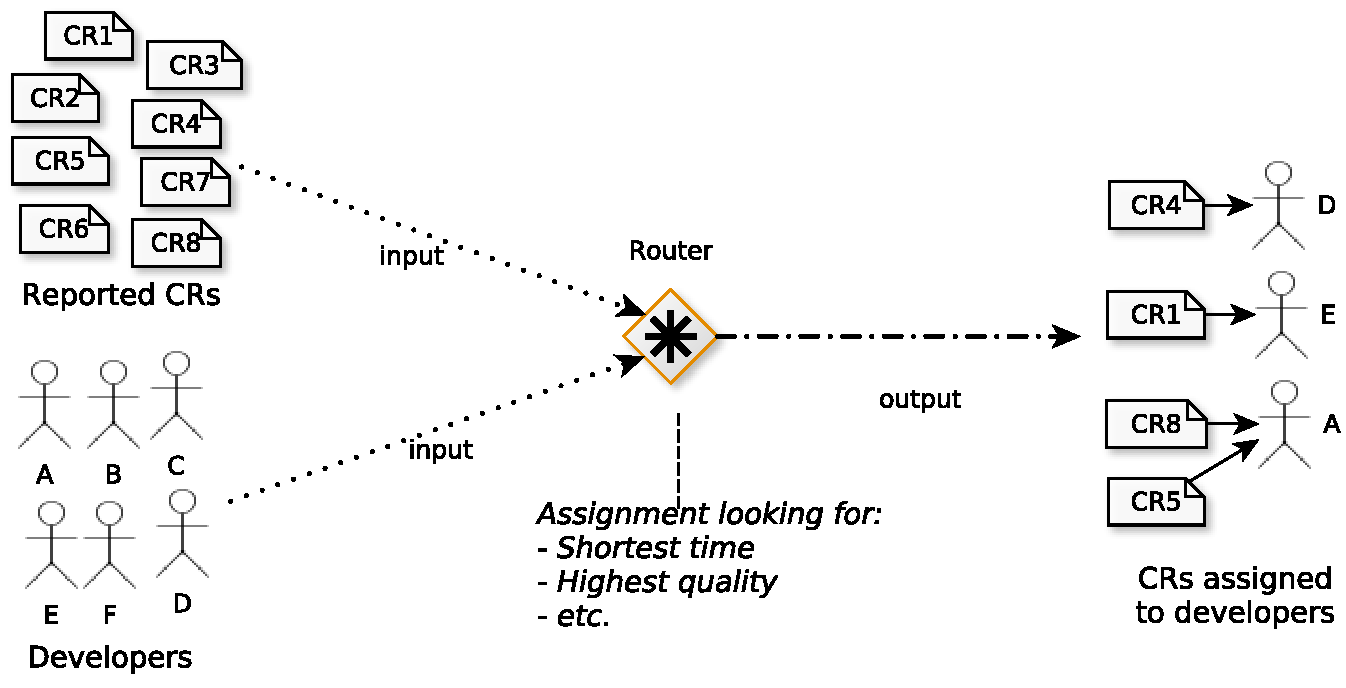
\includegraphics[width=\columnwidth]{images/assignment-schema.pdf}
%   \caption[\ac{cr} assignment.]{\ac{cr} assignment. The router, which may be the
%   \acs{ccb}, project leaders, or managers, must match \acp{cr} and developers in
%   order to obtain the shortest fixing and highest quality.}
%   \label{fig:assignment-schema}
% \end{figure}

% \lipsum[2-4]

% Nevertheless, by increasing the amount of reported \acp{cr} or the size of the
% development team, it is visible that the router becomes overloaded and the
% \ac{cr} assignment becomes an intensive, error prone activity. It was confirmed
% by \citet{Jeong2009}, which identified that 37\%-44\% of the \acp{cr} in Mozilla
% and Eclipse projects did not reach the right developer in the first assignment.
% These \acp{cr}, in turn, had their fixing time delayed because they needed to be
% reassigned one or more times. Furthermore, if the \acp{cr} are not fixed by the
% appropriate developers, there is also the chance of introducing new defects
% during the \acp{cr} fixing.

% In this context, we believe that it is necessary to develop methods and tools to
% automate the assignment of \acp{cr} and ensure that the \acp{cr} are being
% assigned to the appropriate developers. With these methods and tools, we could
% reduce the time needed to perform the assignments and, given that the
% appropriate developers are actually being selected, the quality and time for the
% \ac{cr} fixing are also improved.

\section{Objetivo}
\label{sec:objetivo}

 — Apresentar e discorrer sobre o objetivo do projeto em si. — 

% As previously mentioned, software maintenance has been considered as the most
% costly aspect of software development~\citep{swebok2004}. There is a myriad of
% reasons for this situation. One of them is the many changes that are required
% after software delivery due to poor documented and misunderstood requirements,
% or simply because \emph{``the clients do not know what they
% want''}~\citep{Brooks1995}.

% Another reason is the fact that a set of development activities must be
% inevitably performed in order to implement a change. For instance, for each
% change to be implemented it is necessary to comprehend the existing software
% artifacts, modify the software's source code to implement the change, perform
% tests and verification, and deliver the new version of the software.
% Additionally, very often, the implementation of the change ends up by
% introducing new defects in the software.
   
% A third reason is the management aspects of software maintenance. It is
% necessary to keep track of all these changes that are performed, generally
% considering different versions of the software and customers.

% \lipsum[3-5]

% \begin{enumerate}
%   \item Firstly, the approaches available in the literature were designed to
%   perform autonomously. That is, the software analysts do not have the control
%   of the approach; they cannot modify the approach's behavior. Without
%   such control, in turn, the approach cannot be properly calibrated. As a
%   consequence, if the approach's performance is not satisfactory, it is simply
%   discarded.
%   \item Secondly, the reported values for accuracy of these approaches are
%   still low. With low accuracy, the previous reason takes place. That is, as the
%   approaches perform with low accuracy, and the software analysts do not have
%   control over them, the approaches are simply discarded.
%   \item Finally, the third reason concerns the lack of contextual information in
%   those approaches. As is well known, software development companies are
%   dynamic: developers move from projects; developers are hired/fired;
%   developers enter in vacation or take a day off; and developers have different
%   experiences. This dynamic influences the assignment of \acp{cr}. Thus,
%   contextual information is a necessity in automated approaches.
% \end{enumerate}

% Based on this context, the main research question investigated by this thesis is:

% \begin{description}
%   \item[Research question] \emph{Is it possible to develop a new approach for
%   automated \ac{cr} assignment with satisfactory accuracy, leveraging
%   contextual information, and designed in order to put the software analysts in
%   control of such approach?}
% \end{description}

% With the objective to answer this question, it is necessary to understand
% current approaches available in the literature, choose the correct technologies
% that could support dynamic environments and, mainly, understand the necessities
% of software analysts regarding a new approach for automated \ac{cr} assignment.
% Thus, the goal of the work described in this thesis can be stated as:

% \begin{description}
%   \item[Research objective] \emph{This work proposes an automated approach for
%   \ac{cr} assignment which uses \ac{ir} models, expert systems, and
%   context-aware information in order to select the appropriate developers. The
%   approach is supported by the state-of-the-art in the management of \acp{cr} as
%   well as by the understanding of the aspects concerning the \ac{cr} assignment
%   activity itself.}
% \end{description} 

\section{Visão geral da proposta}

 — Apresentar e discorrer sobre o objetivo do projeto em si. — 

% \section{Research Methodology}

% This research design of this thesis is based on a multimethod
% approach~\citep{Hesse-Biber2010}. Such approach combines two or more
% quantitative (or qualitative) methods in a single study, such as a survey and an
% experiment~\citep{Hesse-Biber2010}. Multimethod must not be confused with mixed
% method. In this last, methods for both qualitative and quantitative types of
% research are applied in a single study. On the other hand, multimethod studies
% combine different methods for a single research type.

% When applying a multimethod approach, the triangulation is used to consolidate
% the results from the different methods, considering, however, that the same
% research question(s) was/were investigated in these methods. As a consequence,
% the triangulation of methods enhances the conclusions and completeness of the
% study, bringing more credibility to the research
% findings~\citep{Hesse-Biber2010}. \figref{fig:research-methodology-thesis} shows
% the multimethod research design applied in this thesis.

% \begin{figure}[h]
% \centering
%   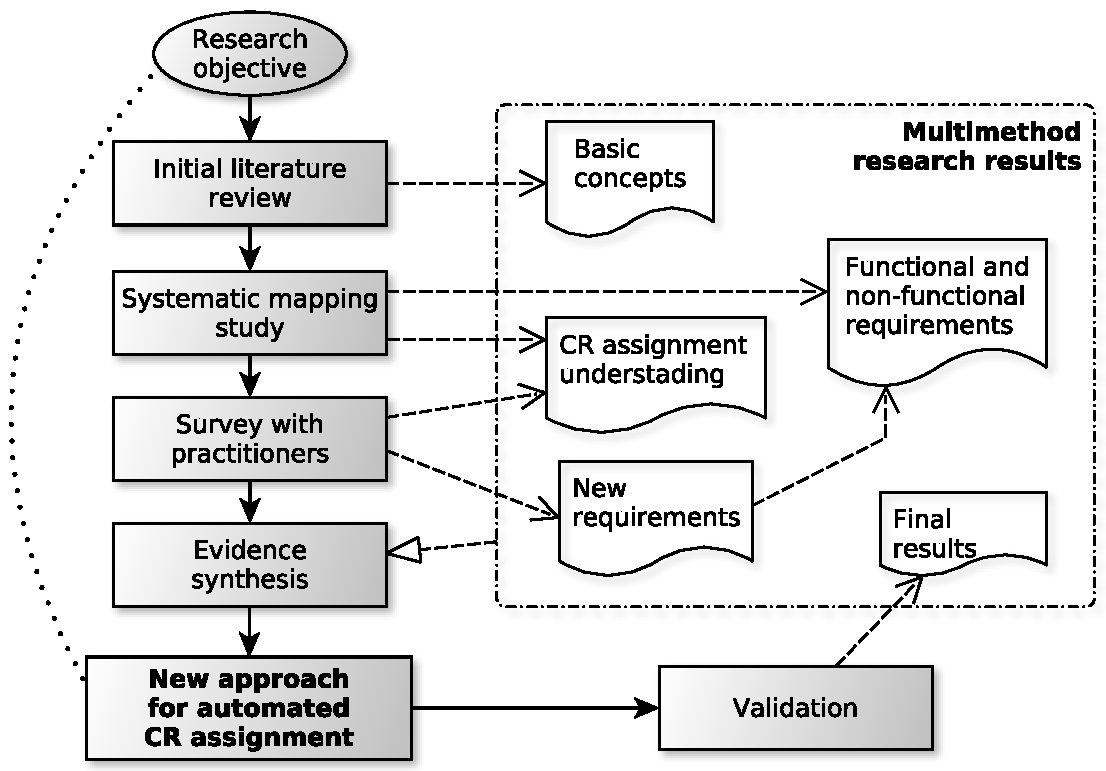
\includegraphics[width=\columnwidth]{images/research-methodology-thesis.pdf}
%   \caption[Research methodology.]{The research methodology applied for this
%   thesis.}
%   \label{fig:research-methodology-thesis}
% \end{figure}

% The design started by stating the research objective, which we defined in
% \secref{sec:intro-problem-statement}, and performing the initial literature
% review. This last provided the basic concepts and understanding of the area.
% Then, a systematic mapping study and a questionnaire-based survey were
% conducted. These two gathered detailed information on our research topic.
% Indeed, both of them were used to understand the key aspects of \ac{cr}
% assignment and identify the set of requirements to automate the assignments. In
% the evidence synthesis step, these results were detailed and organized in order
% to formulate the approach to automate \ac{cr} assignments, which was constructed
% in the next step. Finally, the research design states the validation of the
% proposed approach.

% \section{Out of Scope}

% As the proposed approach is part of a broader context, a set of related aspects
% will be left out of its scope. Thus, the following topics are not directly
% addressed in this thesis:

% \begin{enumerate}
%   \item \textbf{Tools for \ac{cr} management.} We are addressing
%   a specific aspect of \ac{cr} management, which is the \ac{cr} assignment
%   activity. Thus, it is out of scope of this thesis to provide a
%   complete solution for \ac{cr} management. Instead, we are planning to
%   implement standalone software which will be able to integrate with the
%   most well known tools for \ac{cr} management, such as Mantis, Bugzilla, and
%   Trac, providing a service to leverage the automation of \ac{cr}
%   assignments.
  
%   \item \textbf{Software maintenance process.} Software maintenance involves
%   a set of activities aiming at implementing modifications in some software
%   project. These activities must be coordinated through a process so that the
%   maintenance can be successful. In Chapter 2, we discuss some of
%   these processes. However, in this thesis, we are not concerned with the
%   maintenance process itself. Actually, it should be transparent in our approach
%   to automate \ac{cr} assignment. Thus, it is out of scope of this
%   thesis to provide any process assessment for software maintenance beyond the
%   activity of \ac{cr} assignment.
  
%   \item \textbf{\ac{ir} models.} Many models for \ac{ir} have been proposed for
%   different objectives, including the \ac{cr} assignment itself. However, due to
%   the broad availability of these models, it is out of scope of this thesis to
%   develop a new one. Instead, the \ac{ir} models with better performance,
%   identified through the systematic mapping study, were chose to be
%   integrated in our approach;
  
%   \item \textbf{Rule-based expert systems.} Similar to \ac{ir} models,
%   rule-based expert systems have a long history of development. Thus, our
%   approach does not intend to develop a whole new system with this purpose.
%   Actually, we integrated in our approach the
%   Drools\footnote{\url{http://www.jboss.org/drools/}} expert system, which is a
%   mature tool that can be easily manipulated;
  
%   \item \textbf{Mathematical formulations on NP-Complete problems.} We
%   understand that the problem of assigning \acp{cr} to software developers is in
%   the broad category of \emph{assignment problems}, which is well known to be
%   NP-Complete. Thus, could be formulated as such. However, the mathematical
%   formulations of the \ac{cr} assignment problem is out of scope of this thesis.
%   As well as finding an optimal solution on the context of NP-Complete problems
%   is also out of scope. The main reason for this is the human factors and
%   context variables that are involved in the assignment of \acp{cr}, which
%   make this problem hard to be computable. A mathematical formulation of the
%   \ac{cr} assignment problem is provided by~\citet{Rahman2009}.
% \end{enumerate}

% \section{Statement of the Contributions}
% \lipsum[6-7]

% \begin{enumerate}
%   \item An overview of the software maintenance concepts and processes, with
%   emphasis on the importance of \ac{cr} management aspects; 
%   \item A survey performed with practitioners from a large organization, in
%   order to understand the aspects of the \ac{cr} assignment
%   activity. Published in the \emph{17$^{th}$ International Conference on Evaluation
%   and Assessment in Software Engineering (EASE'2013)}~\citep{CavalcantiEASE2013};
%   \item A replication of the previous survey in two more organizations;
%   \item A systematic mapping study performed to understand the challenges and
%   opportunities of \ac{cr} management, as well as to identify research gaps and
%   the road ahead. Accepted for publication in the
%   \emph{Journal of Software: Evolution and Process}~\citep{CavalcantiJSEP2013};
%   \item The definition of the functional and non-functional requirements that
%   are required to effectively automate \ac{cr} assignment, which takes as input
%   the systematic mapping study and the survey;
%   \item The definition of an approach that satisfies the
%   identified requirements to automate the \ac{cr} assignment activity;
%   \item The realization of the proposed approach's architecture, in which we
%   described the methods and techniques used for the implementation, as well as the
%   components that have to be built and the third party components that should be
%   assembled together in order to provide a service for automated \ac{cr}
%   assignment; and
%   \item The evaluation of the proposed approach, performed as an offline
%   experiment simulating a real context.
% \end{enumerate}

\section{Organização do texto}

 — Apresentar e discorrer sobre a 
 organização do texto do projeto. — 

% \lipsum[5-10]
\chapter{Fundamentação Teórica}

\section{Mobilidade}\label{sec:mobilidade}
Segundo \citet{b2004mobile}, um sistema de computação móvel é um sistema que pode ser facilmente movido fisicamente ou cuja funcionalidade pode ser usada durante o movimento. Como esses sistemas fornecem essa mobilidade, essas funcionalidades adicionadas são a razão para caracterizar separadamente os sistemas de computação móvel, eles geralmente oferecem capacidades e recursos não encontrados em sistemas normais, como: 
 \begin{itemize}
   \item Armazenamento de dados local e/ou remoto via conexões com ou sem fio;
   \item Segurança para persistência de dados em caso de queda de energia ou pane;
   \item Sincronização de dados com outros sistemas;
   \item Etc.
 \end{itemize}

Atualmente, pensamos em um sistema móvel como um sistema projetado para rodar em um computador de mão, seja ele celular, tablet ou qualquer outro dispositivo com tais características. Pela definição acima, os notebooks também são considerados plataformas para sistemas móveis, mas não são utilizados exatamente da mesma forma que os dispositivos citados acima, pois precisa parar em algum lugar, abrir o notebook, esperar carregar, etc...

\section{Dispositivos móveis}\label{sec:dm}
Para adentrar no universo da solução apresentada, \ac{dm}, é valioso abordar como estes \textit{gadgets} lidam com a capacidade de armazenamento e processamento de dados, que, por possuírem sistemas móveis espera-se que os mesmos possuam menor eficiência para desenvolver atividades se comparados a um computador estacionário (\ac{pc}), por exemplo, que possui muito mais disponibilidade energética para realizar suas tarefas, porém, nos dias de hoje esse \textit{gap} para atividades cotidianas está mais estreito, devido aos grandes avanços da tecnologia voltados a este segmento que vem em forte alta (o qual, segundo \citet{data.ai} cresceu 20\% em 2020 comparado ao ano anterior, gerando um consumo no valor de 143 bilhões de dólares no mundo todo, mesmo com as dificuldades enfrentadas pela pandemia da COVID-19, vale ressaltar que há uma expectativa que o mercado de \acp{dm} cresça ainda mais até 2026 \cite{mordor_intelligence_2021}), já para processamentos mais robustos estamos caminhando em largos passos, atualmente é possível se deparar com sistemas móveis utilizando o processamento em nuvem (que são outra forma de representação de sistema estacionários, um exemplo disso são os servidores computacionais) para tais atividades, enquanto outros \acp{dm} já contam com \textit{chipsets} dedicados exclusivamente para isso.

Para situar onde os \acp{dm} chegaram, é preciso olhar um pouco o passado para lembrar como os computadores eram: máquinas que ocupavam salas gigantes, os quais eram manuseados somente por setores importantes da sociedade, antes mesmo de ser um dispositivo doméstico como é hoje, limitando-se a órgãos do governo, instituições de ensino e poucas empresas, por exemplo. \citet{alecrim_2013}.

Com o desenvolvimento da tecnologia, os computadores tornaram-se cada vez mais compactos, eficientes, práticos e fáceis de usar, podendo ser levados para qualquer lugar, por qualquer pessoa. As tecnologias que fornecem essa maior flexibilidade são conhecidas como \acp{dm}.

Sintetizando, um \ac{dm} é um tipo de dispositivo computacional que tem como principais características a portabilidade, a compactabilidade e fácil manuseio \citet{lee2005aplicaccoes}, além de todos os aspectos citados na seção \ref{sec:mobilidade}. 

De acordo com \citet{laricchia_2022}, em 2021, o número de \acp{dm} operando em todo o mundo ficou em quase 15 bilhões, contra pouco mais de 14 bilhões no ano anterior. Espera-se que o número de \acp{dm} atinja 18,22 bilhões até 2025, um aumento de 4,2 bilhões de dispositivos (aproximadamente 30\%) em comparação com os níveis de 2020. A \figref{fig:mobiles20to25} mostra o gráfico desta previsão.

\begin{figure}[h]
\centering
  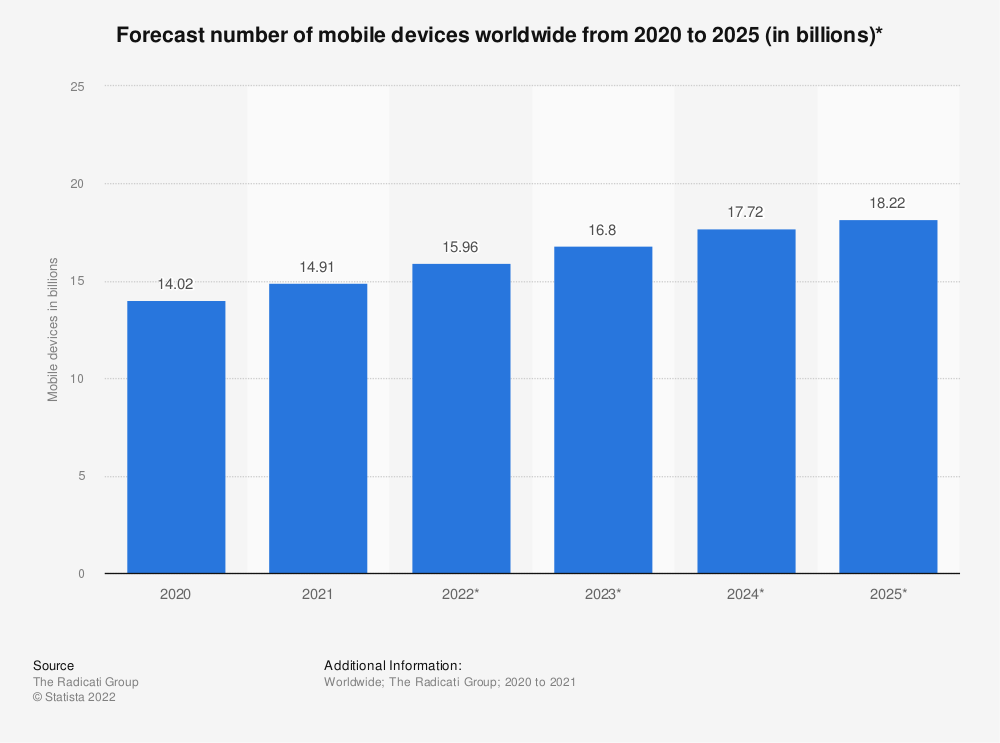
\includegraphics[width=\columnwidth]{images/mobiles20to25.png}
  \caption{Previsão do número de dispositivos móveis em todo o mundo de 2020 a 2025 (em bilhões)}
  \label{fig:mobiles20to25}
\end{figure}

Visto esse crescimento no uso de \acp{dm}, é perceptível que a demanda por \textbf{desenvolvimento de \textit{software}} para esta tecnologia também está aumentando. Essas soluções são chamadas de aplicativos móveis, o qual será abordado com mais detalhes na seção \ref{sec:apps} e posteriormente detalhado sobre o mercado de desenvolvimento de aplicativos na subseção \ref{ssec:dev_apps}.

\subsection{iOS}\label{ssec:ios}
\lipsum[1]


\subsection{Android}\label{ssec:android}
\lipsum[1]


\section{Aplicativos móveis}\label{sec:apps}
\lipsum[1]


\subsection{Desenvolvimento de aplicativos}\label{ssec:dev_apps}
\lipsum[1]

\subsubsection{Desenvolvimento nativo}\label{sssec:dev_apps_nativo}
\lipsum[1]

\subsubsection{Desenvolvimento híbrido}\label{sssec:dev_apps_hibrido}
\lipsum[1]


\section{[ abordar sobre o tema do app, area que es'ta associada à agronomia, etc... ]}
\lipsum[1]


\chapter{Metodologia}
Neste capítulo é apresentada a metodologia utilizada para o desenvolvimento do aplicativo. 
[EM DESENVOLVIMENTO até 31/03/23]

% Após o levantamento dos conceitos necessários para o desenvolvimento da aplicação e um estudo de aplicativos similares na literatura, o próximo passo foi um levantamento dos sistemas existente na CBMPA. Revisão bibliográfica: descrever as principais referências utilizadas para a construção da aplicação móvel, incluindo frameworks, bibliotecas e outras tecnologias relacionadas.

% Revisão bibliográfica: descrever as principais referências utilizadas para a construção da aplicação móvel, incluindo frameworks, bibliotecas e outras tecnologias relacionadas.

% Especificação de requisitos: descrever os requisitos funcionais e não funcionais da aplicação móvel, incluindo as funcionalidades que ela deve ter e as plataformas em que deve ser executada.

% Prototipagem: descrever o processo de prototipagem da aplicação móvel, incluindo a criação de wireframes, modelos de tela e fluxos de navegação.

% Desenvolvimento: descrever o processo de desenvolvimento da aplicação móvel, incluindo as ferramentas e tecnologias utilizadas, como a linguagem de programação, banco de dados e plataformas de desenvolvimento.

% Testes: descrever o processo de testes da aplicação móvel, incluindo os tipos de testes realizados, como testes funcionais e de desempenho.

% Implantação: descrever o processo de implantação da aplicação móvel, incluindo a distribuição nas lojas de aplicativos, atualizações e manutenção.


\chapter{Desenvolvimento}

\section{Back-end}

\lipsum[1]

\section{Comunicação por API}

\lipsum[1]

\section{Aplicativo móvel desenvolvido}

% \subsection{Subsection}

\lipsum[1]
\chapter{Análise dos resultados}\label{ch:resultados}
A ideia deste capítulo é trazer uma visão geral sobre todas as funcionalidades desenvolvidas, o fluxo de navegação entre as \textit{features} e como o \ac{app} ficou em sua última versão.

\section{Apresentação do Enzitech}
Após concluído todos os requisitos funcionais, a versão final do Enzitech lida com dois tipos de usuário, Comum ou Administrador. O primeiro deles é referente ao perfil de todos os usuários, pessoas que utilizarão o sistema para criar e calcular seus experimentos. Já o segundo é destinado ao administrador geral de todo o sistema, normalmente uma única pessoa que ficará encarregada de gerir o Enzitech disponibilizando os dados corretamente. 

A diferença entre os dois perfis está na possibilidade de criação de enzimas, funcionalidade restrita ao Administrador, devido a necessidade de ajuste também no \textit{back-end}, ou seja, o Administrador fica responsável por gerir (criar e excluir) enzimas e solicitar a inclusão de novos cálculos para outros tipos, outro detalhe importante é que as enzimas criadas pelo Administrador ficam disponíveis para todos os usuários do sistema, as demais funcionalidades ficam disponíveis para ambos os tipos de usuário. 

Sendo assim, para ter acesso ao sistema, o usuário terá que inserir seus dados de acesso, e-mail e senha, na tela de login (\figref{fig:fluxo_login}). A autenticação é fundamental para que o usuário tenha acesso às funcionalidades do \ac{app}, o login satisfaz o caso de uso UC02.


\begin{figure}[H]
\centering
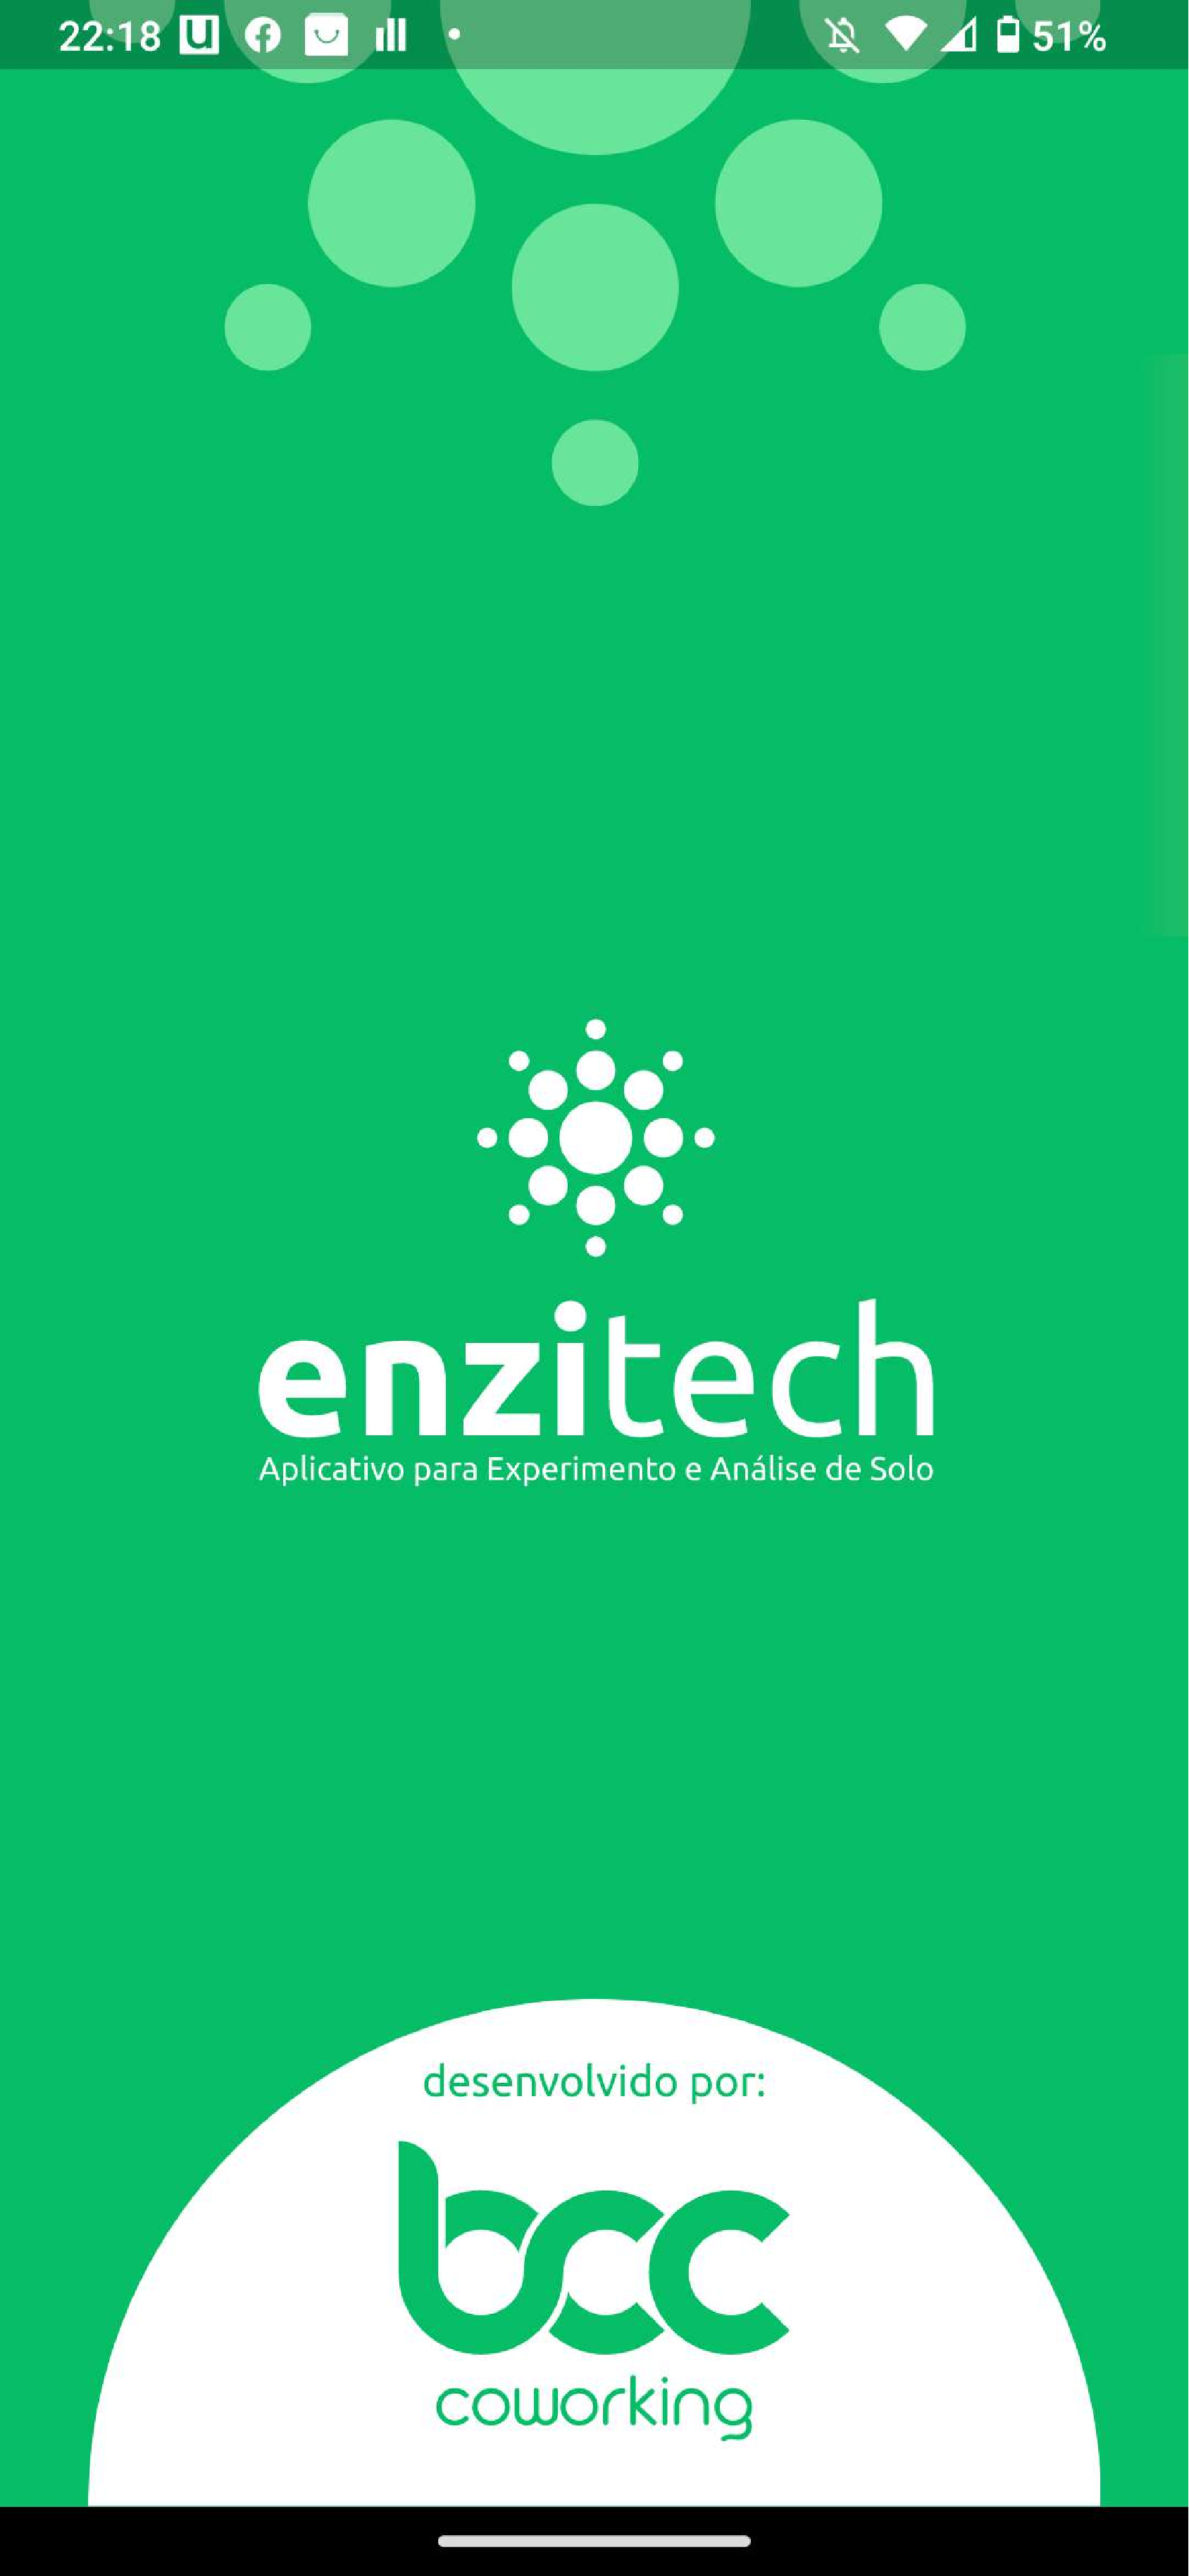
\includegraphics[width=.3\textwidth]{images/enzitech/splash.pdf}
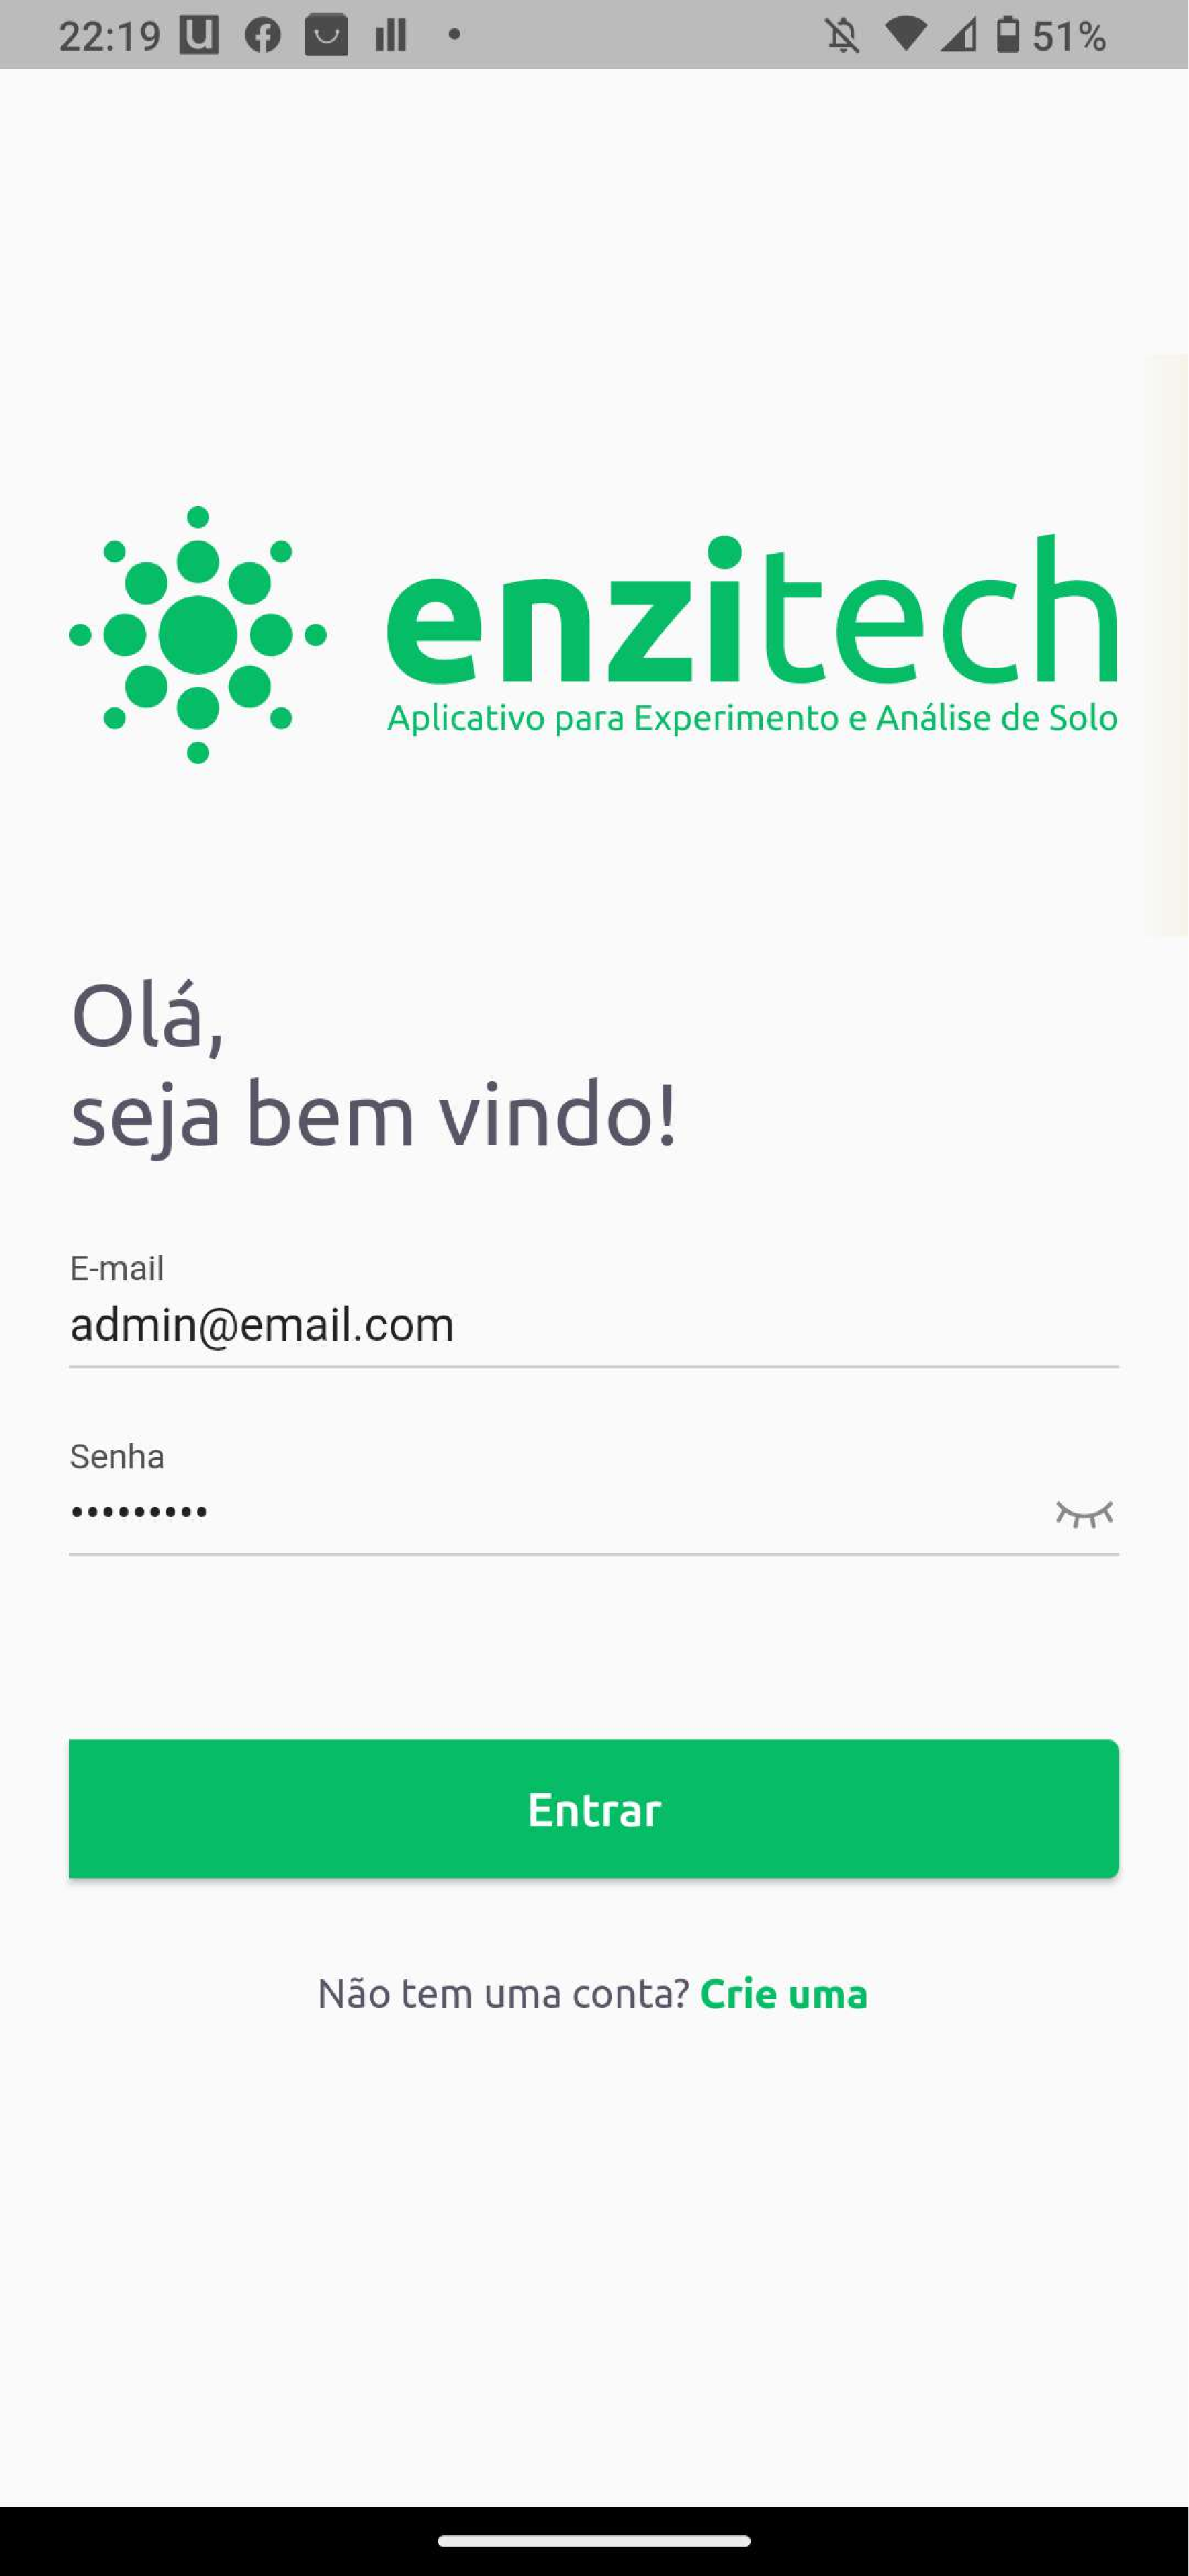
\includegraphics[width=.3\textwidth]{images/enzitech/login.pdf}
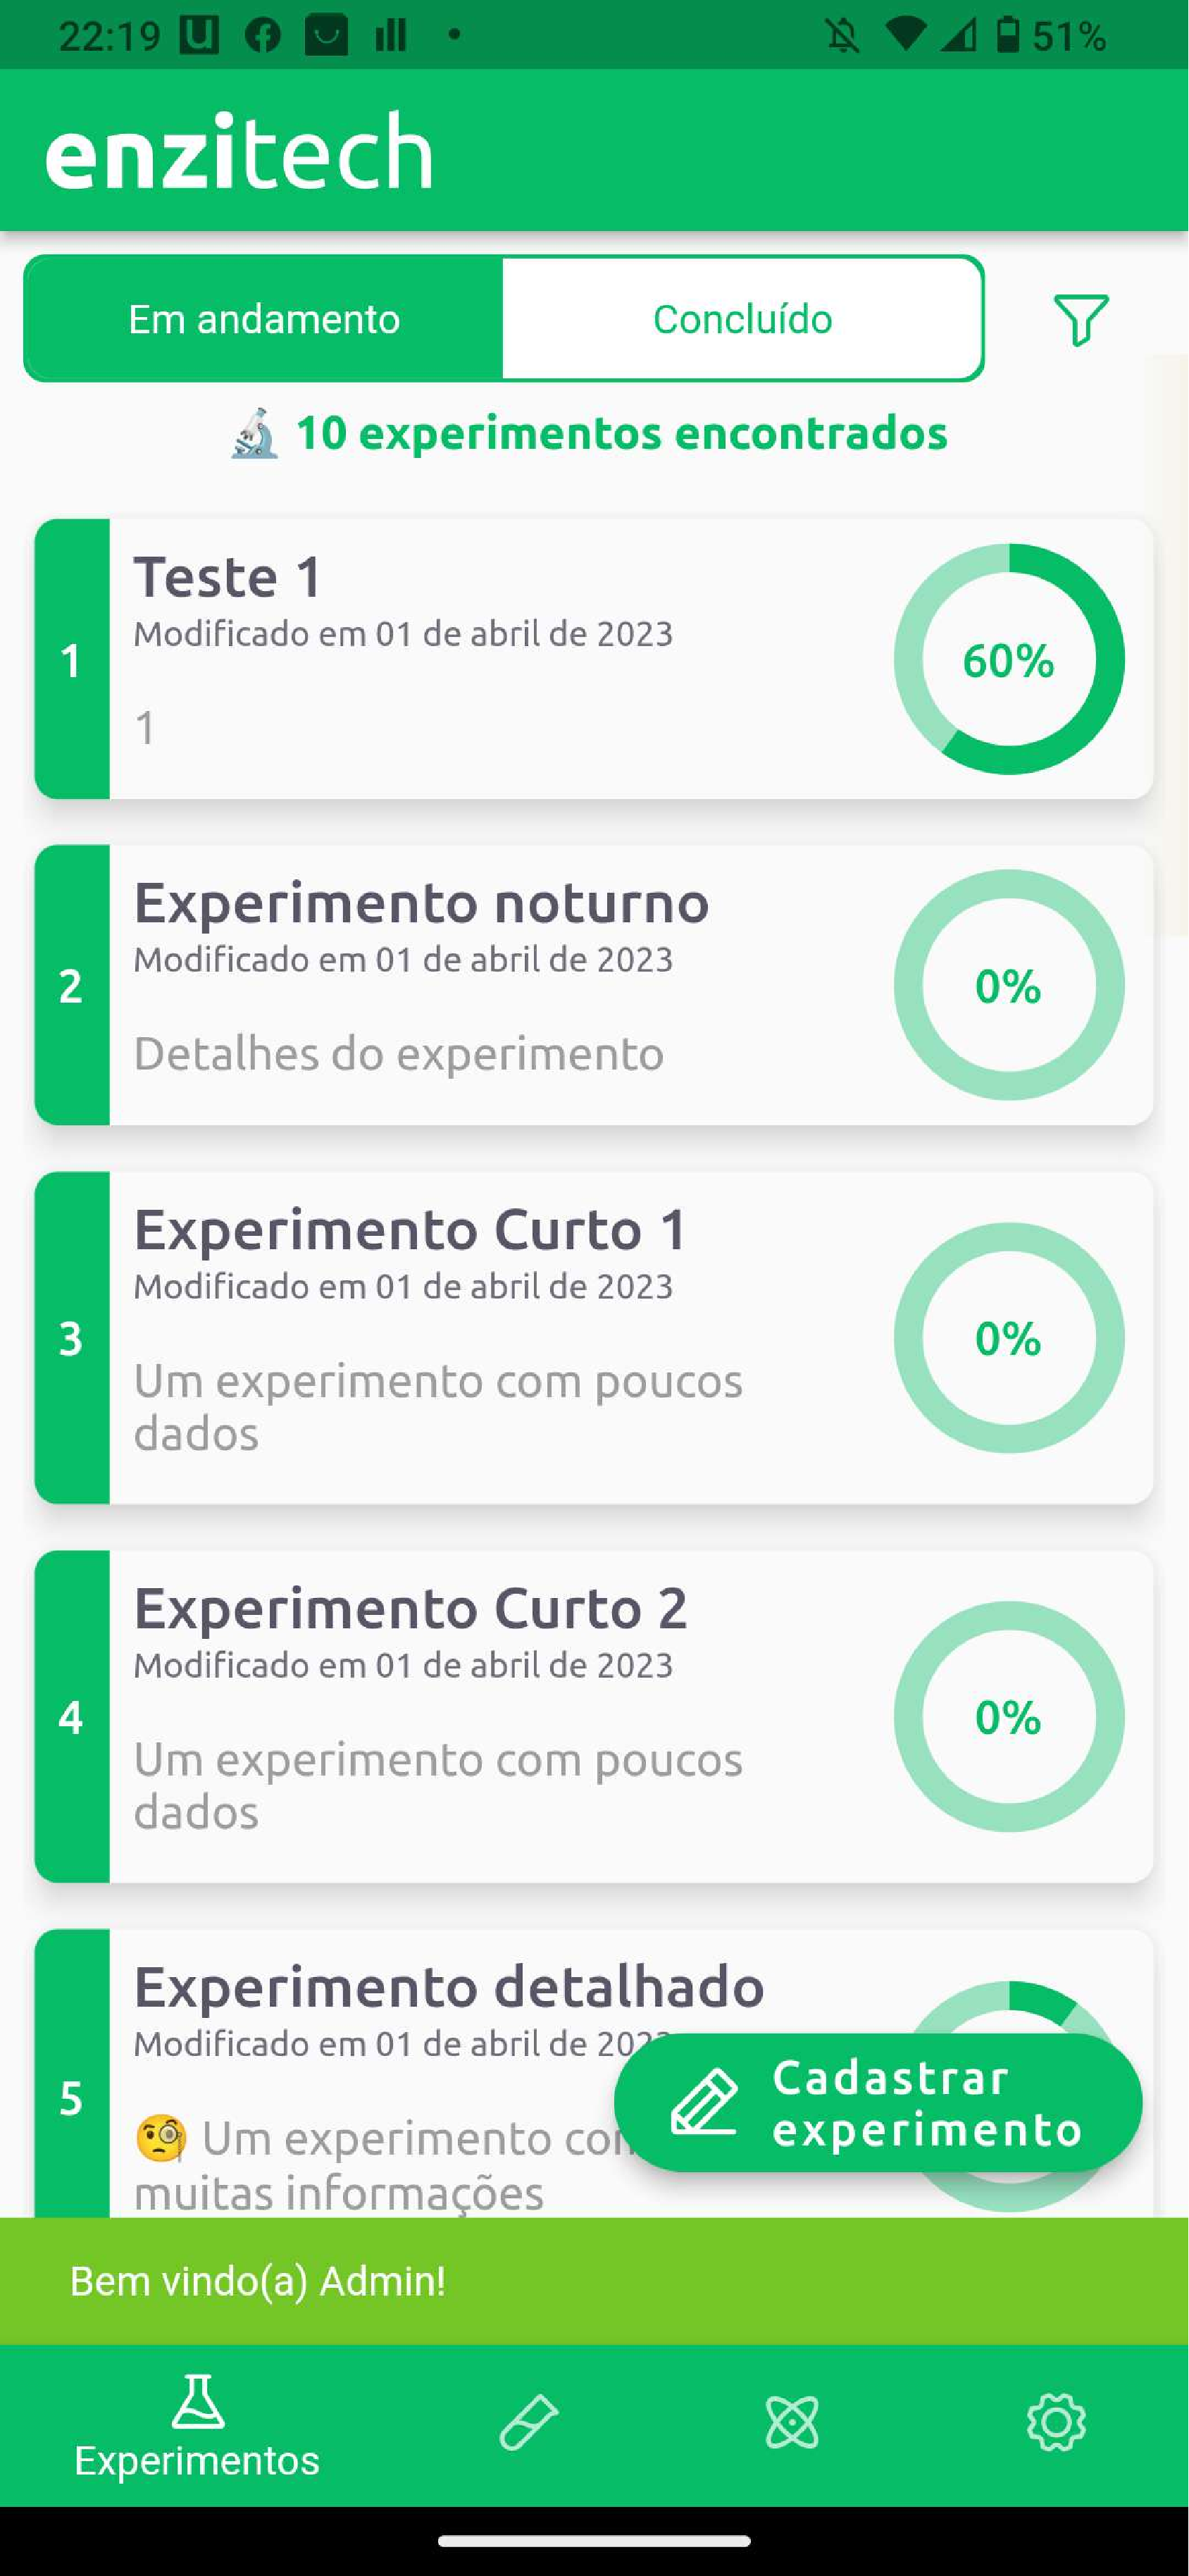
\includegraphics[width=.3\textwidth]{images/enzitech/home.pdf}
\caption{Fluxo de login do Administrador previamente cadastrado.}
\acsfont{Fonte: Aplicativo Enzitech desenvolvido pelo autor}
\label{fig:fluxo_login}
\end{figure}

Na \figref{fig:fluxo_login}, é possível ver o fluxo inicial do \ac{app}, ao abrí-lo, é feita uma verificação na \textit{splashscreen} (primeira imagem da sequência) para determinar se existe usuário logado ou não, caso negativo, o \ac{app} redireciona para a tela de login, onde é possível criar uma conta (caso de uso UC01), recuperar senha (caso de uso UC03) ou logar com suas credencias, após o login, ou, caso o usuário já estivesse logado, o app redireciona para a \textit{homepage}, onde estão todas as funcionalidades disponíveis, a primeira delas é a listagem de experimentos (caso de uso UC07), nesta tela é possível além da listagem, filtrar, excluir ou criar, como será mostrado em breve.

\begin{figure}[H]
\centering
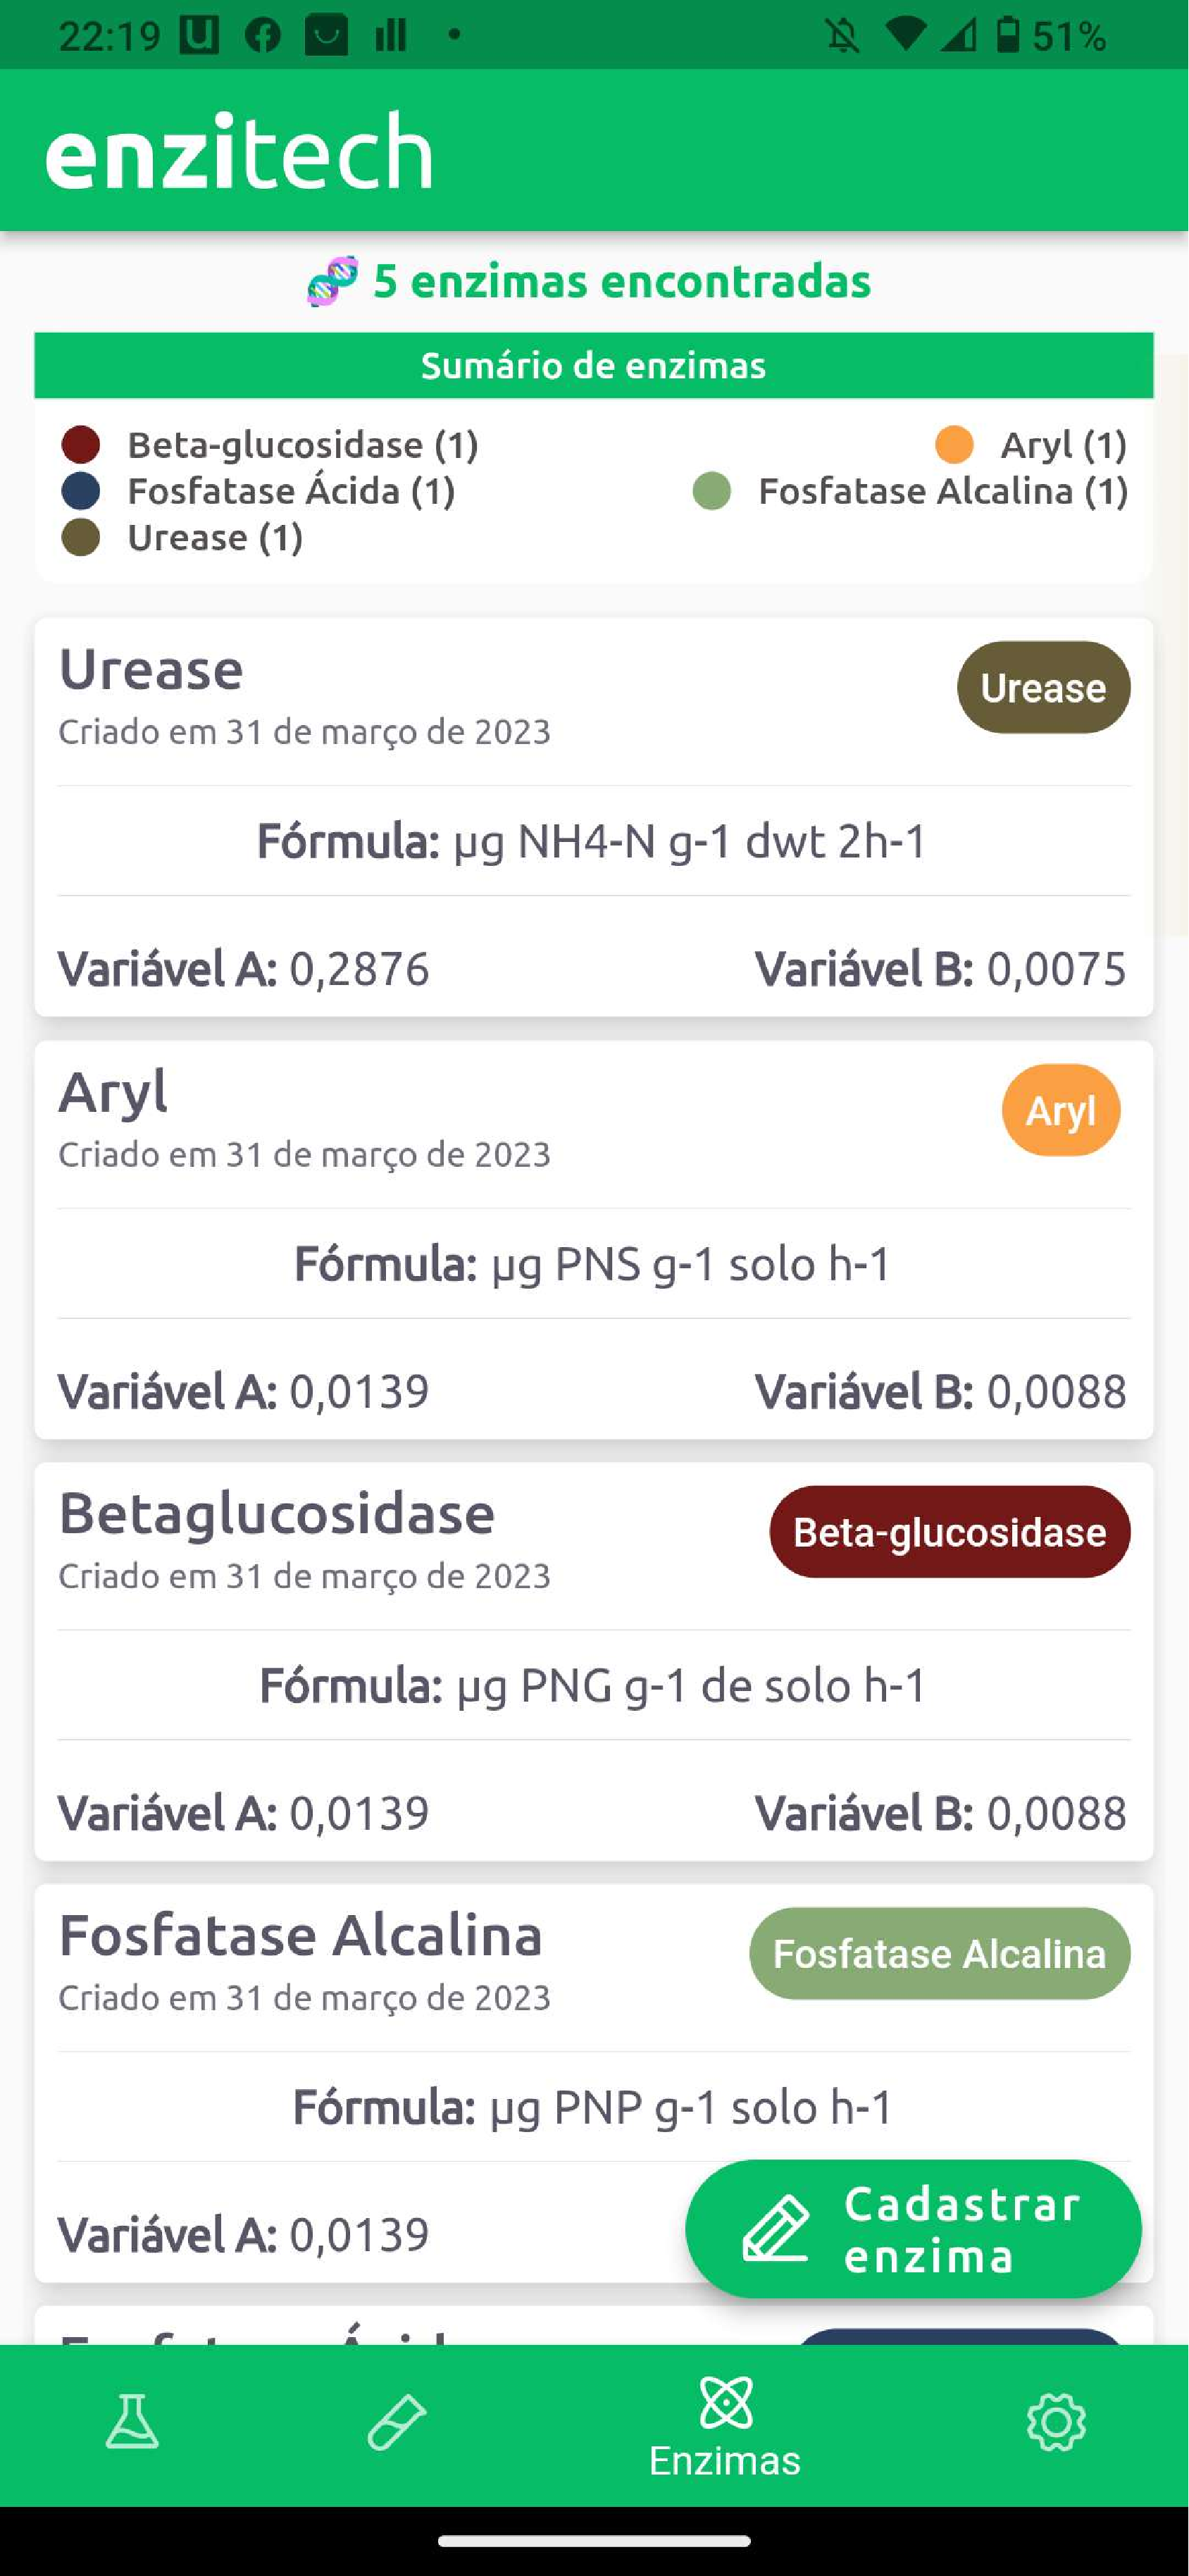
\includegraphics[width=.4\textwidth]{images/enzitech/enzimas.pdf}\hfill
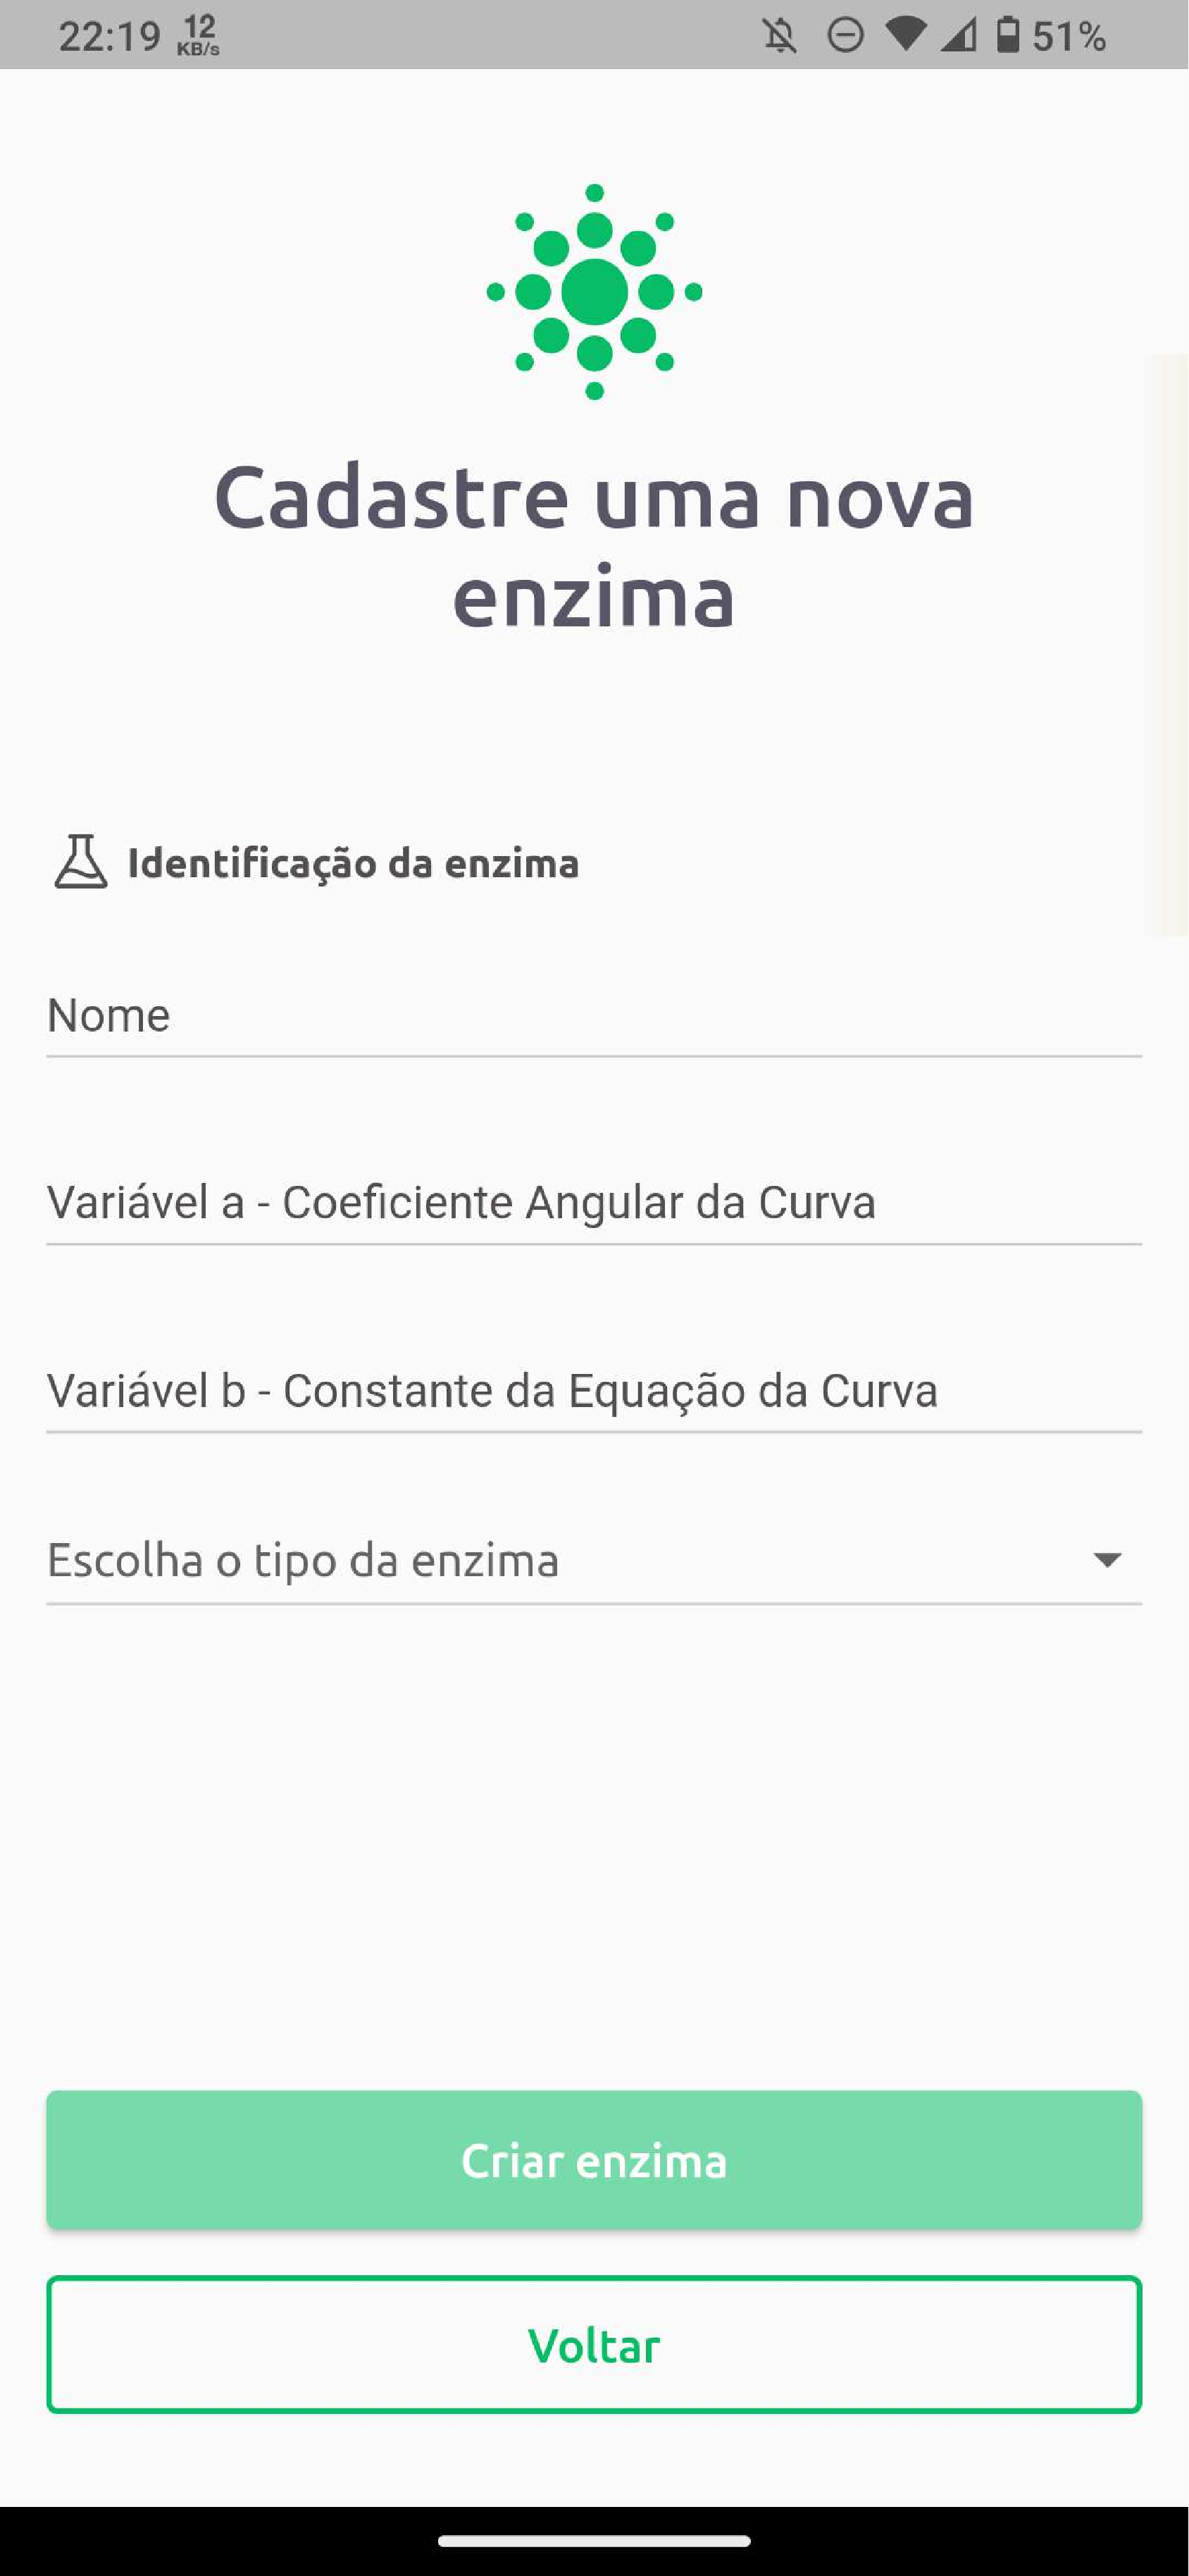
\includegraphics[width=.4\textwidth]{images/enzitech/cria_enzima.pdf}\hfill
\caption{Fluxo de listagem, exclusão e criação de enzimas.}
\acsfont{Fonte: Aplicativo Enzitech desenvolvido pelo autor}
\label{fig:fluxo_enzima}
\end{figure}

Na \figref{fig:fluxo_enzima}, estão as funcionalidades de listagem, exclusão e criação de enzimas, esta última restrita ao administrador, satisfazendo os casos de uso UC05 e UC06. Criar uma enzima no sistema é fundamental para a criação de um experimento.

Abaixo, na \figref{fig:fluxo_tratamento}, está o fluxo de listagem, criação e exclusão dos tratamentos (caso de uso UC04), a criação de um tratamento também é fundamental para a criação de um experimento.

\begin{figure}[H]
\centering
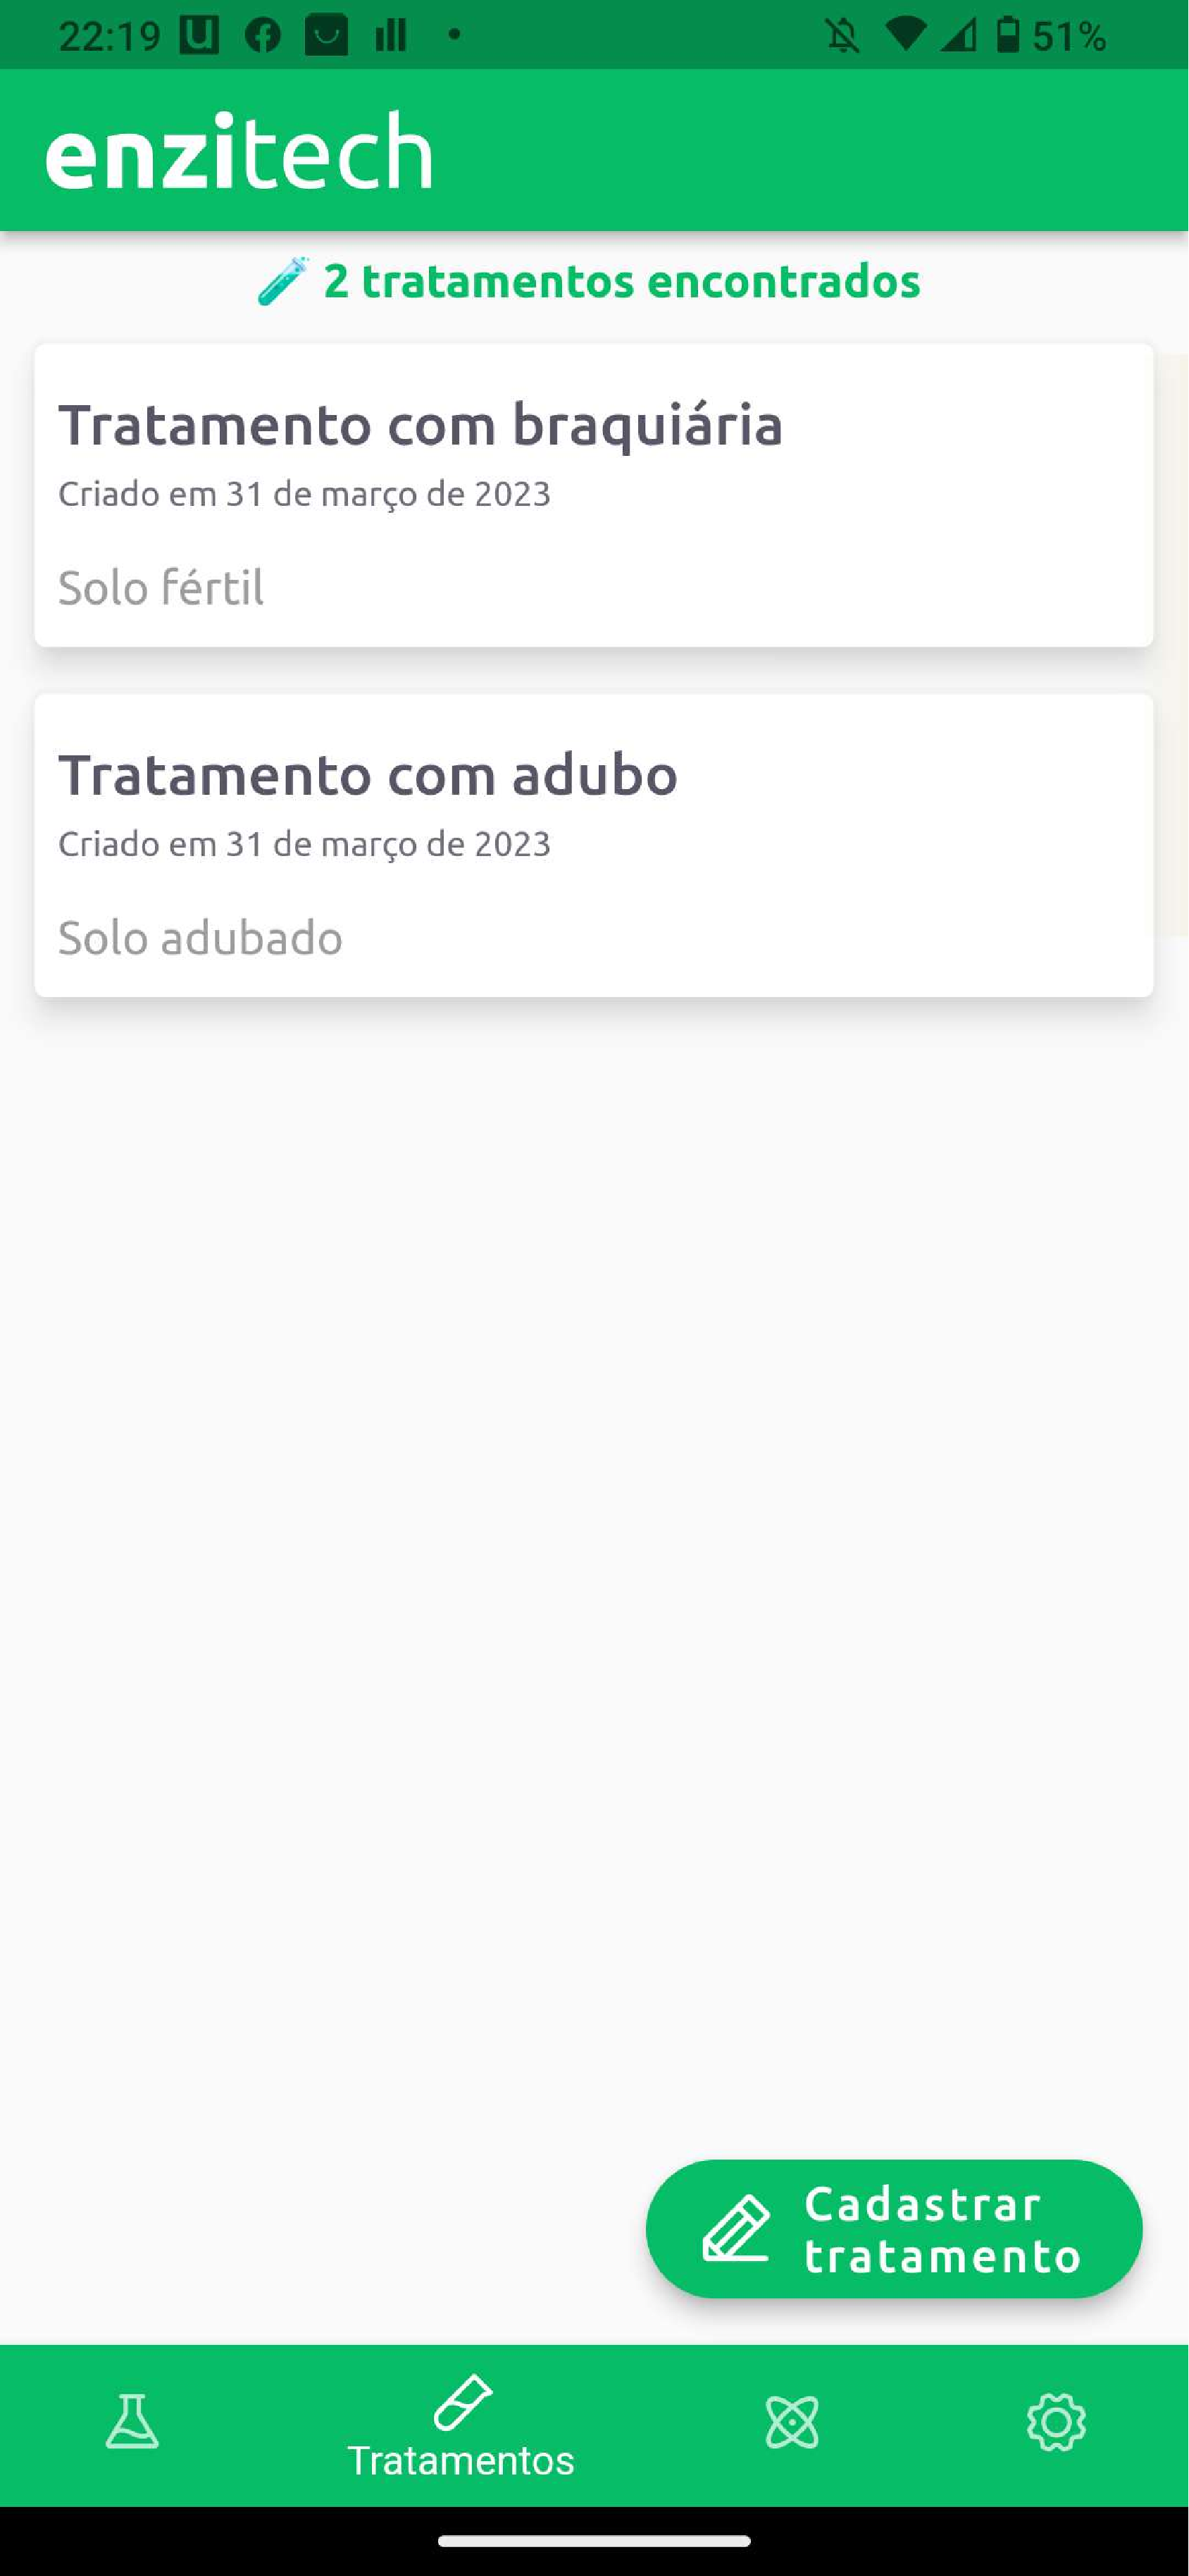
\includegraphics[width=.4\textwidth]{images/enzitech/tratamentos.pdf}\hfill
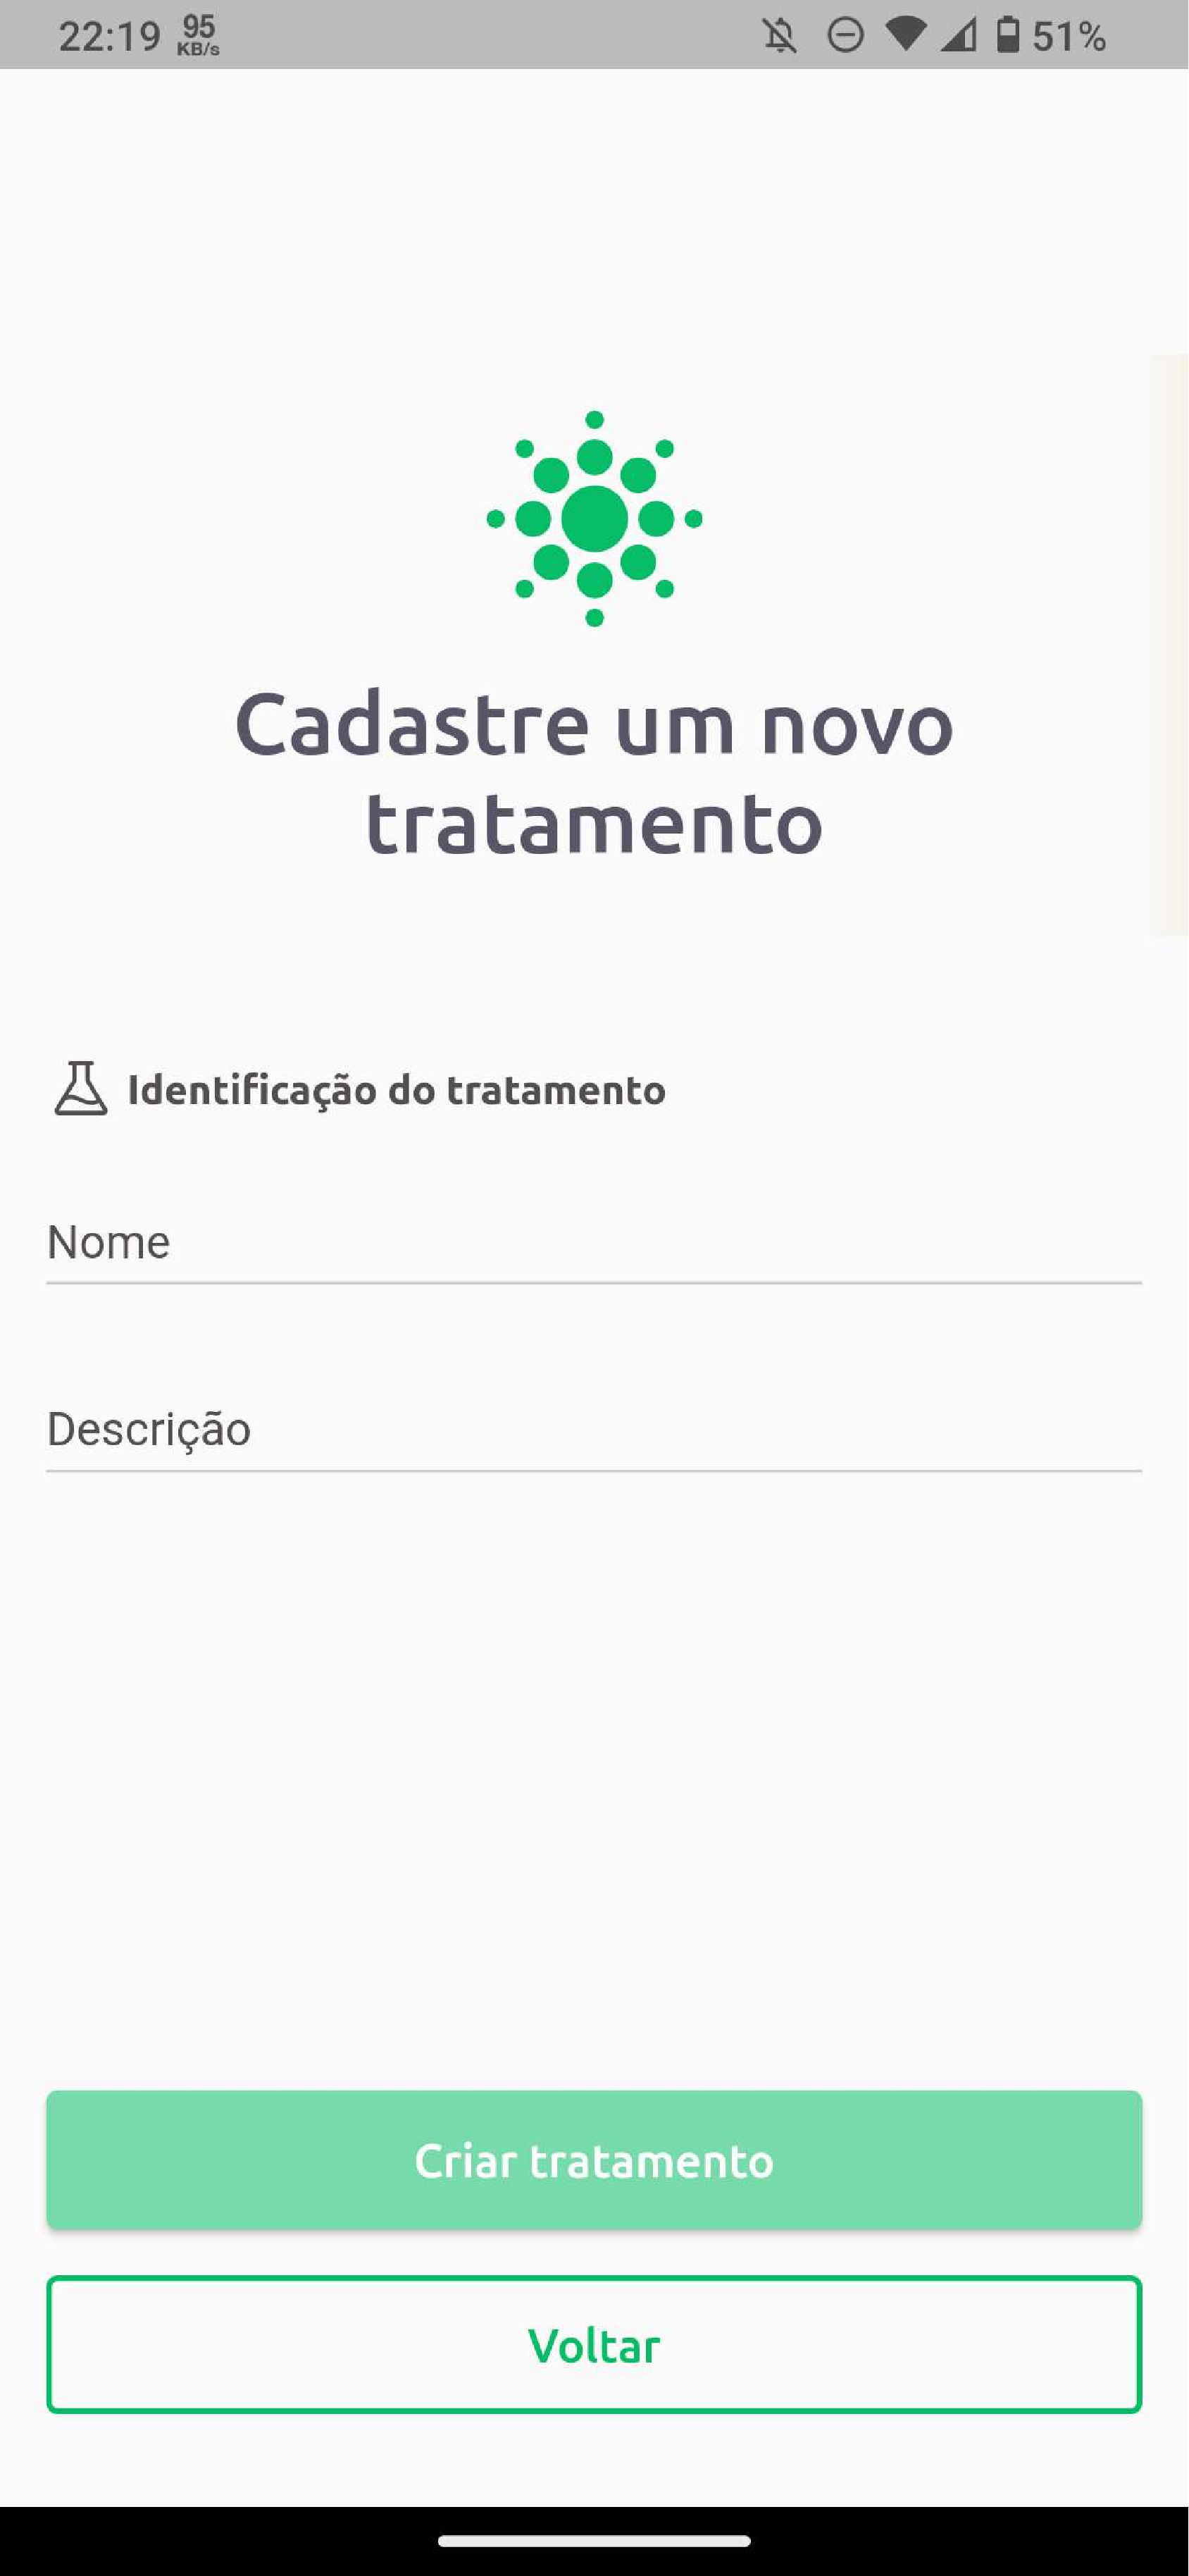
\includegraphics[width=.4\textwidth]{images/enzitech/cria_tratamento.pdf}\hfill
\caption{Fluxo de listagem, exclusão e criação de tratamentos.}
\acsfont{Fonte: Aplicativo Enzitech desenvolvido pelo autor}
\label{fig:fluxo_tratamento}
\end{figure}

Após criado pelo menos uma enzima e um tratamento, o usuário consegue criar seu primeiro experimento, como mostrado no fluxo da \figref{fig:fluxo_cria_experimento} abaixo.

\begin{figure}[p]
  \centering
  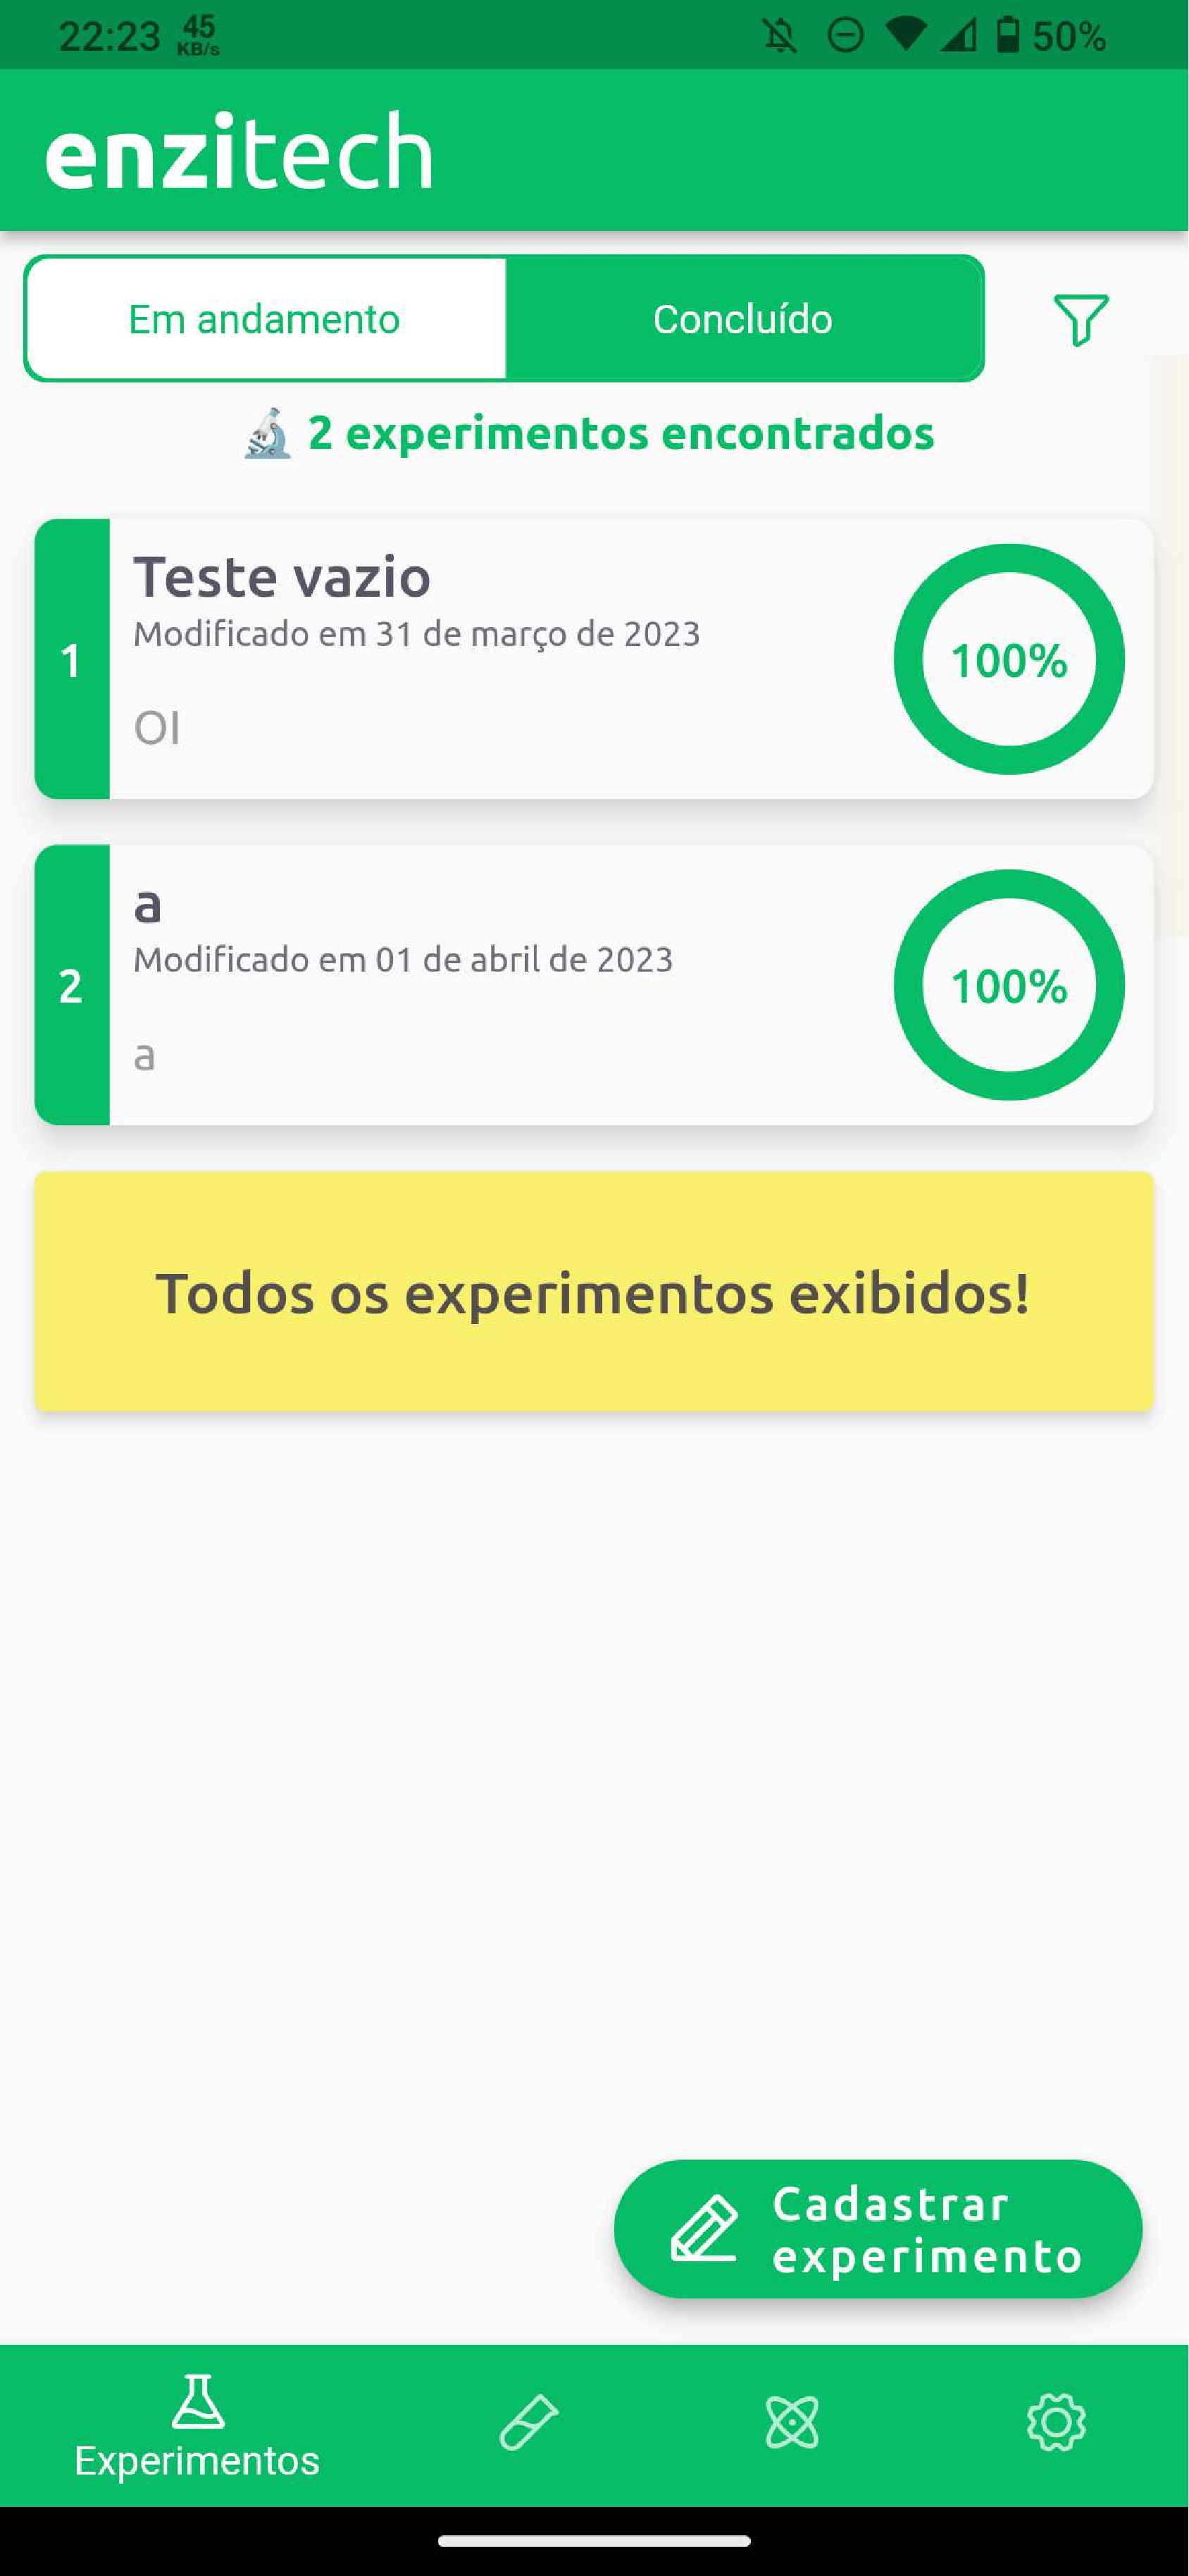
\includegraphics[width=.3\textwidth]{images/enzitech/home_2.pdf}
  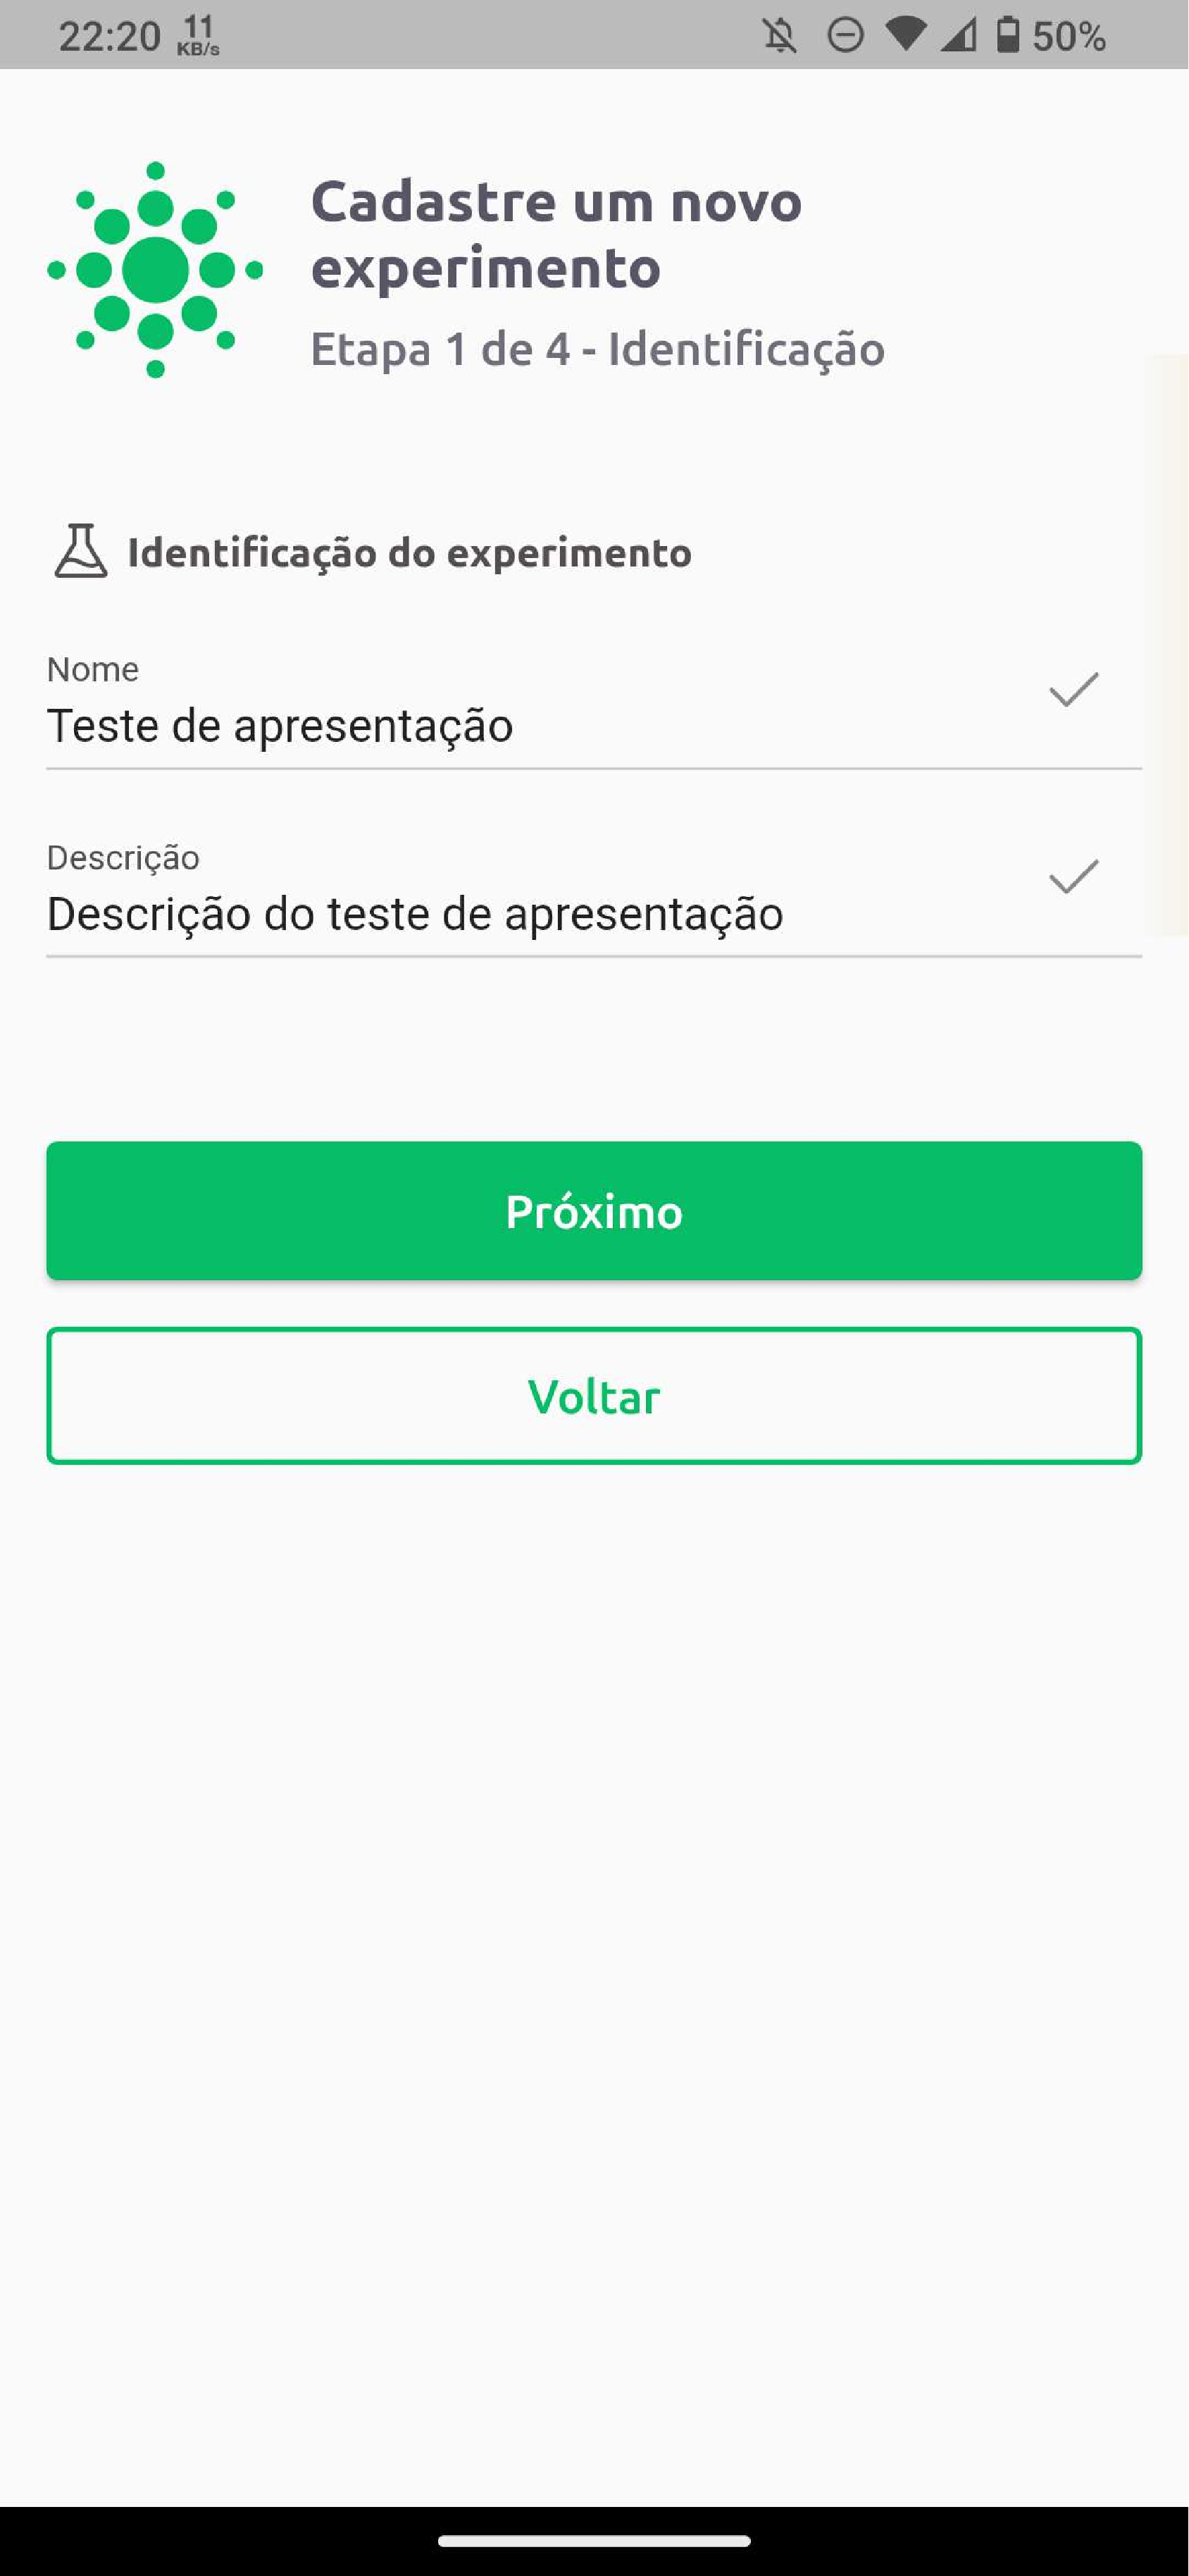
\includegraphics[width=.3\textwidth]{images/enzitech/cria_exp_1.pdf}
  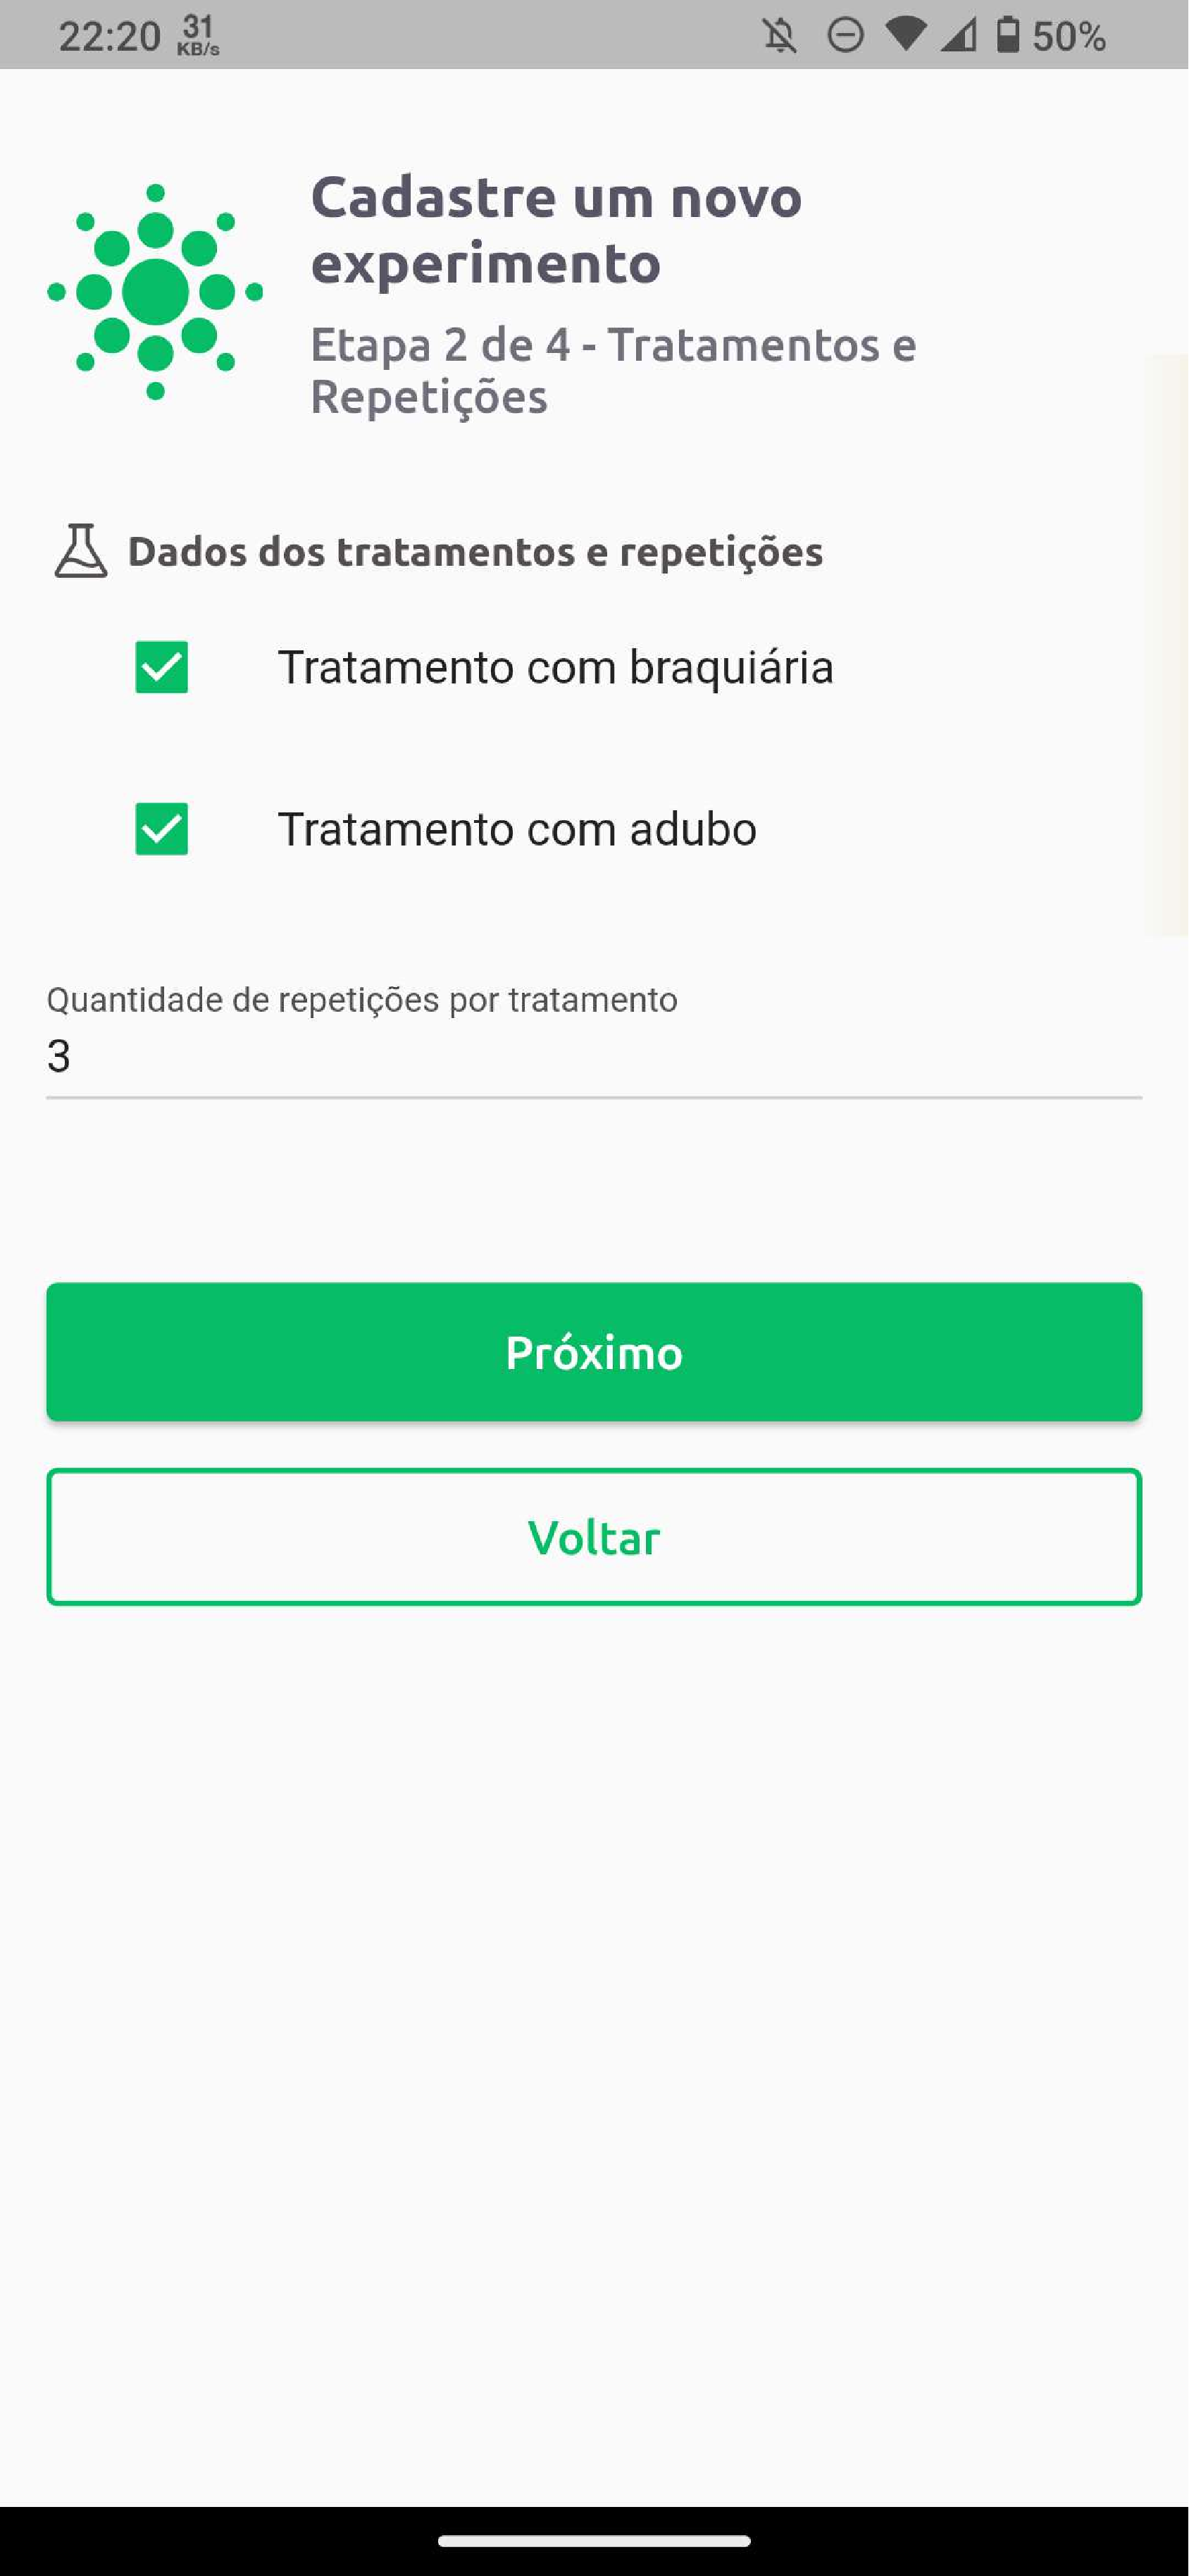
\includegraphics[width=.3\textwidth]{images/enzitech/cria_exp_2.pdf}

  \vspace{1cm}

  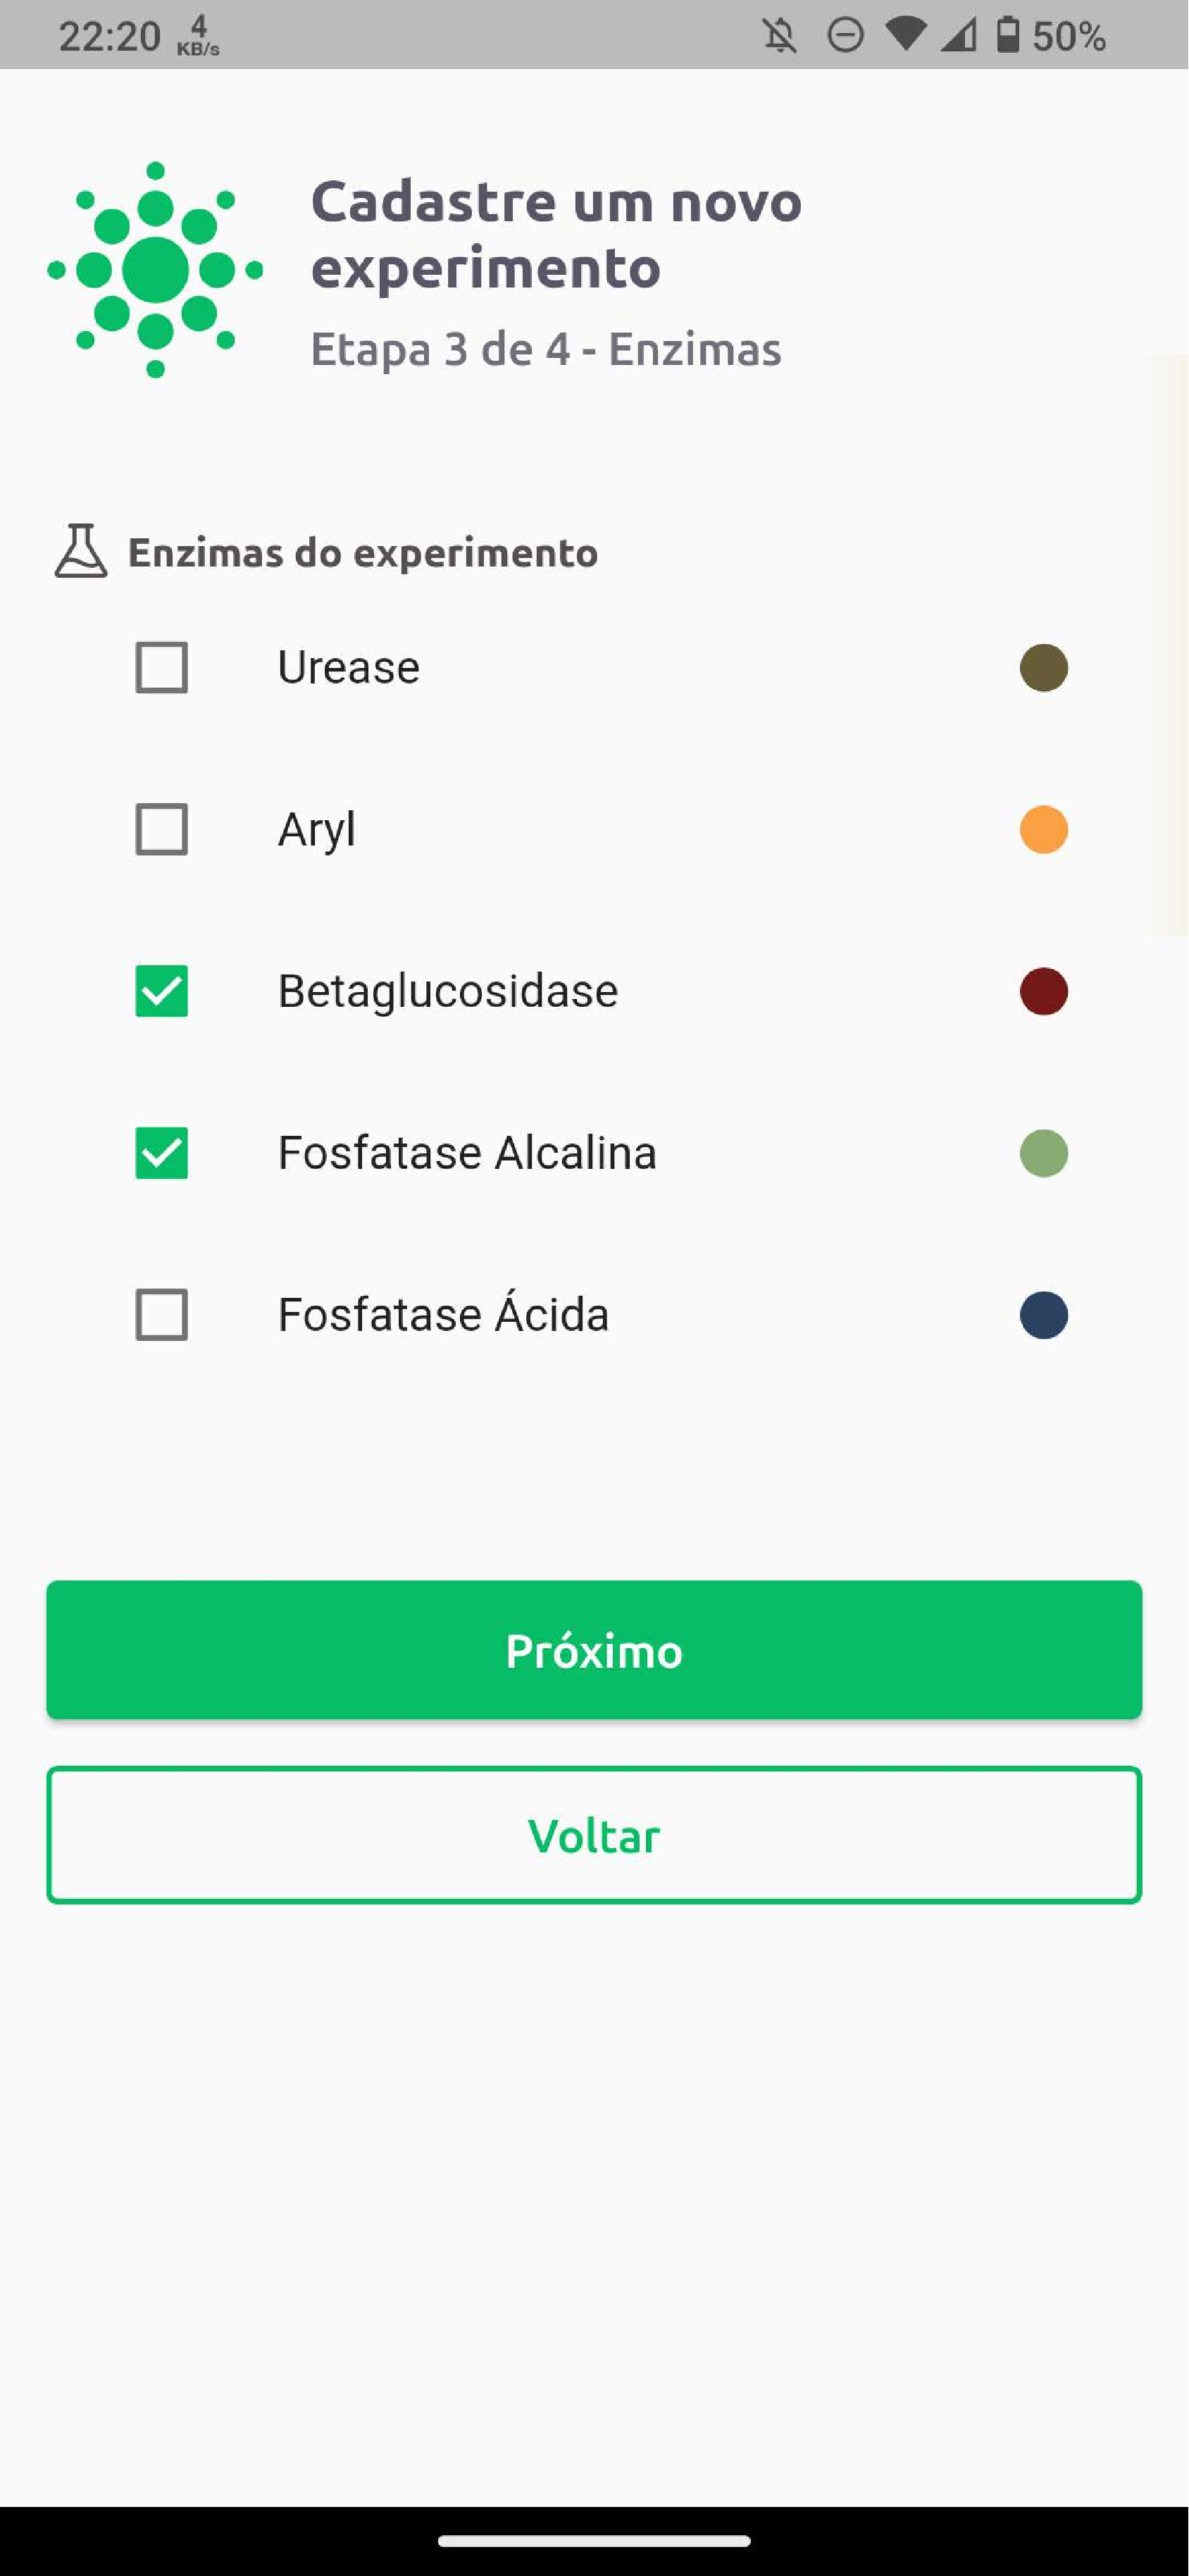
\includegraphics[width=.3\textwidth]{images/enzitech/cria_exp_3.pdf}
  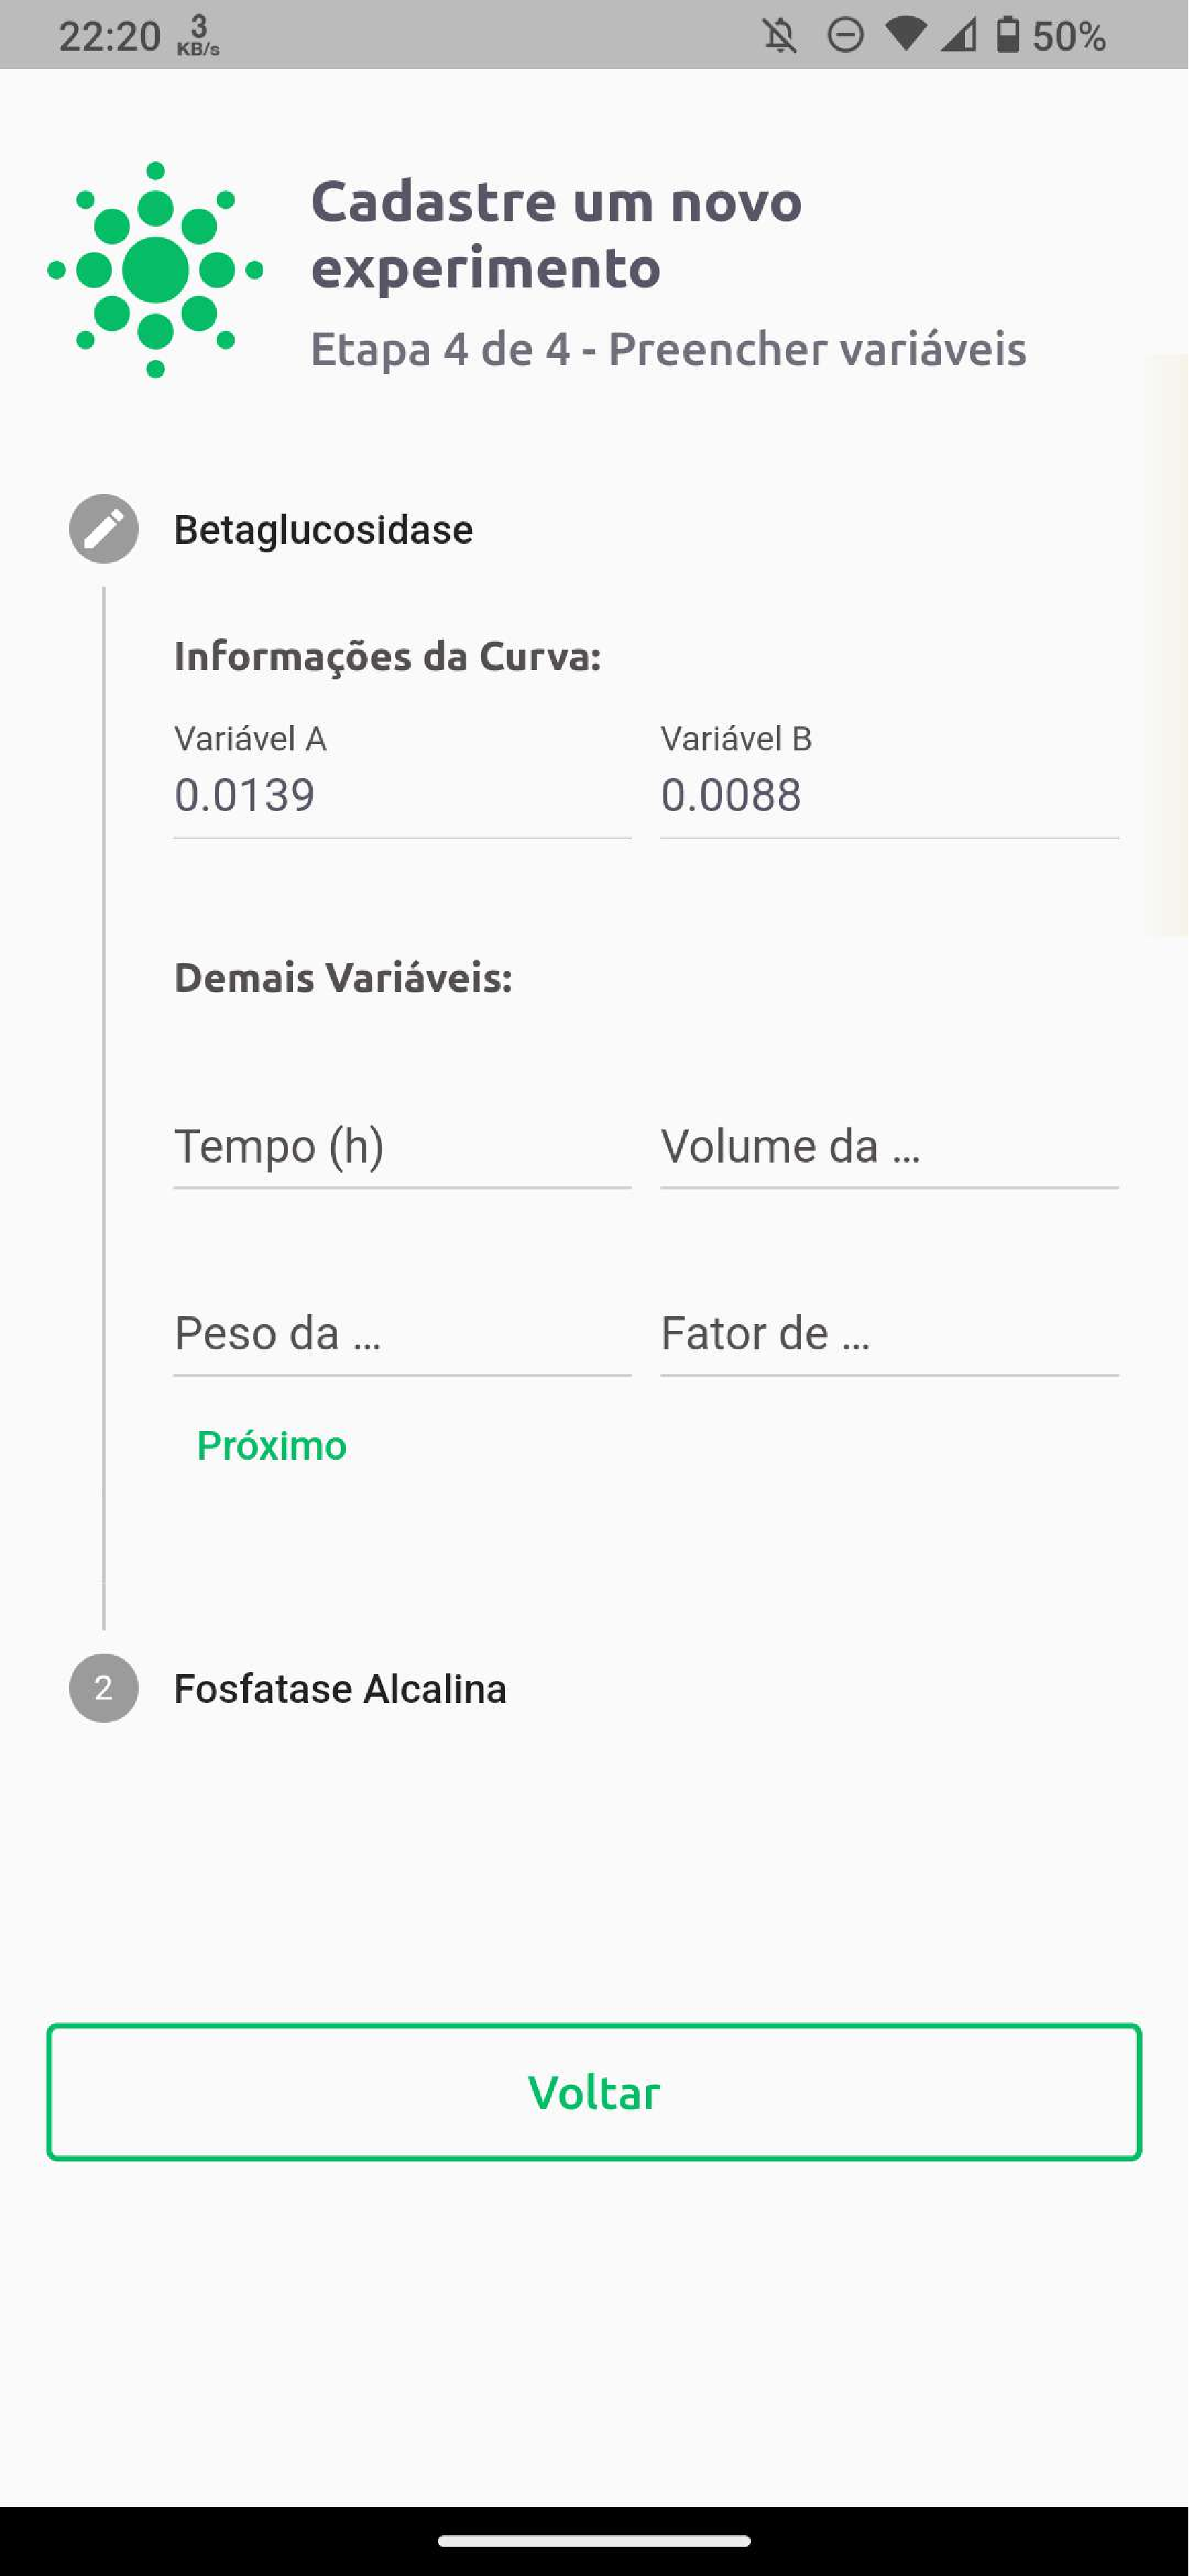
\includegraphics[width=.3\textwidth]{images/enzitech/cria_exp_4.pdf}
  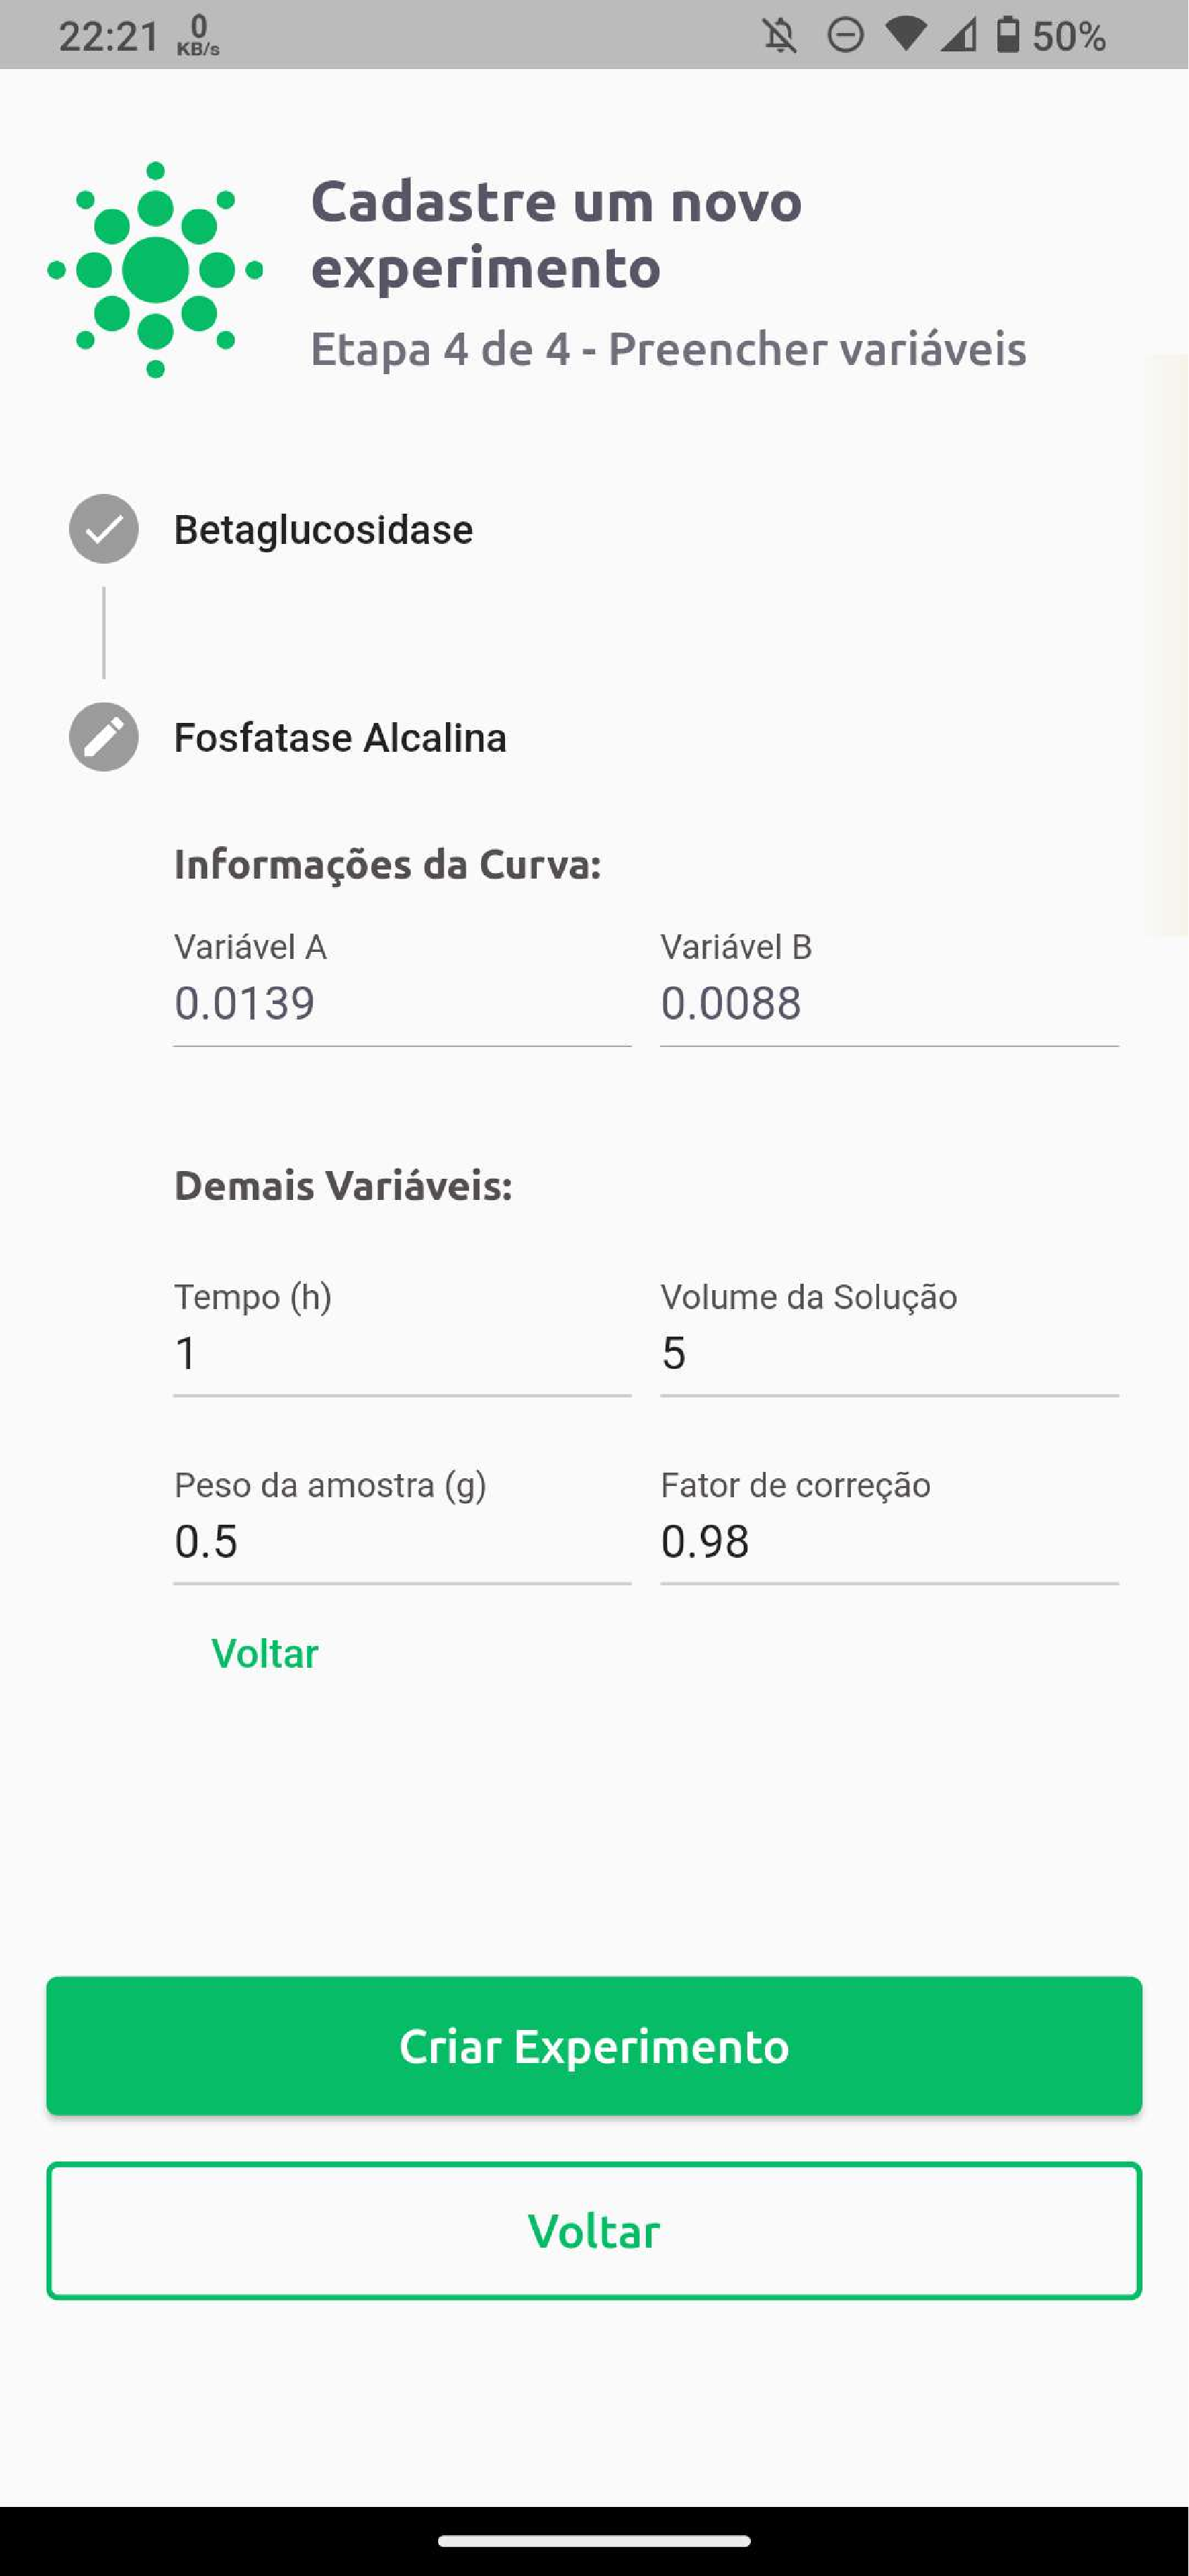
\includegraphics[width=.3\textwidth]{images/enzitech/cria_exp_5.pdf}

  \caption{Fluxo de criação de um experimento.}
  \label{fig:fluxo_cria_experimento}
  \acsfont{Fonte: Aplicativo Enzitech desenvolvido pelo autor}
  
\end{figure}


É possível ver na primeira imagem, na tela de experimentos, o filtro de "experimentos concluídos" aplicado, seguindo o fluxo, na segunda imagem é solicitada as informações de identificação do experimento, nome e descrição, a seguir, os tratamentos daquele experimento e quantas repetições serão realizadas, logo após, surge o seletor de enzimas, na quarta imagem (terceira etapa do processo de criação de experimento), nele é possível escolher quais enzimas farão parte do experimento, logo após surge a última etapa para o preenchimento dos valores variáveis daquele experimento, após criado (concluindo o caso de uso UC07), o usuário é levado para a funcionalidade de visualizar o experimento, explicado na \figref{fig:fluxo_experimento_detalhado} a seguir.

\begin{figure}[p]
  \centering
  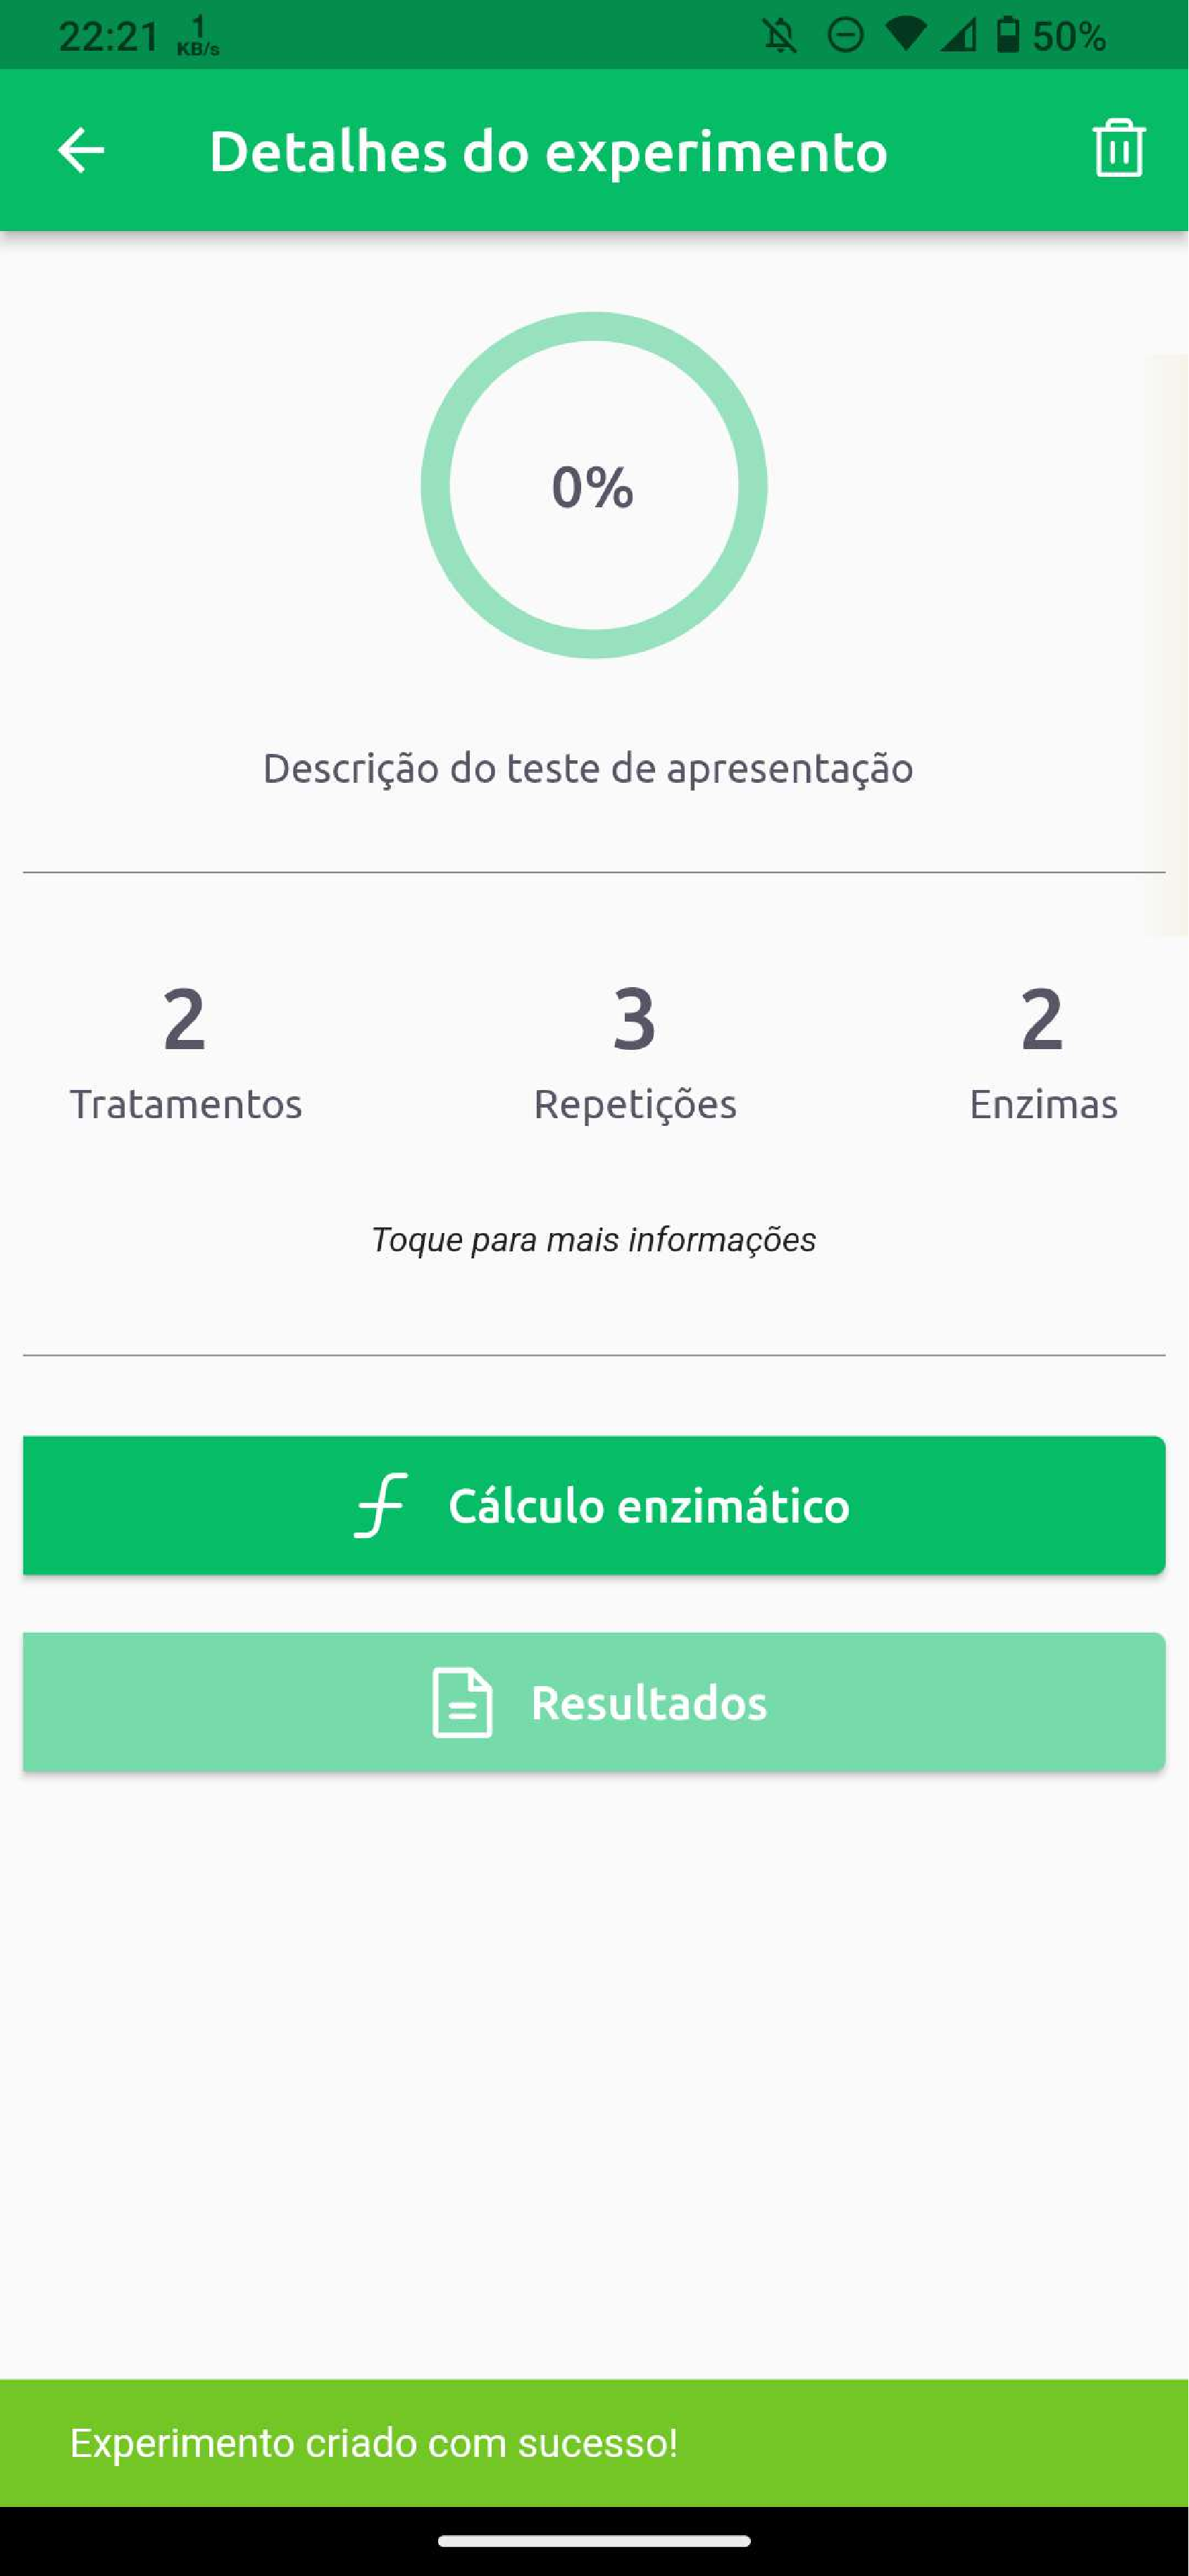
\includegraphics[width=.3\textwidth]{images/enzitech/exp_detalhado.pdf}
  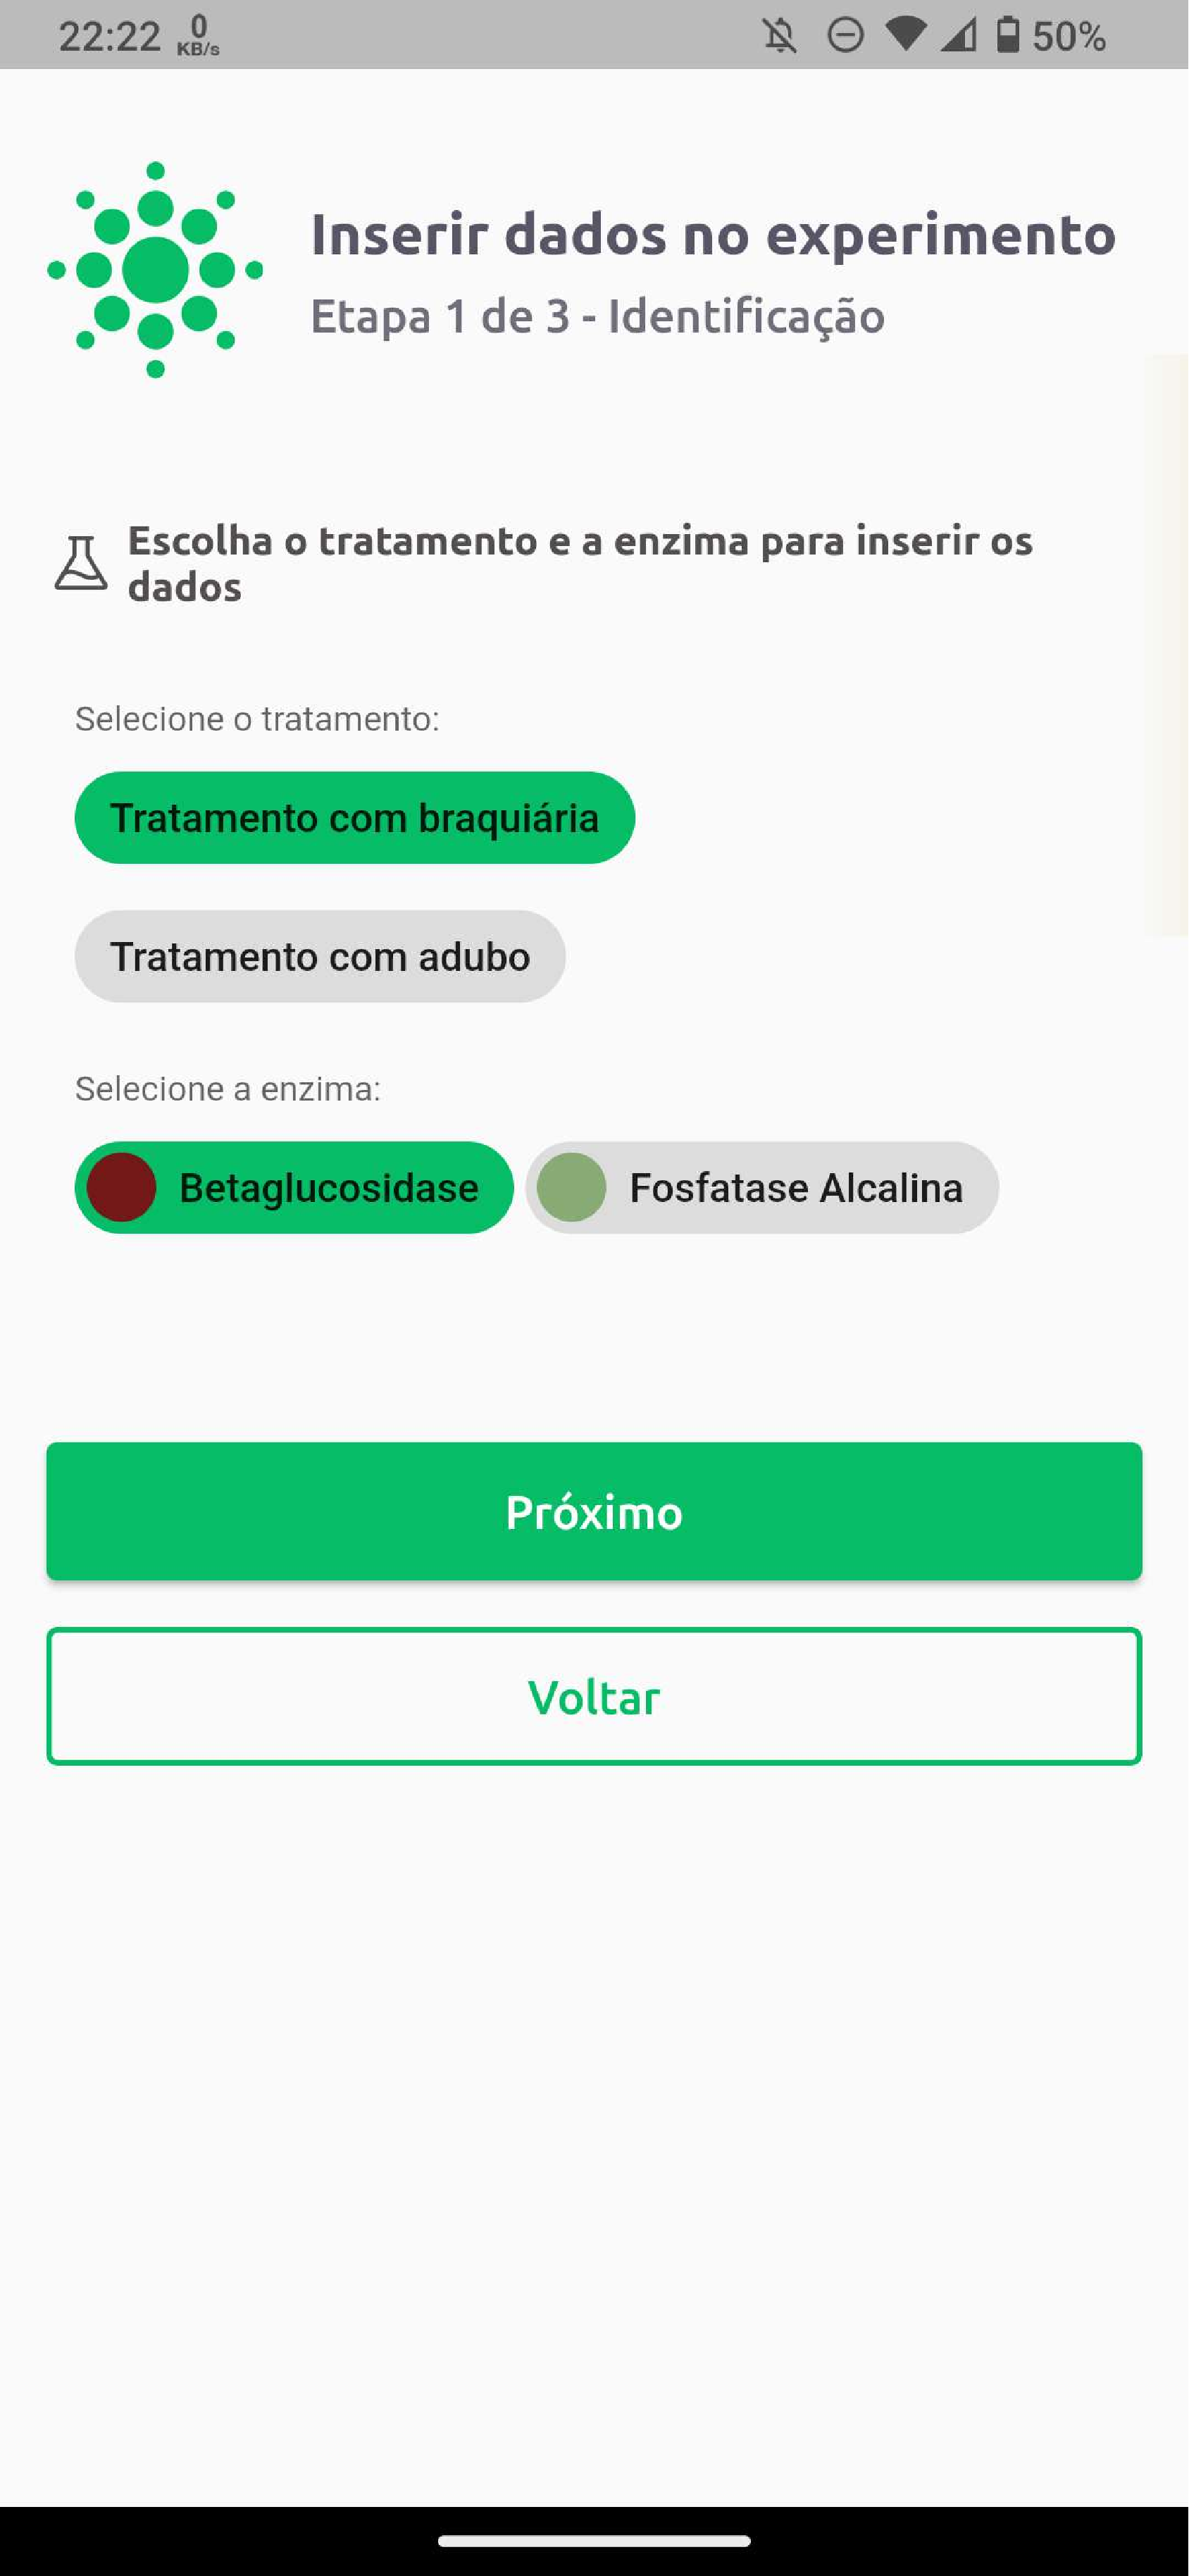
\includegraphics[width=.3\textwidth]{images/enzitech/calculo_1.pdf}
  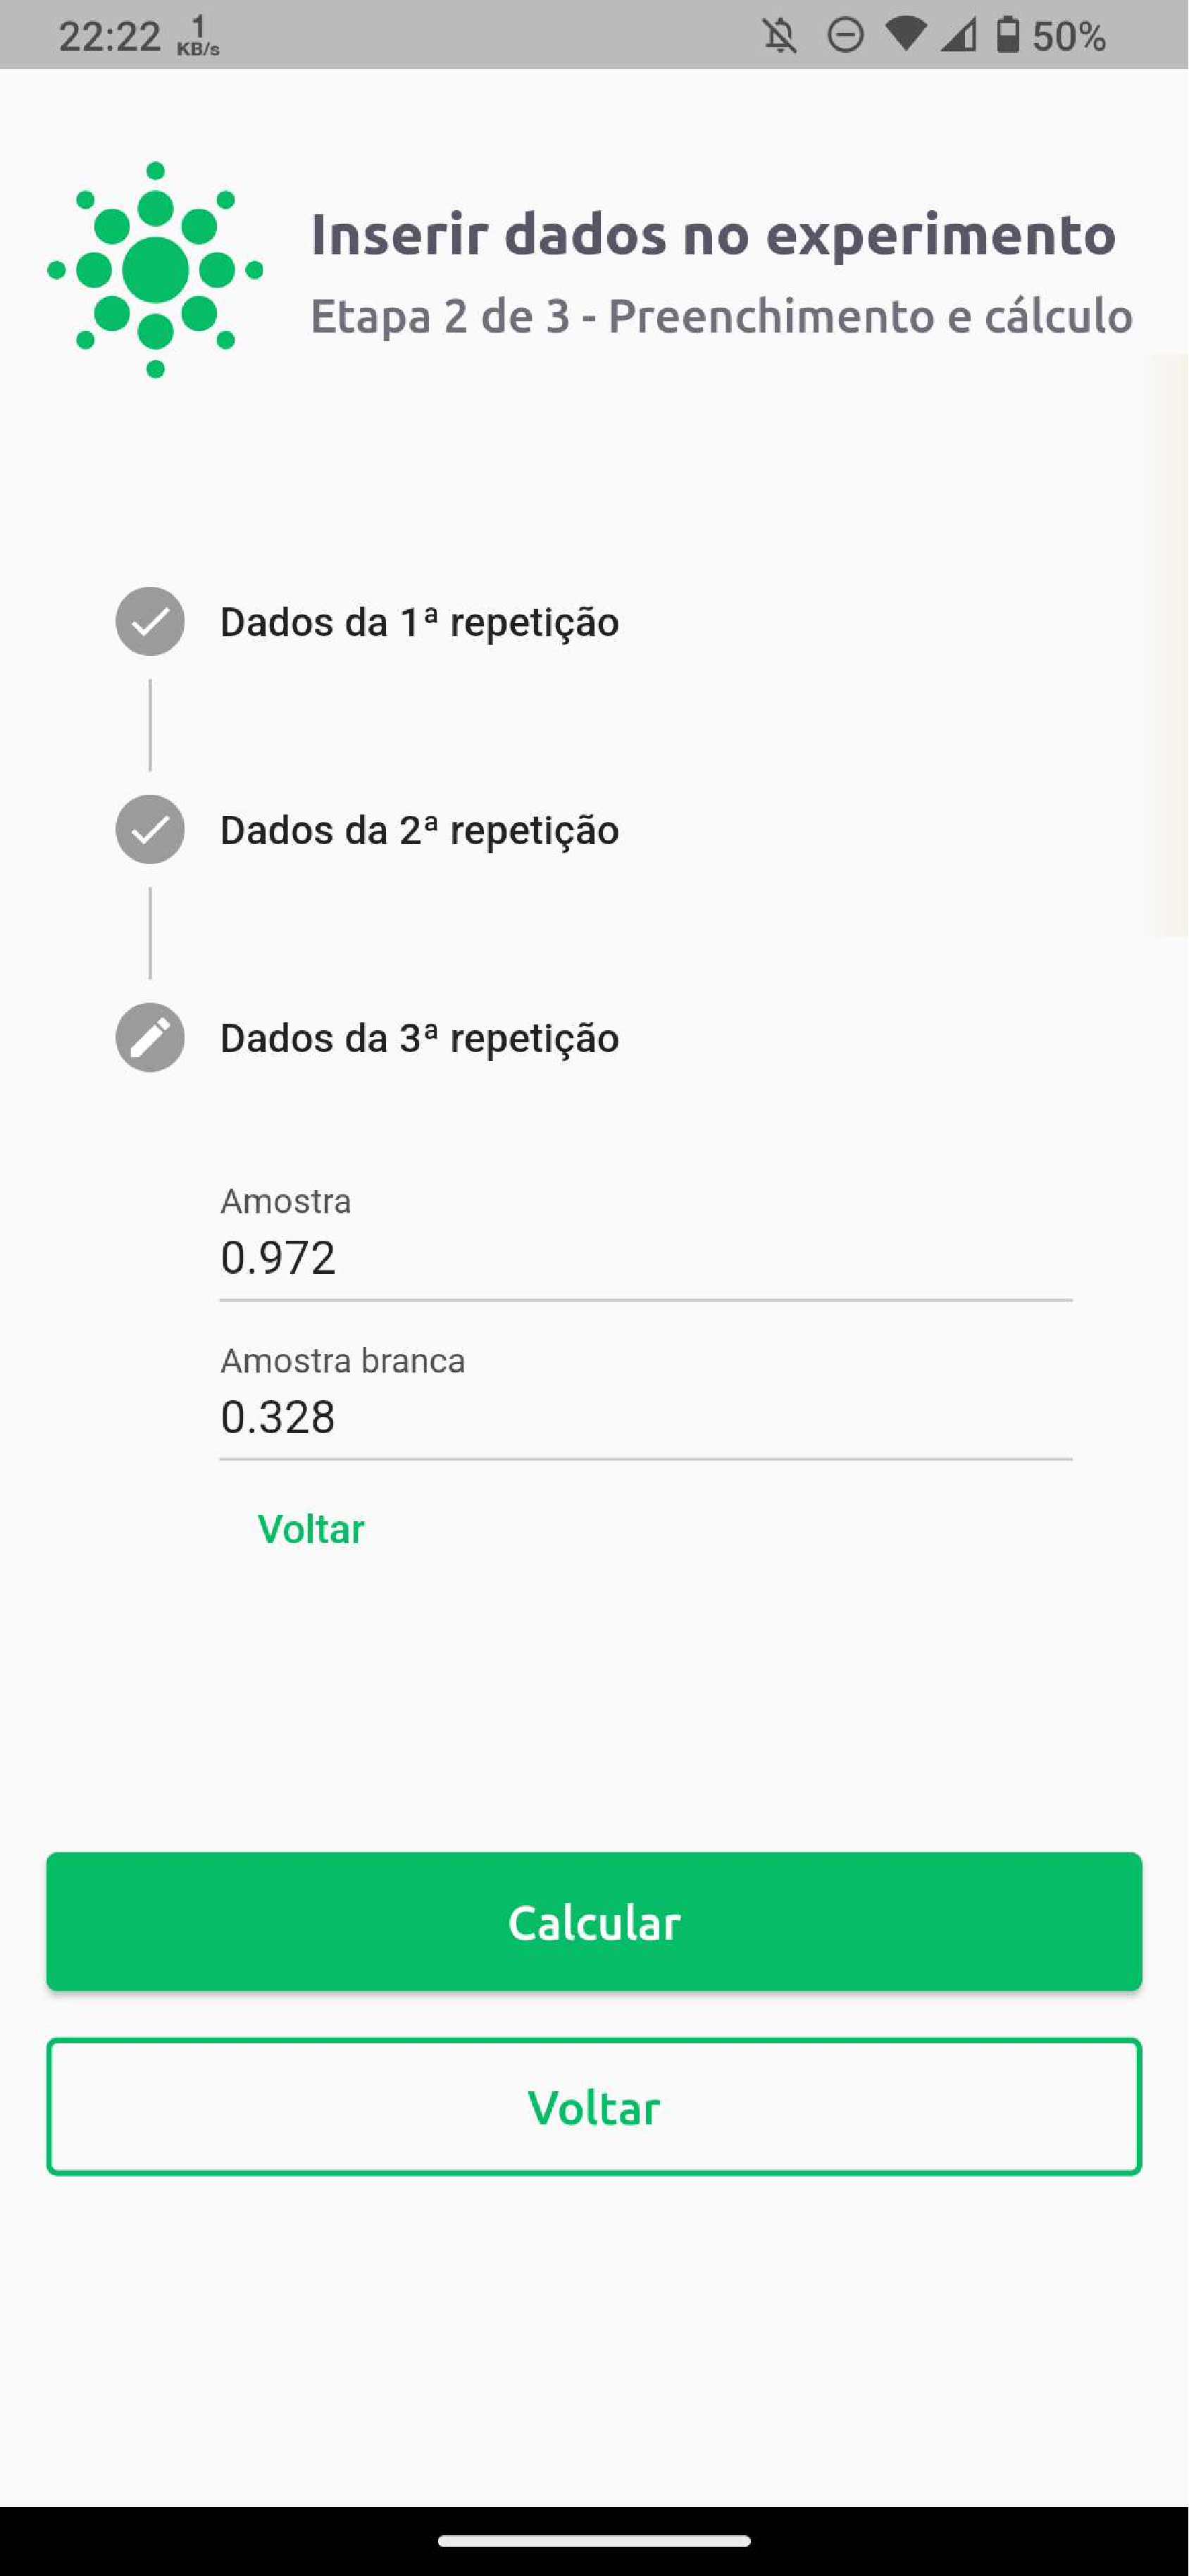
\includegraphics[width=.3\textwidth]{images/enzitech/calculo_2.pdf}

  \vspace{1cm}

  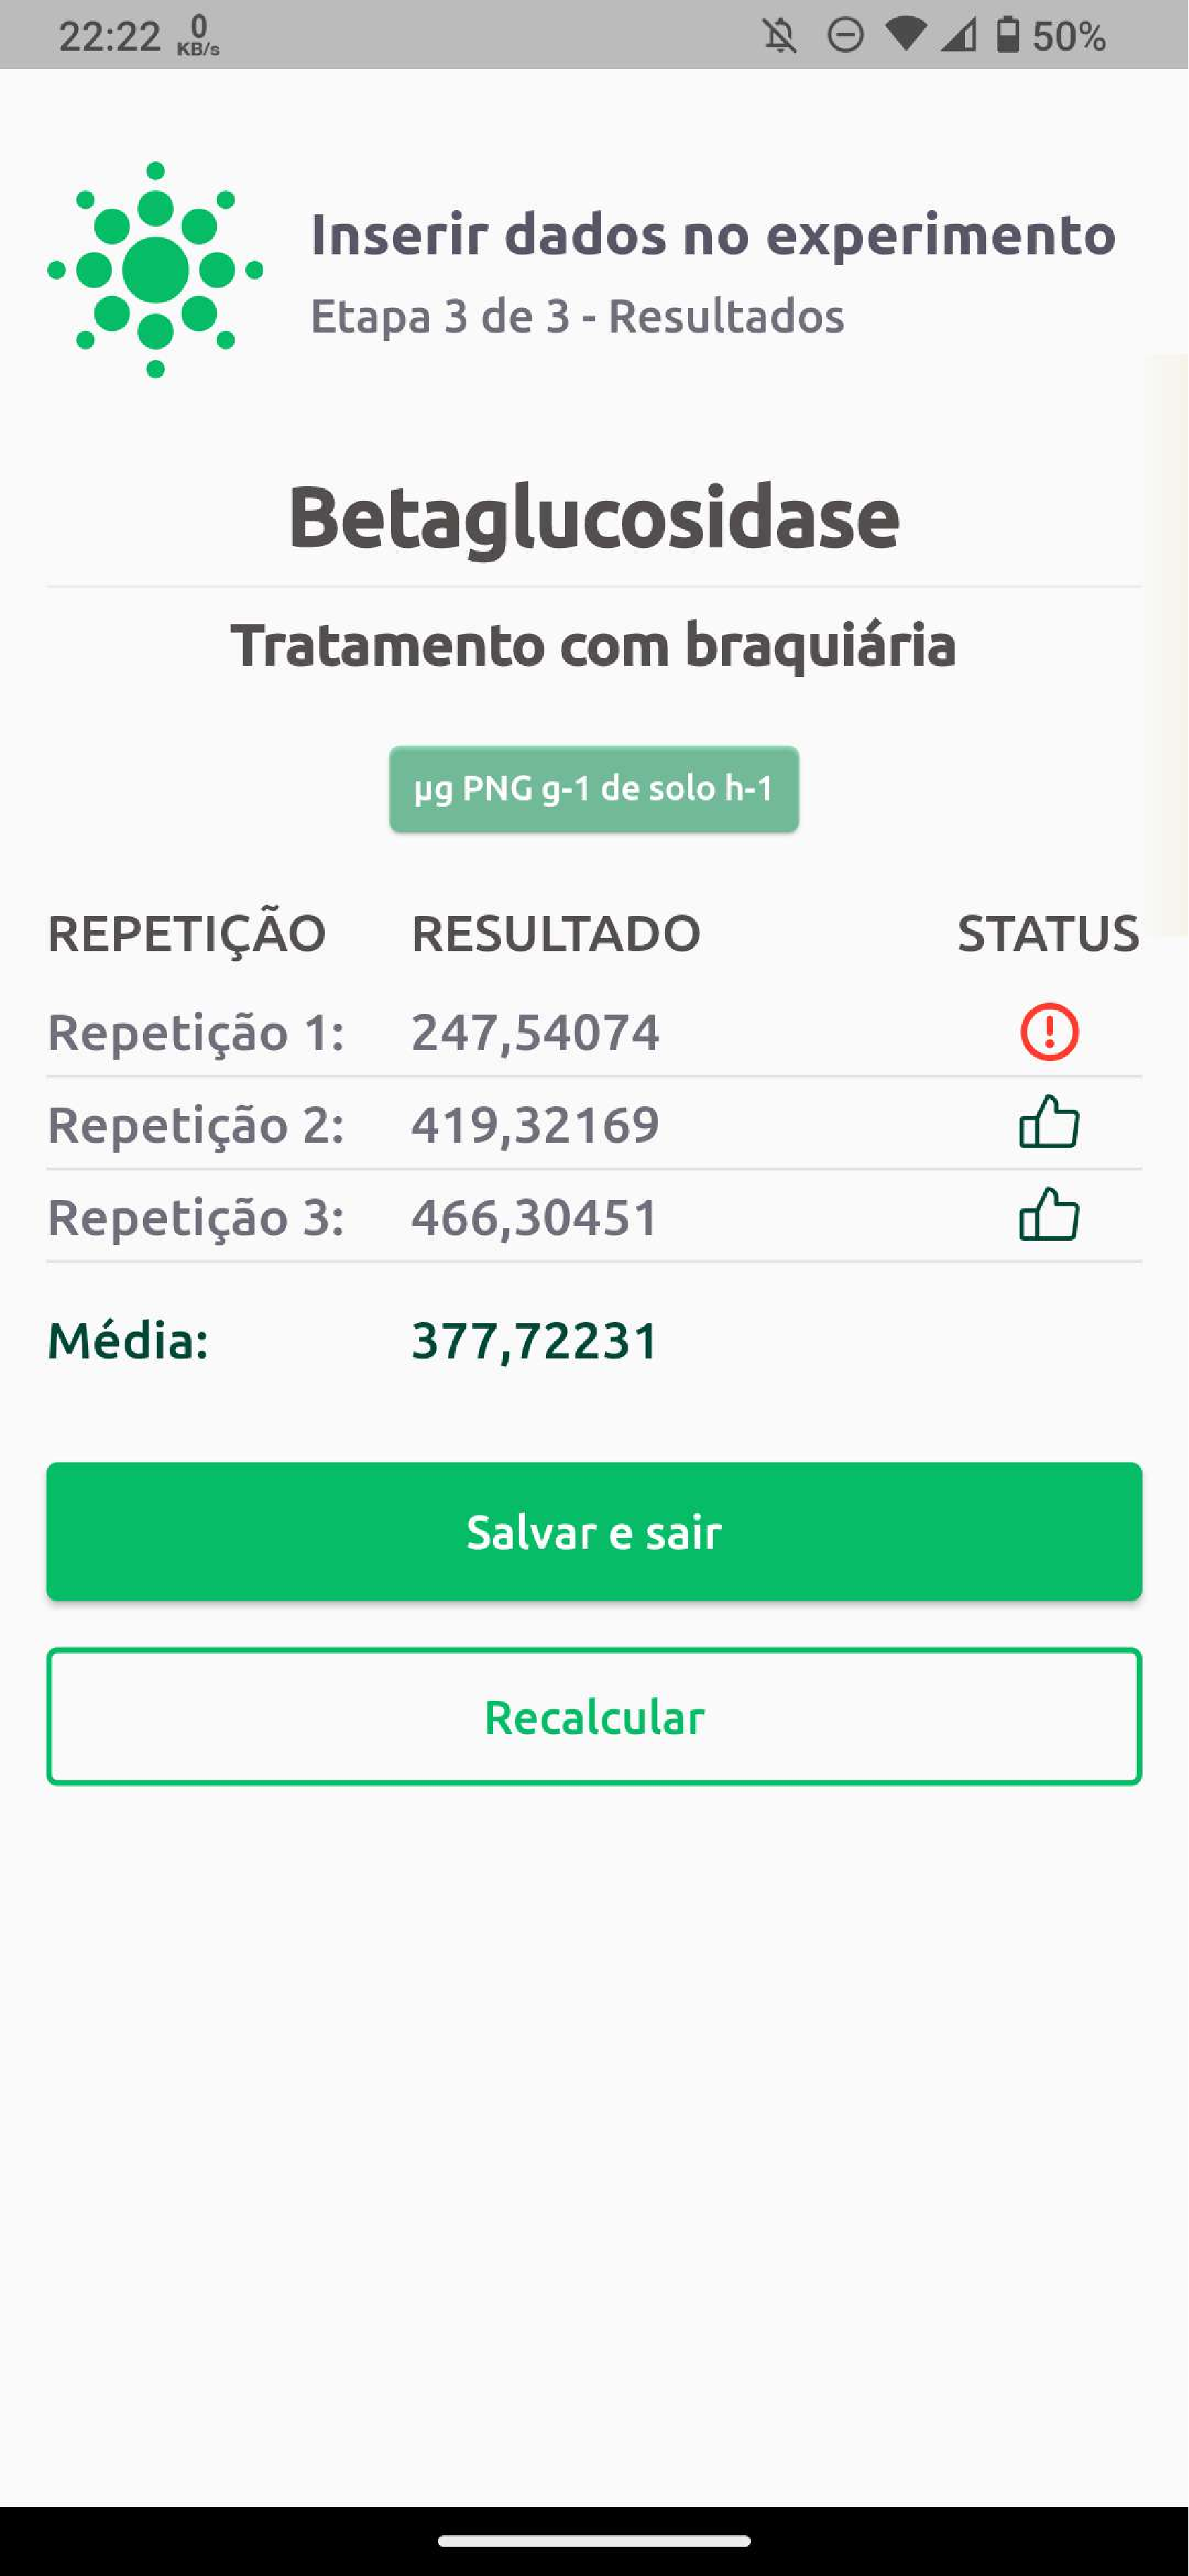
\includegraphics[width=.3\textwidth]{images/enzitech/calculo_3.pdf}
  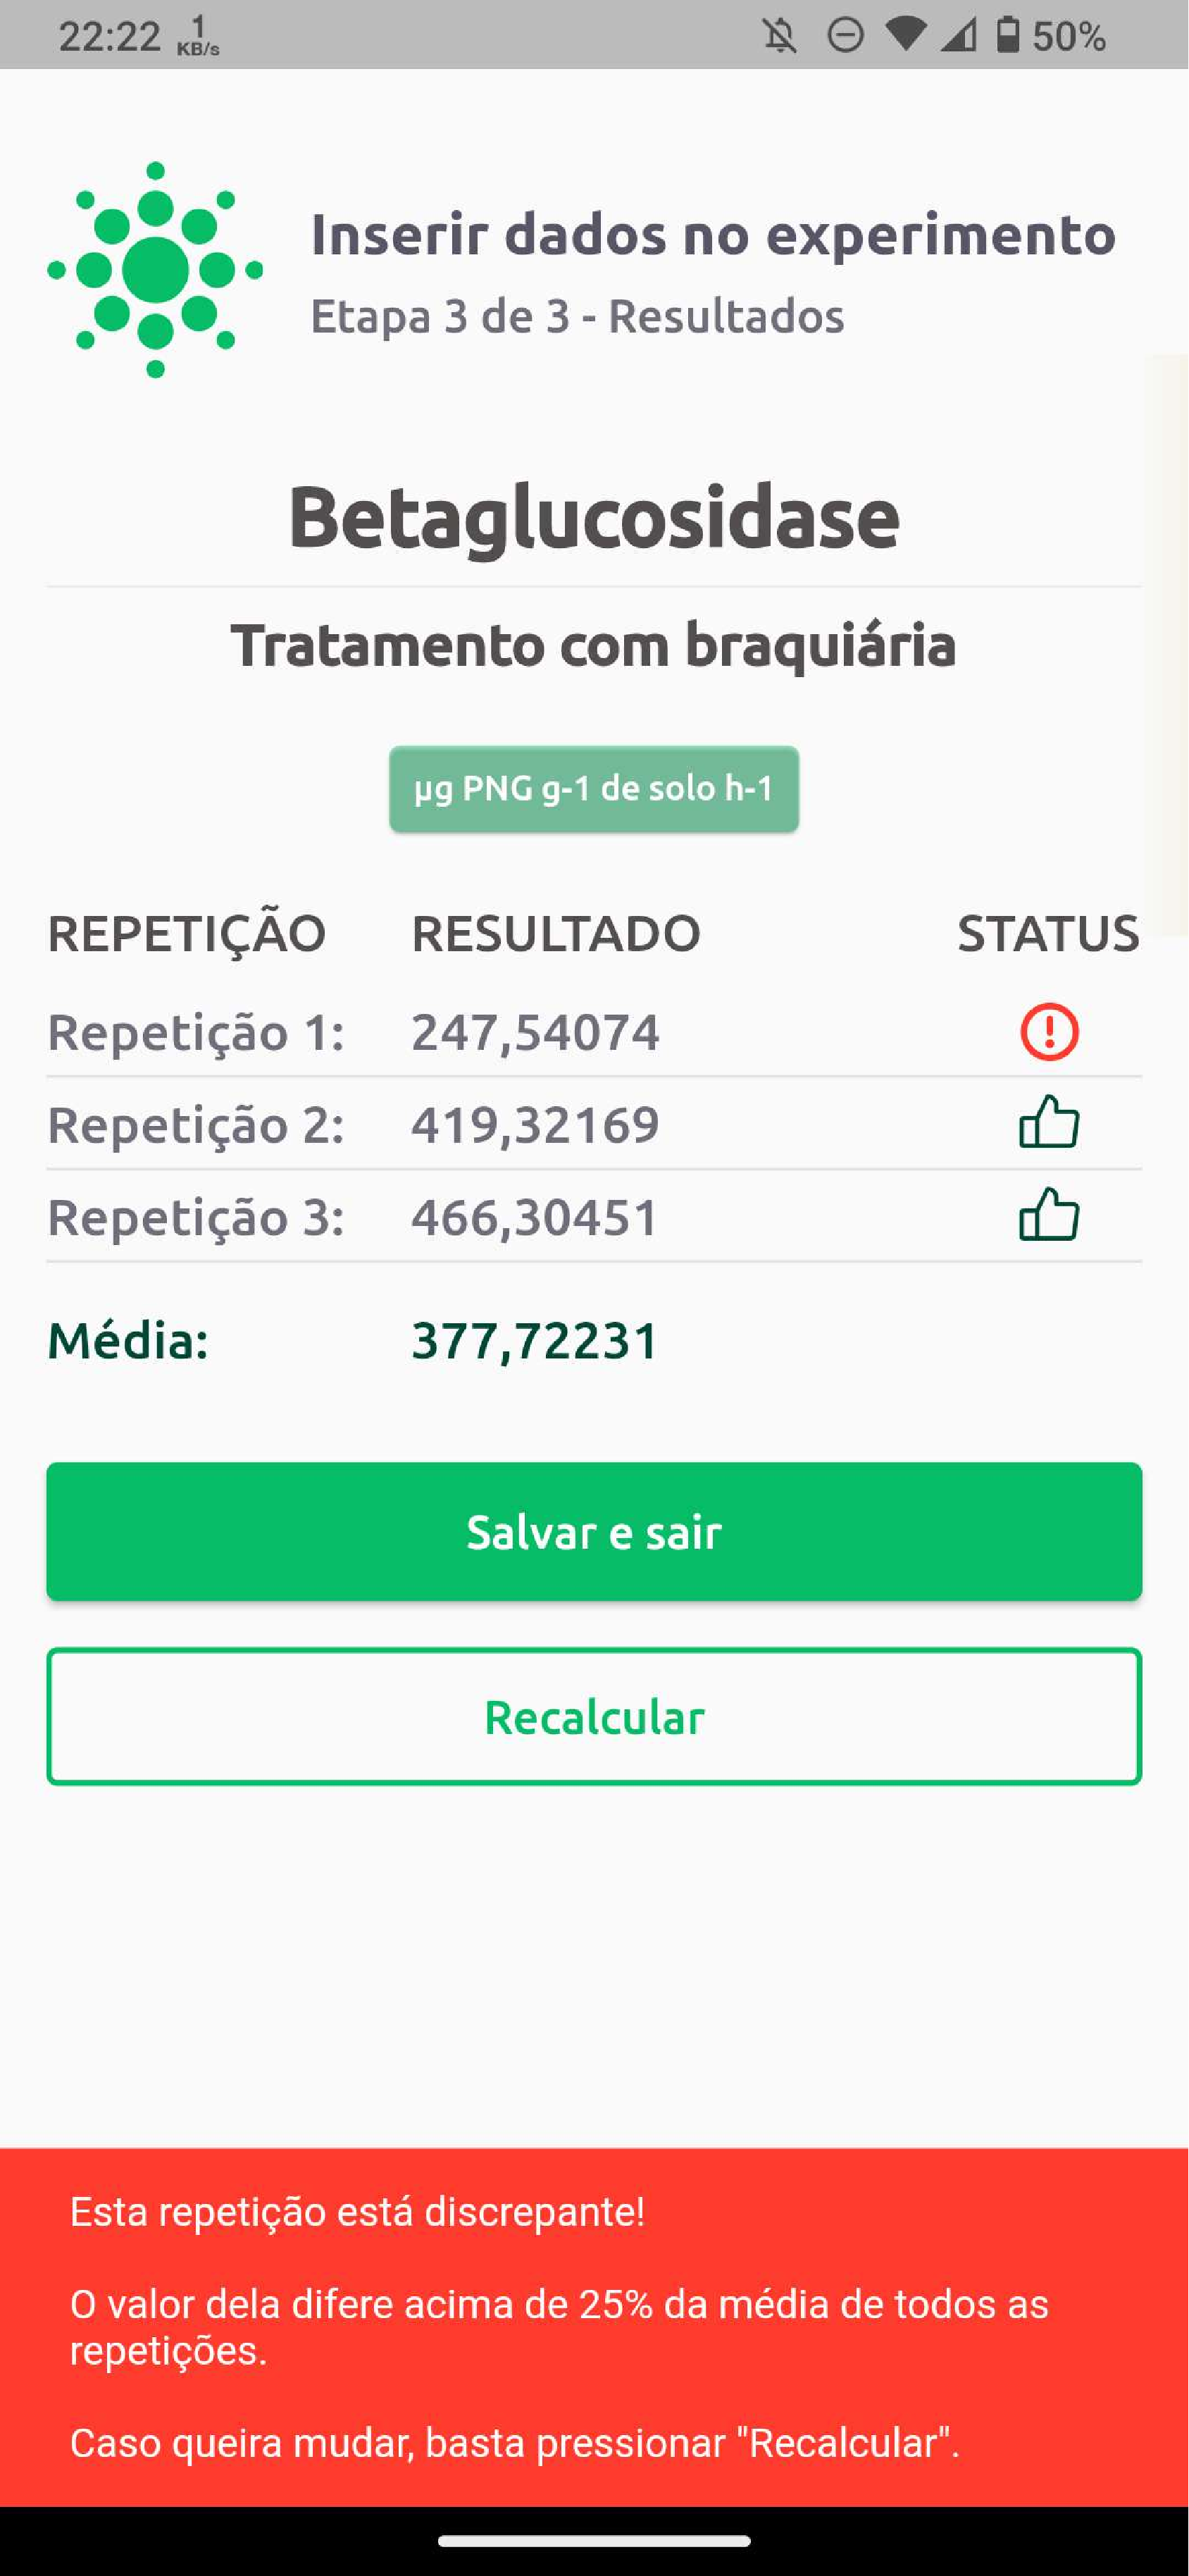
\includegraphics[width=.3\textwidth]{images/enzitech/calculo_4.pdf}
  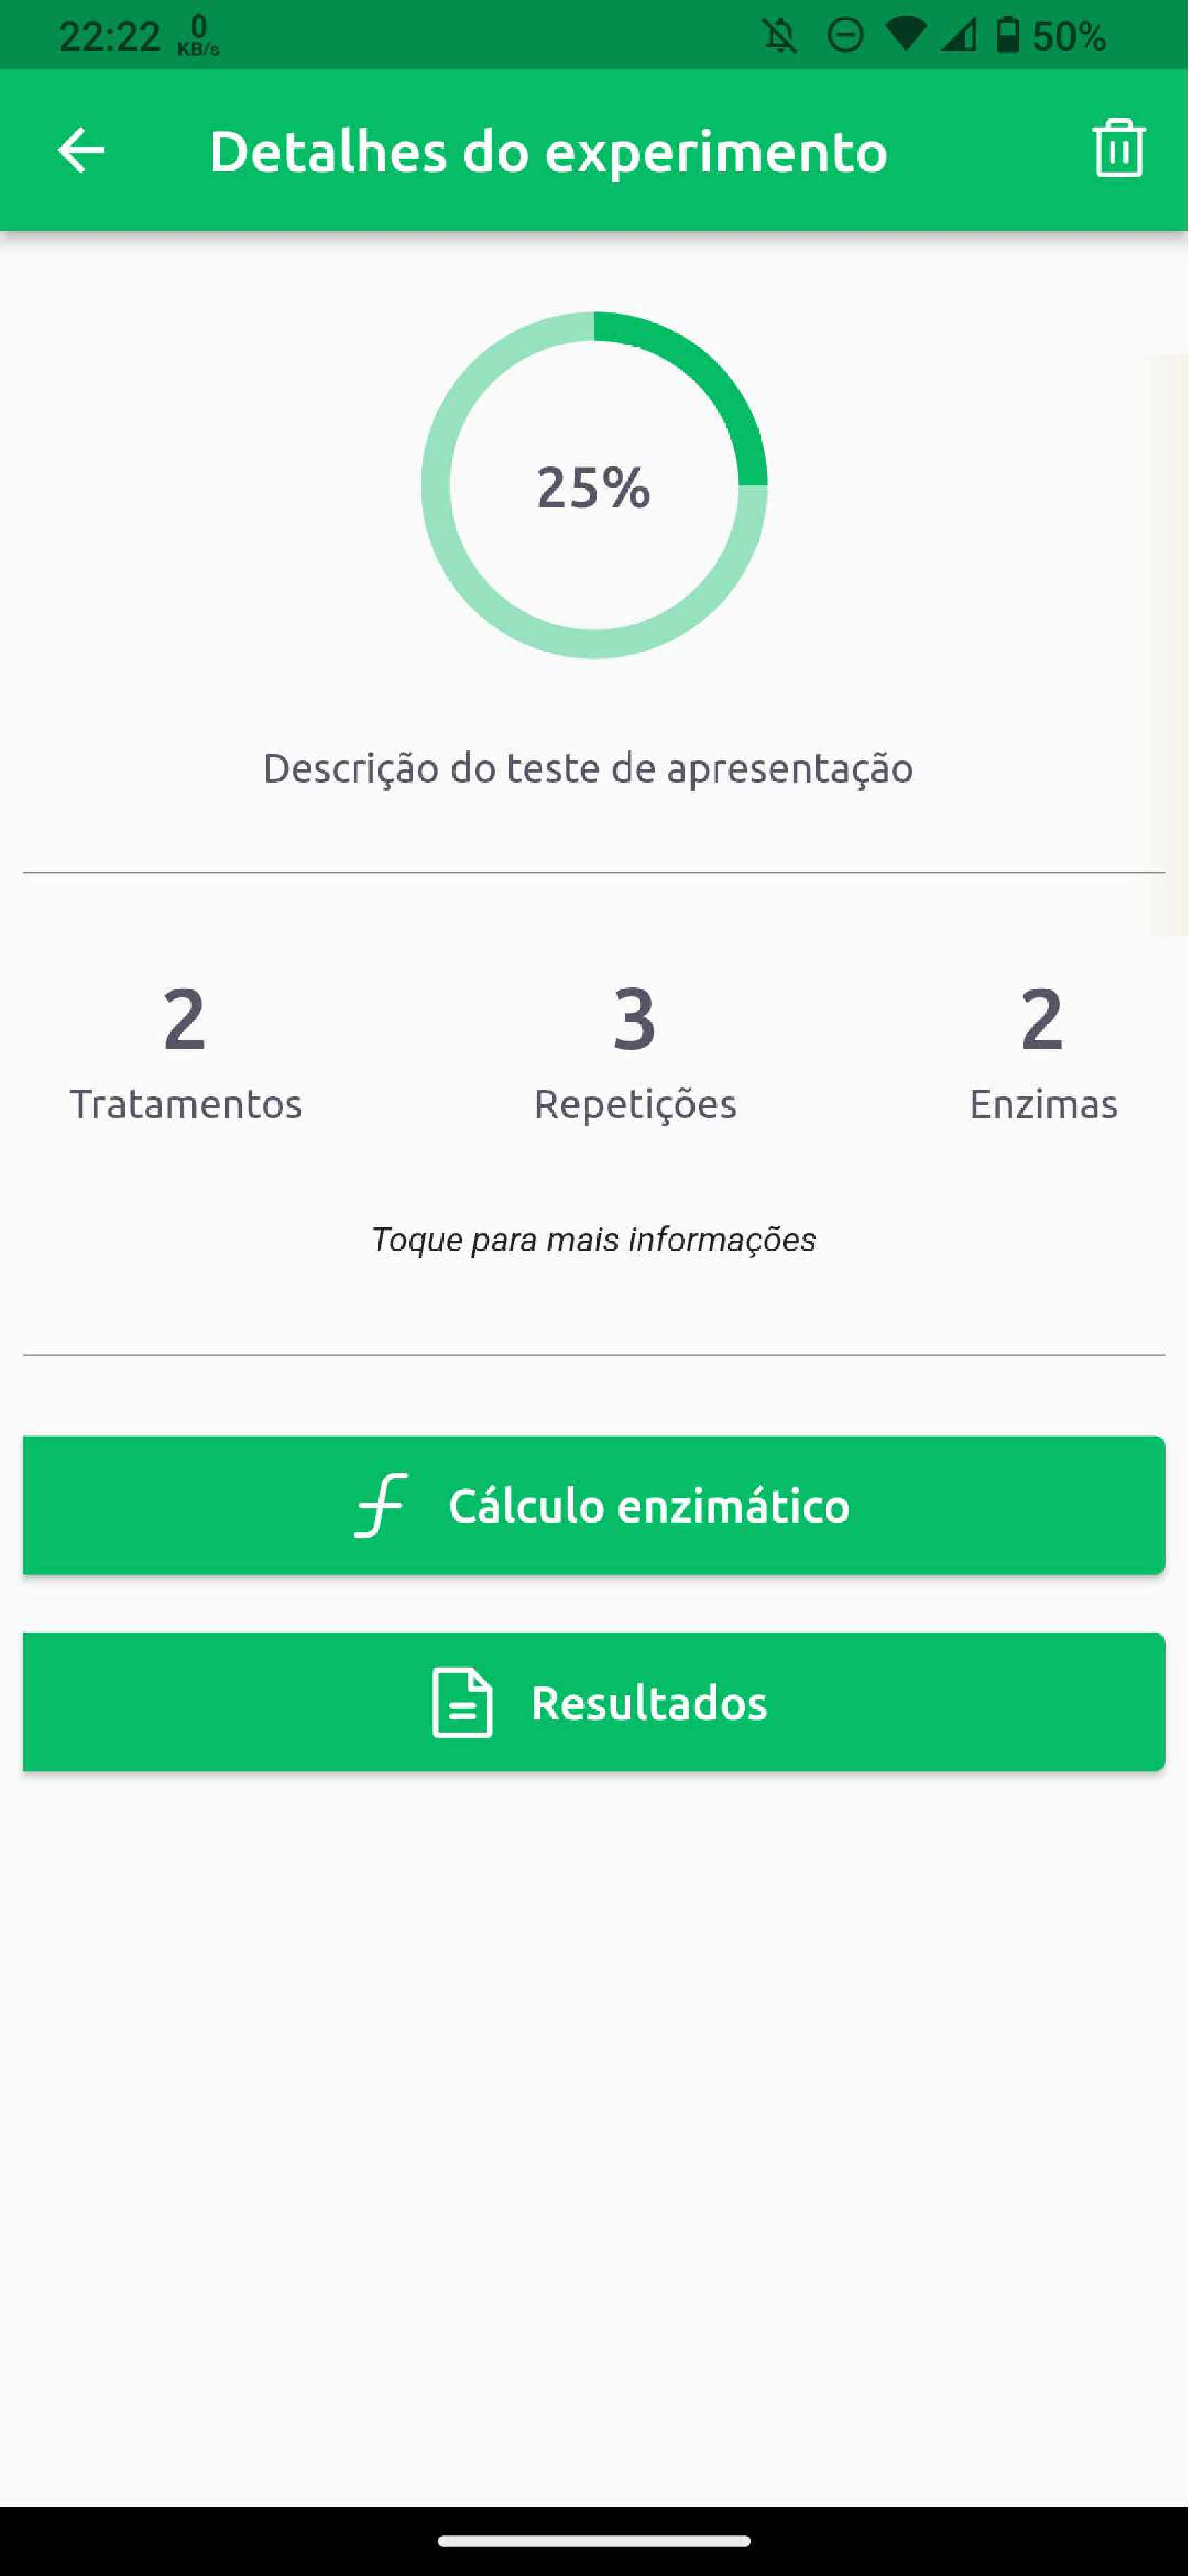
\includegraphics[width=.3\textwidth]{images/enzitech/exp_detalhado2.pdf}

  \caption{Fluxo de detalhamento e cálculo enzimático de um experimento.}
  \label{fig:fluxo_experimento_detalhado}
  \acsfont{Fonte: Aplicativo Enzitech desenvolvido pelo autor}
  
\end{figure}

Após o experimento criado, o usuário pode ver seus detalhes, como a quantidade de enzimas, tratamentos e repetições, seu progresso (caso de uso UC08) e a possibilidade de excluí-lo, além disso, o acesso à outras duas funcionalidades, a de cálculo enzimático, para inserção de dados no experimento, e a de resultados, para a visualização e compartilhamento desses dados.

Acompanhando a \figref{fig:fluxo_experimento_detalhado}, para o preenchimento do experimento é necessário escolher um tratamento e uma enzima, assim, gerando um conjunto de informações para prosseguir com a inserção dos valores em suas respectivas repetições.

Após todos os valores inseridos, o usuário clica em carregar e é levado para uma tela de resultados deste cálculo e a média (quarta e quinta imagem), nesta tela, é possível ver os resultados e receber um \textit{feedback} sobre a discrepância dos valores em comparação com a média de todos os resultados das repetições, assim, sendo possível perceber algum valor que pode estar inserido incorretamente, resultando em dados errôneos, desta forma, o usuário pode recalcular, corrigindo com novos valores ou prosseguir, salvando e saindo da tela de cálculo (caso de uso UC09).

Em seguida, quando um experimento já tem dados suficientes (progresso maior ou igual a 1\%), é possível ver e compartilhar os resultados obtidos (casos de uso UC10 e UC11), mostrados a seguir na \figref{fig:fluxo_resultados}.

\begin{figure}[p]
  \centering
  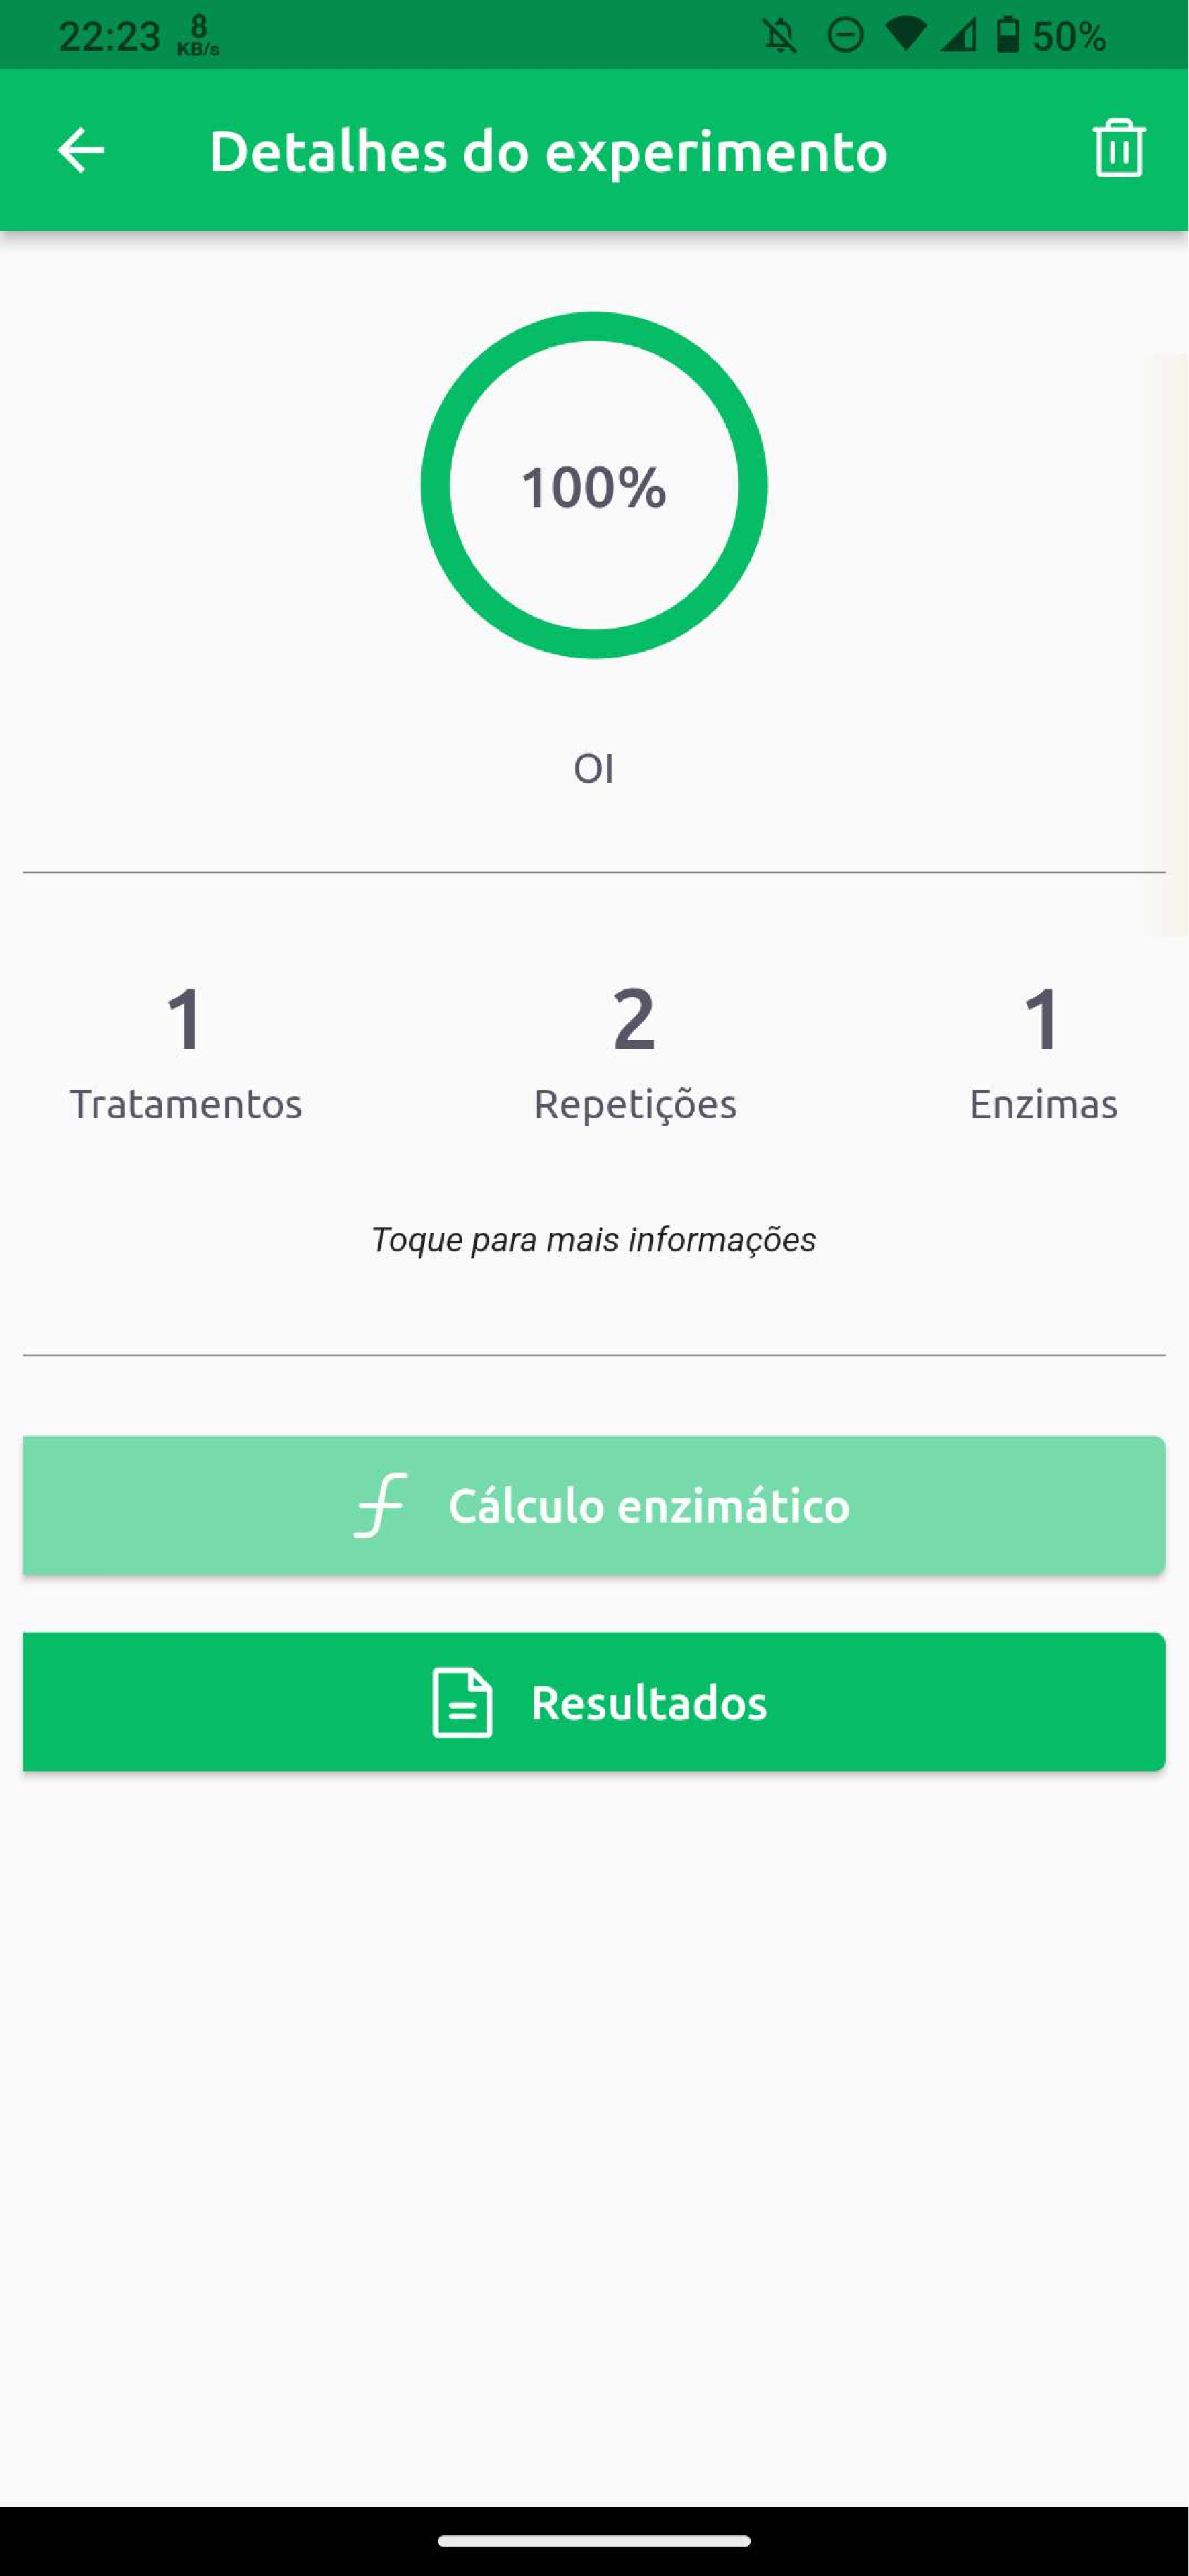
\includegraphics[width=.3\textwidth]{images/enzitech/exp_concluido.pdf}
  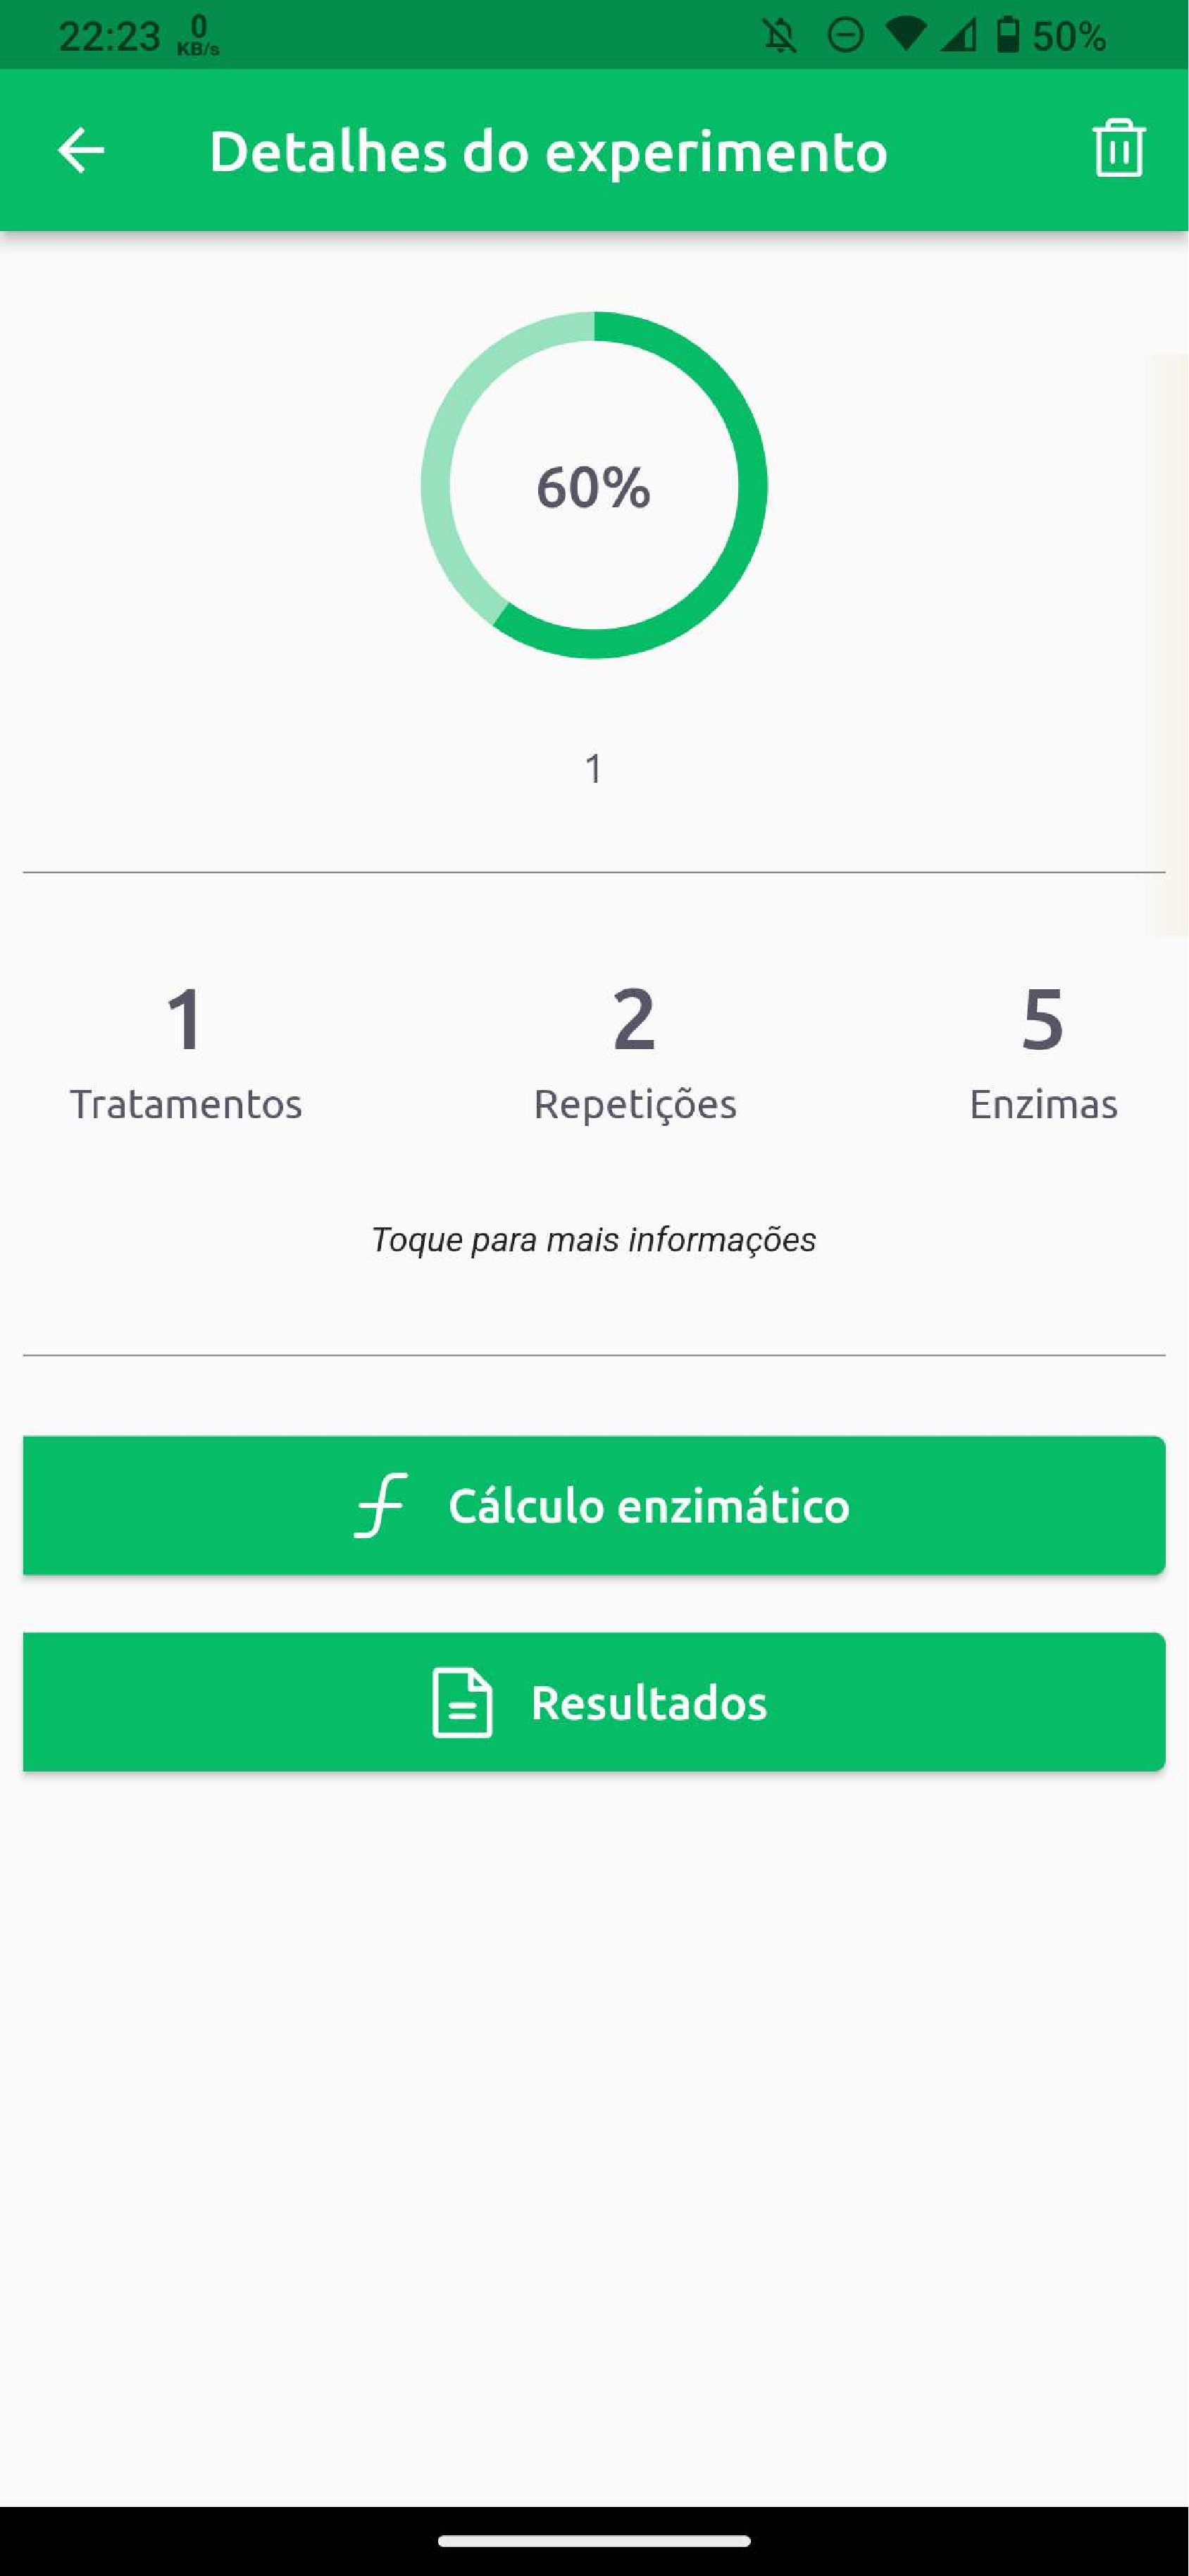
\includegraphics[width=.3\textwidth]{images/enzitech/exp_detalhado3.pdf}
  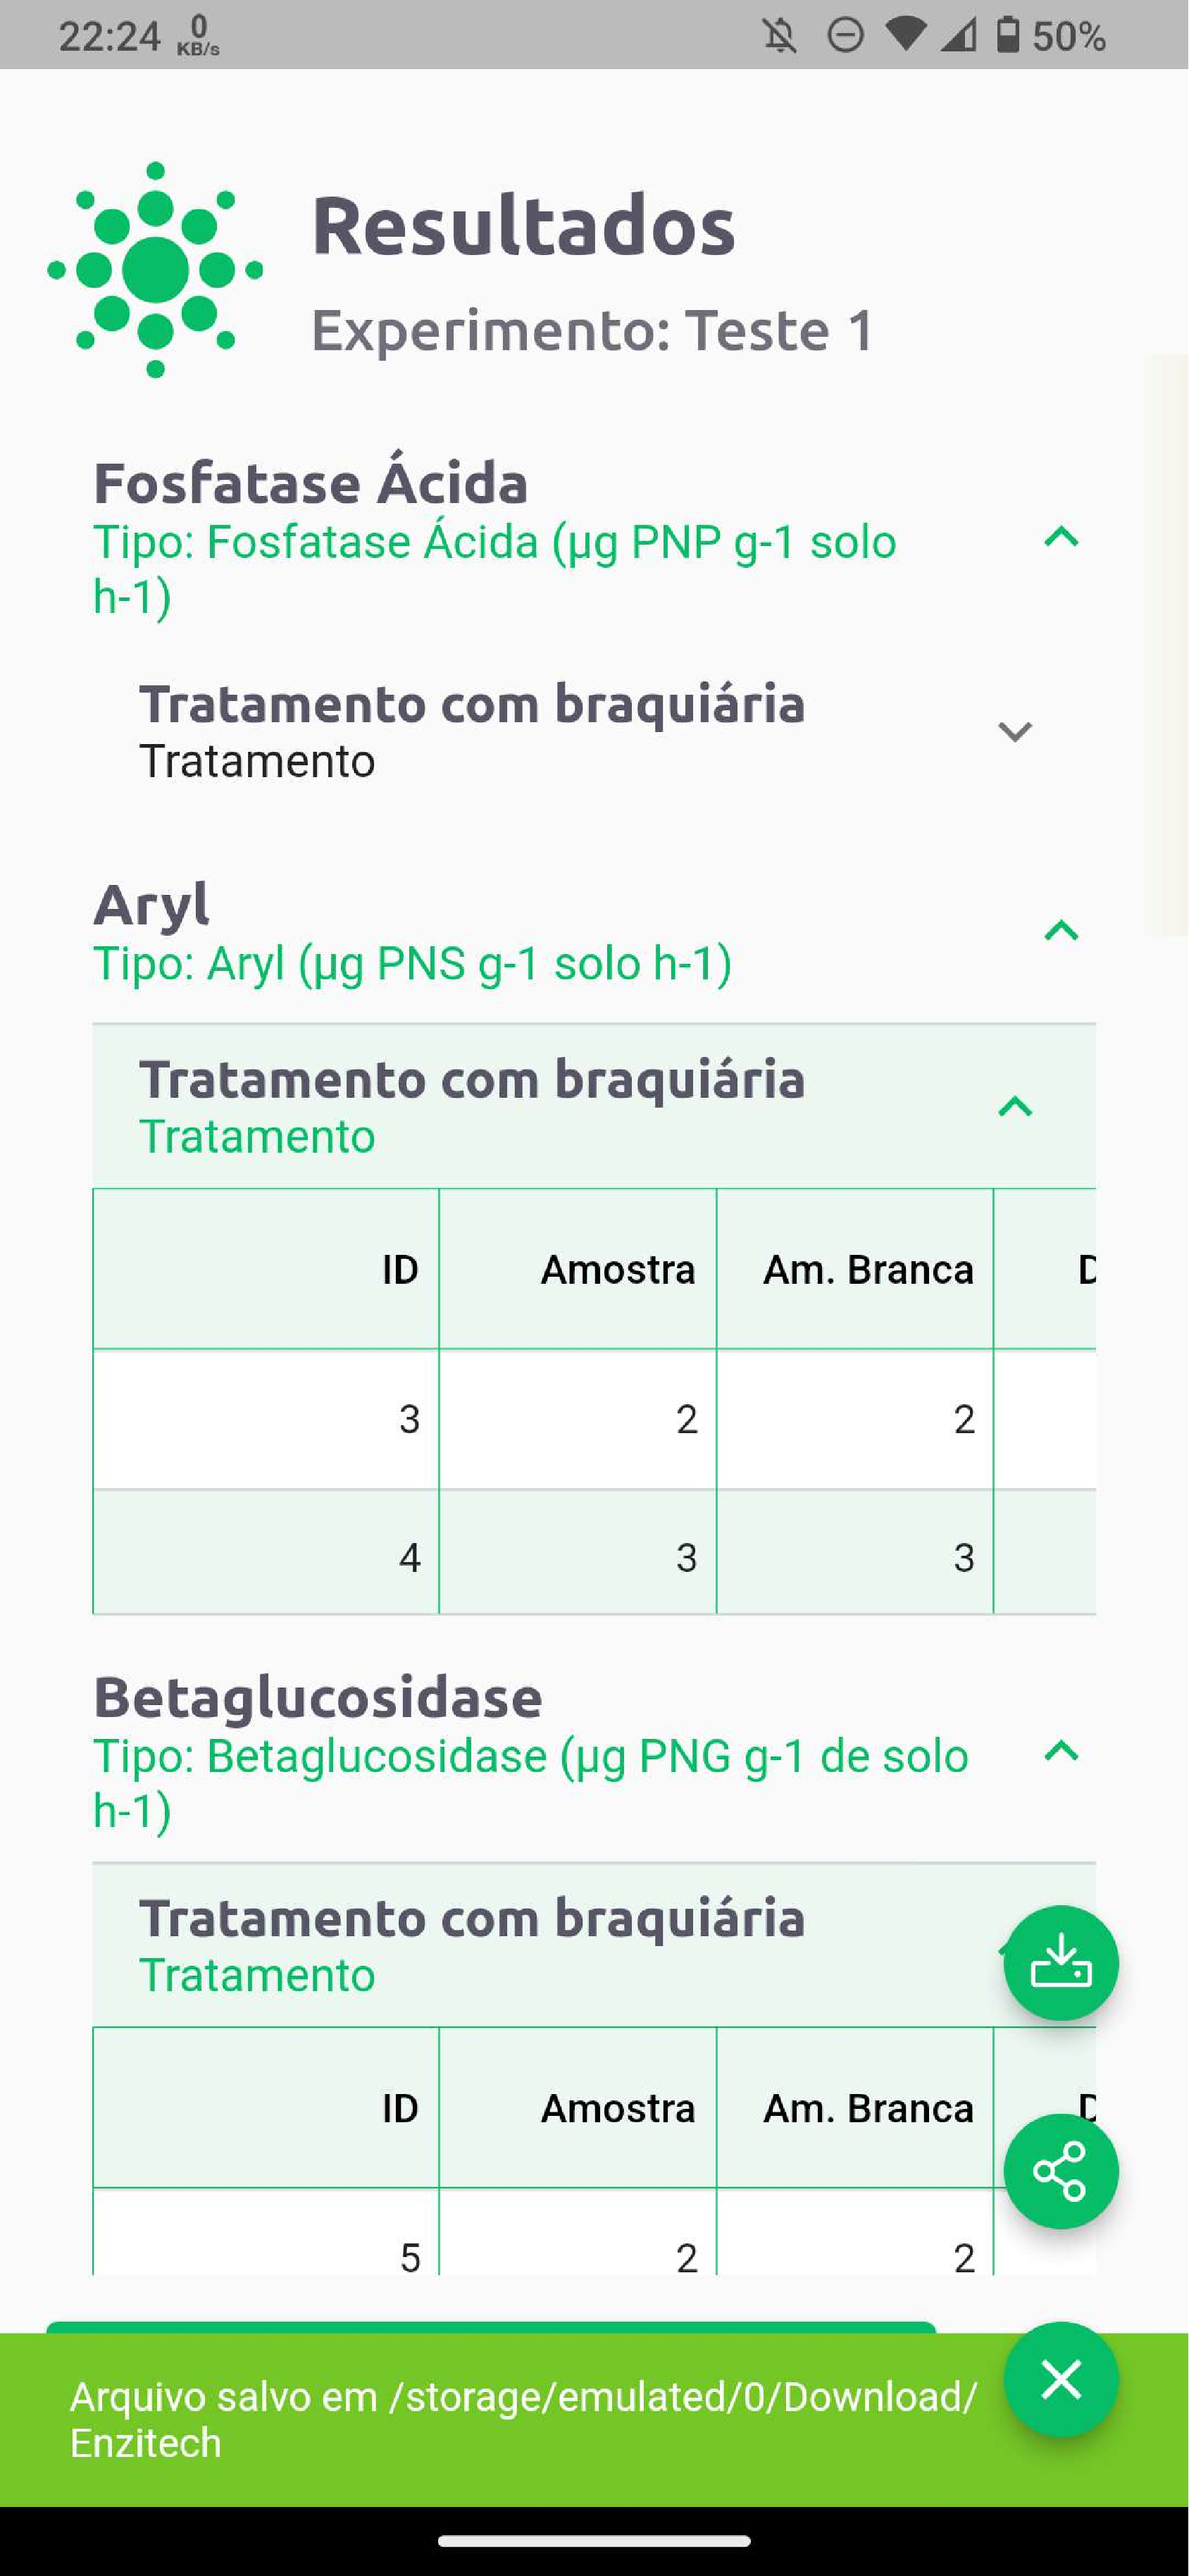
\includegraphics[width=.3\textwidth]{images/enzitech/resultados_salvar.pdf}

  \vspace{1cm}

  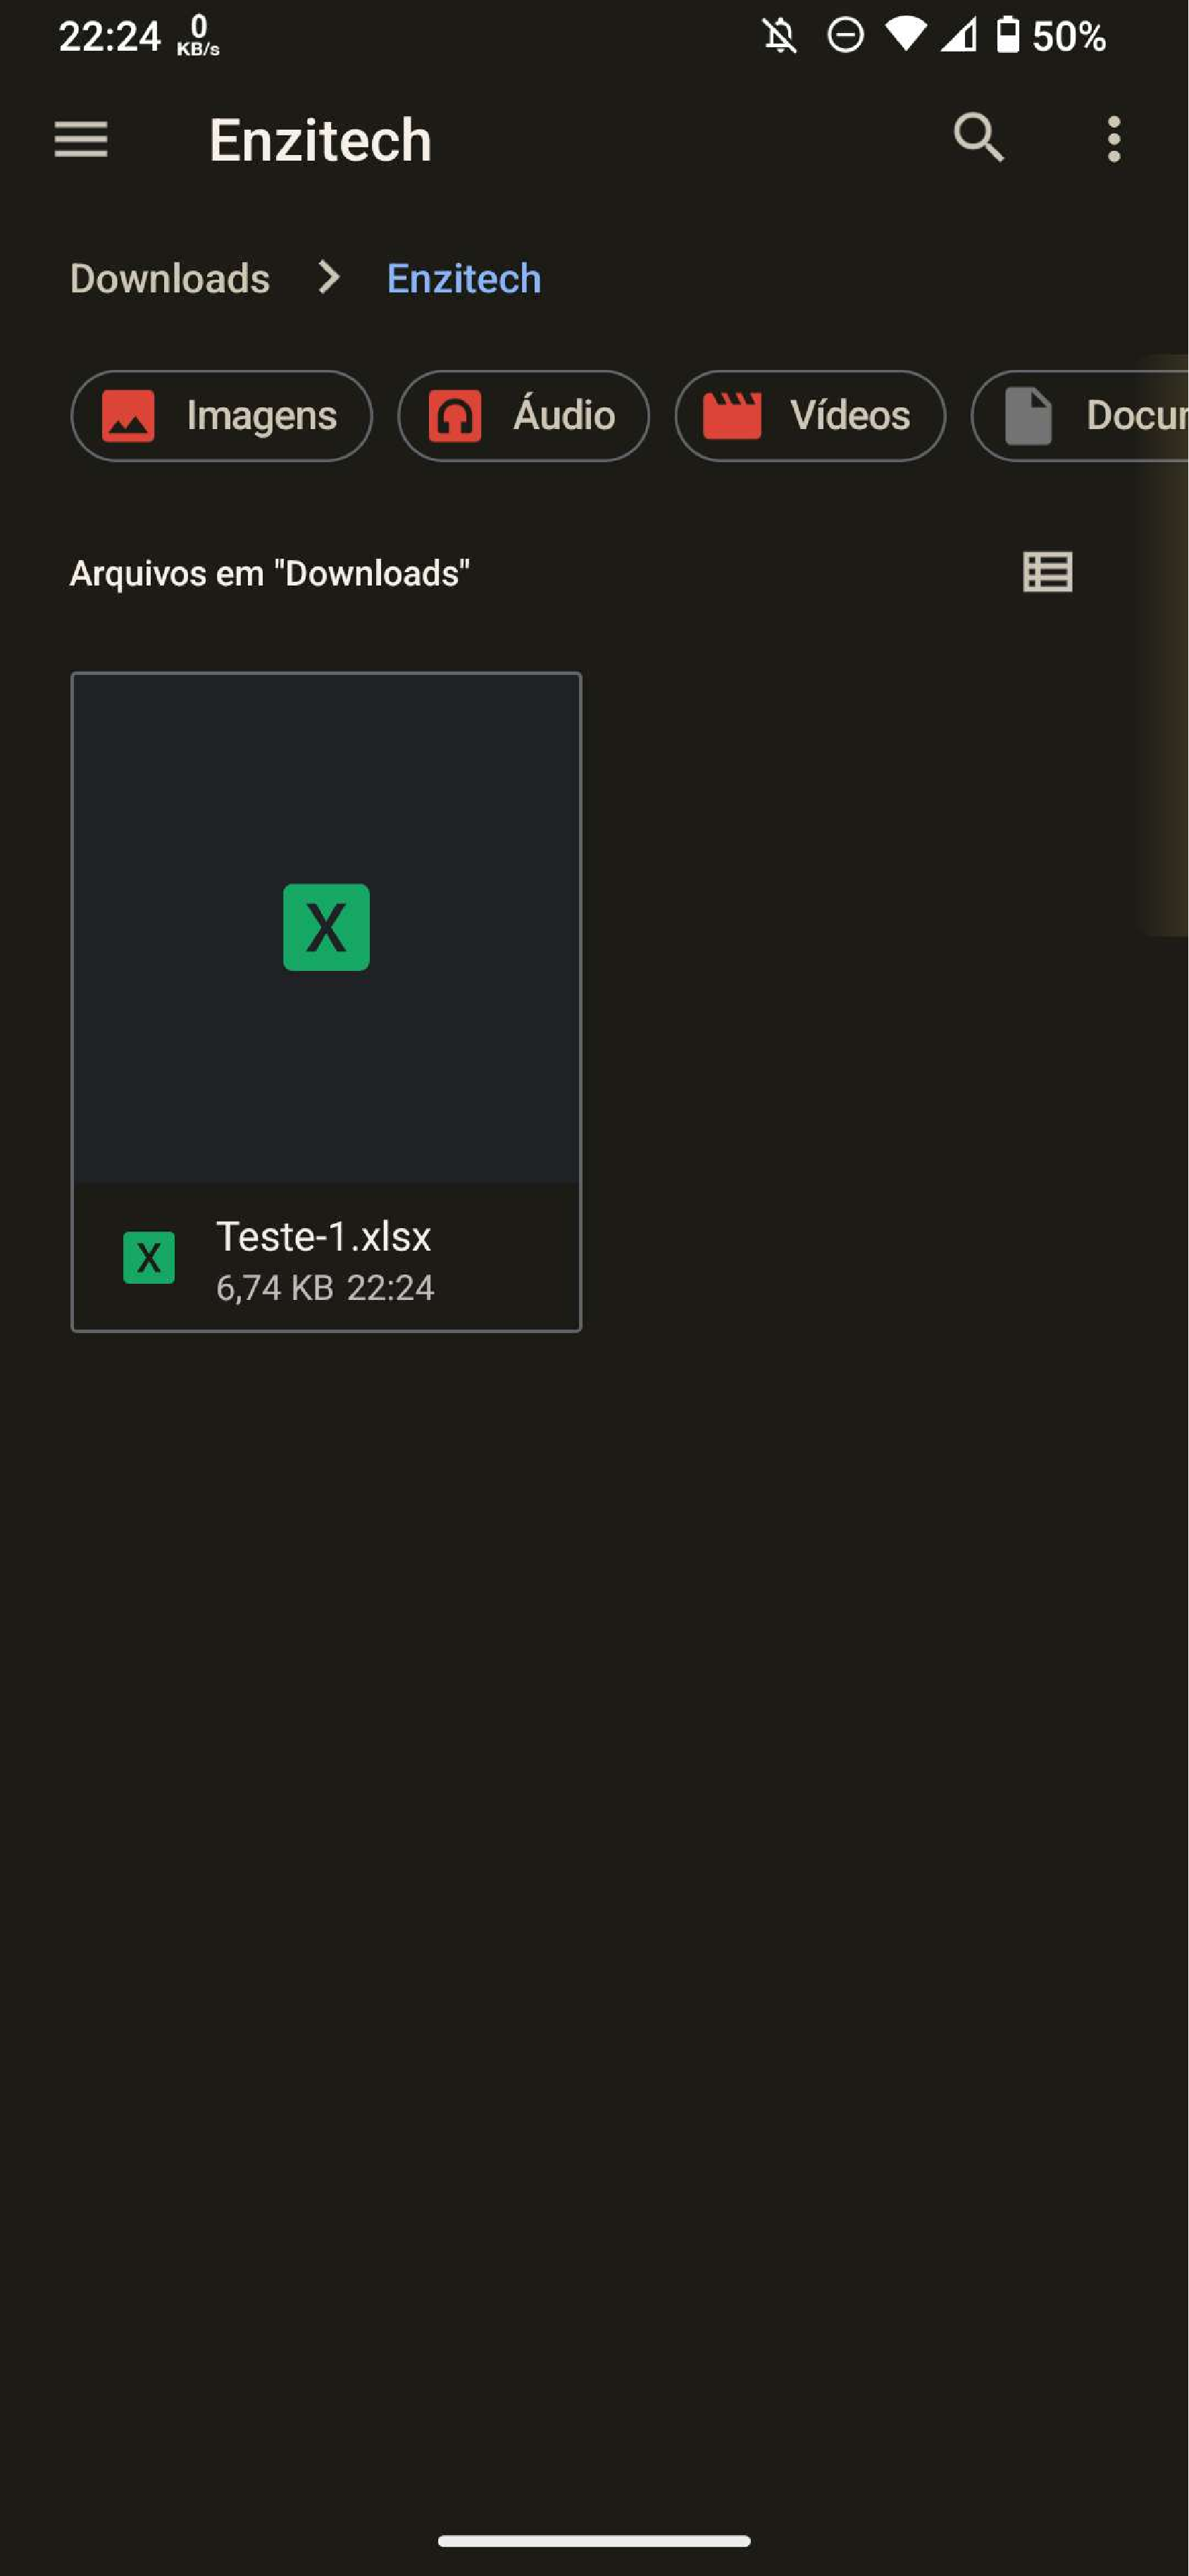
\includegraphics[width=.3\textwidth]{images/enzitech/resultados_salvar_downloads.pdf}
  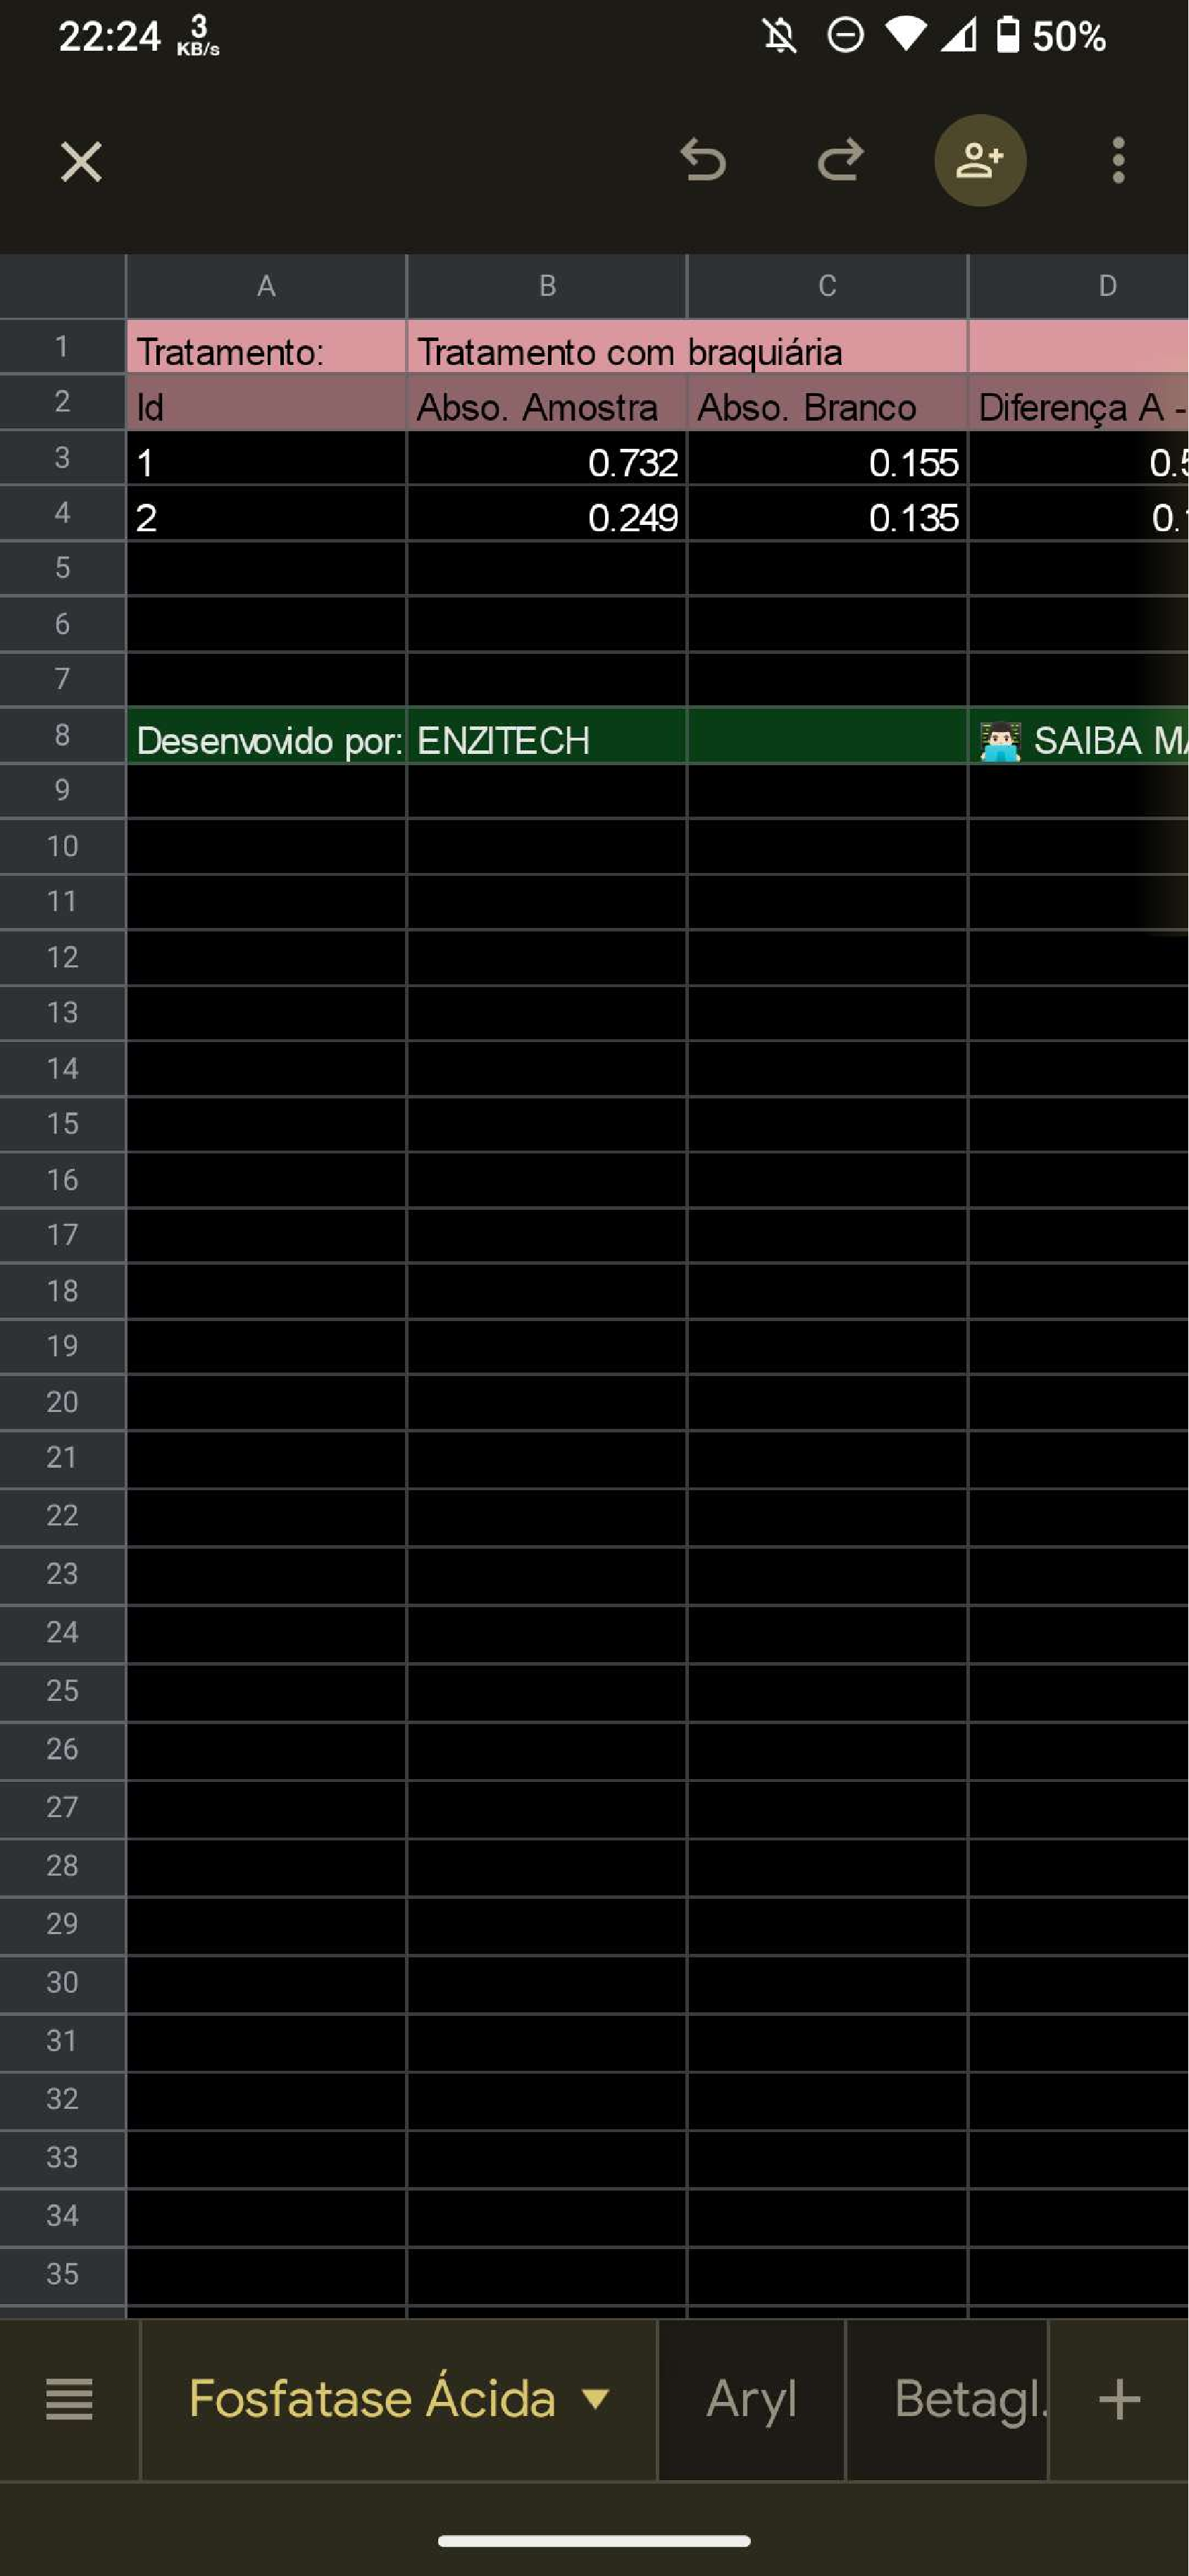
\includegraphics[width=.3\textwidth]{images/enzitech/resultados_salvar_planilha_min.pdf}
  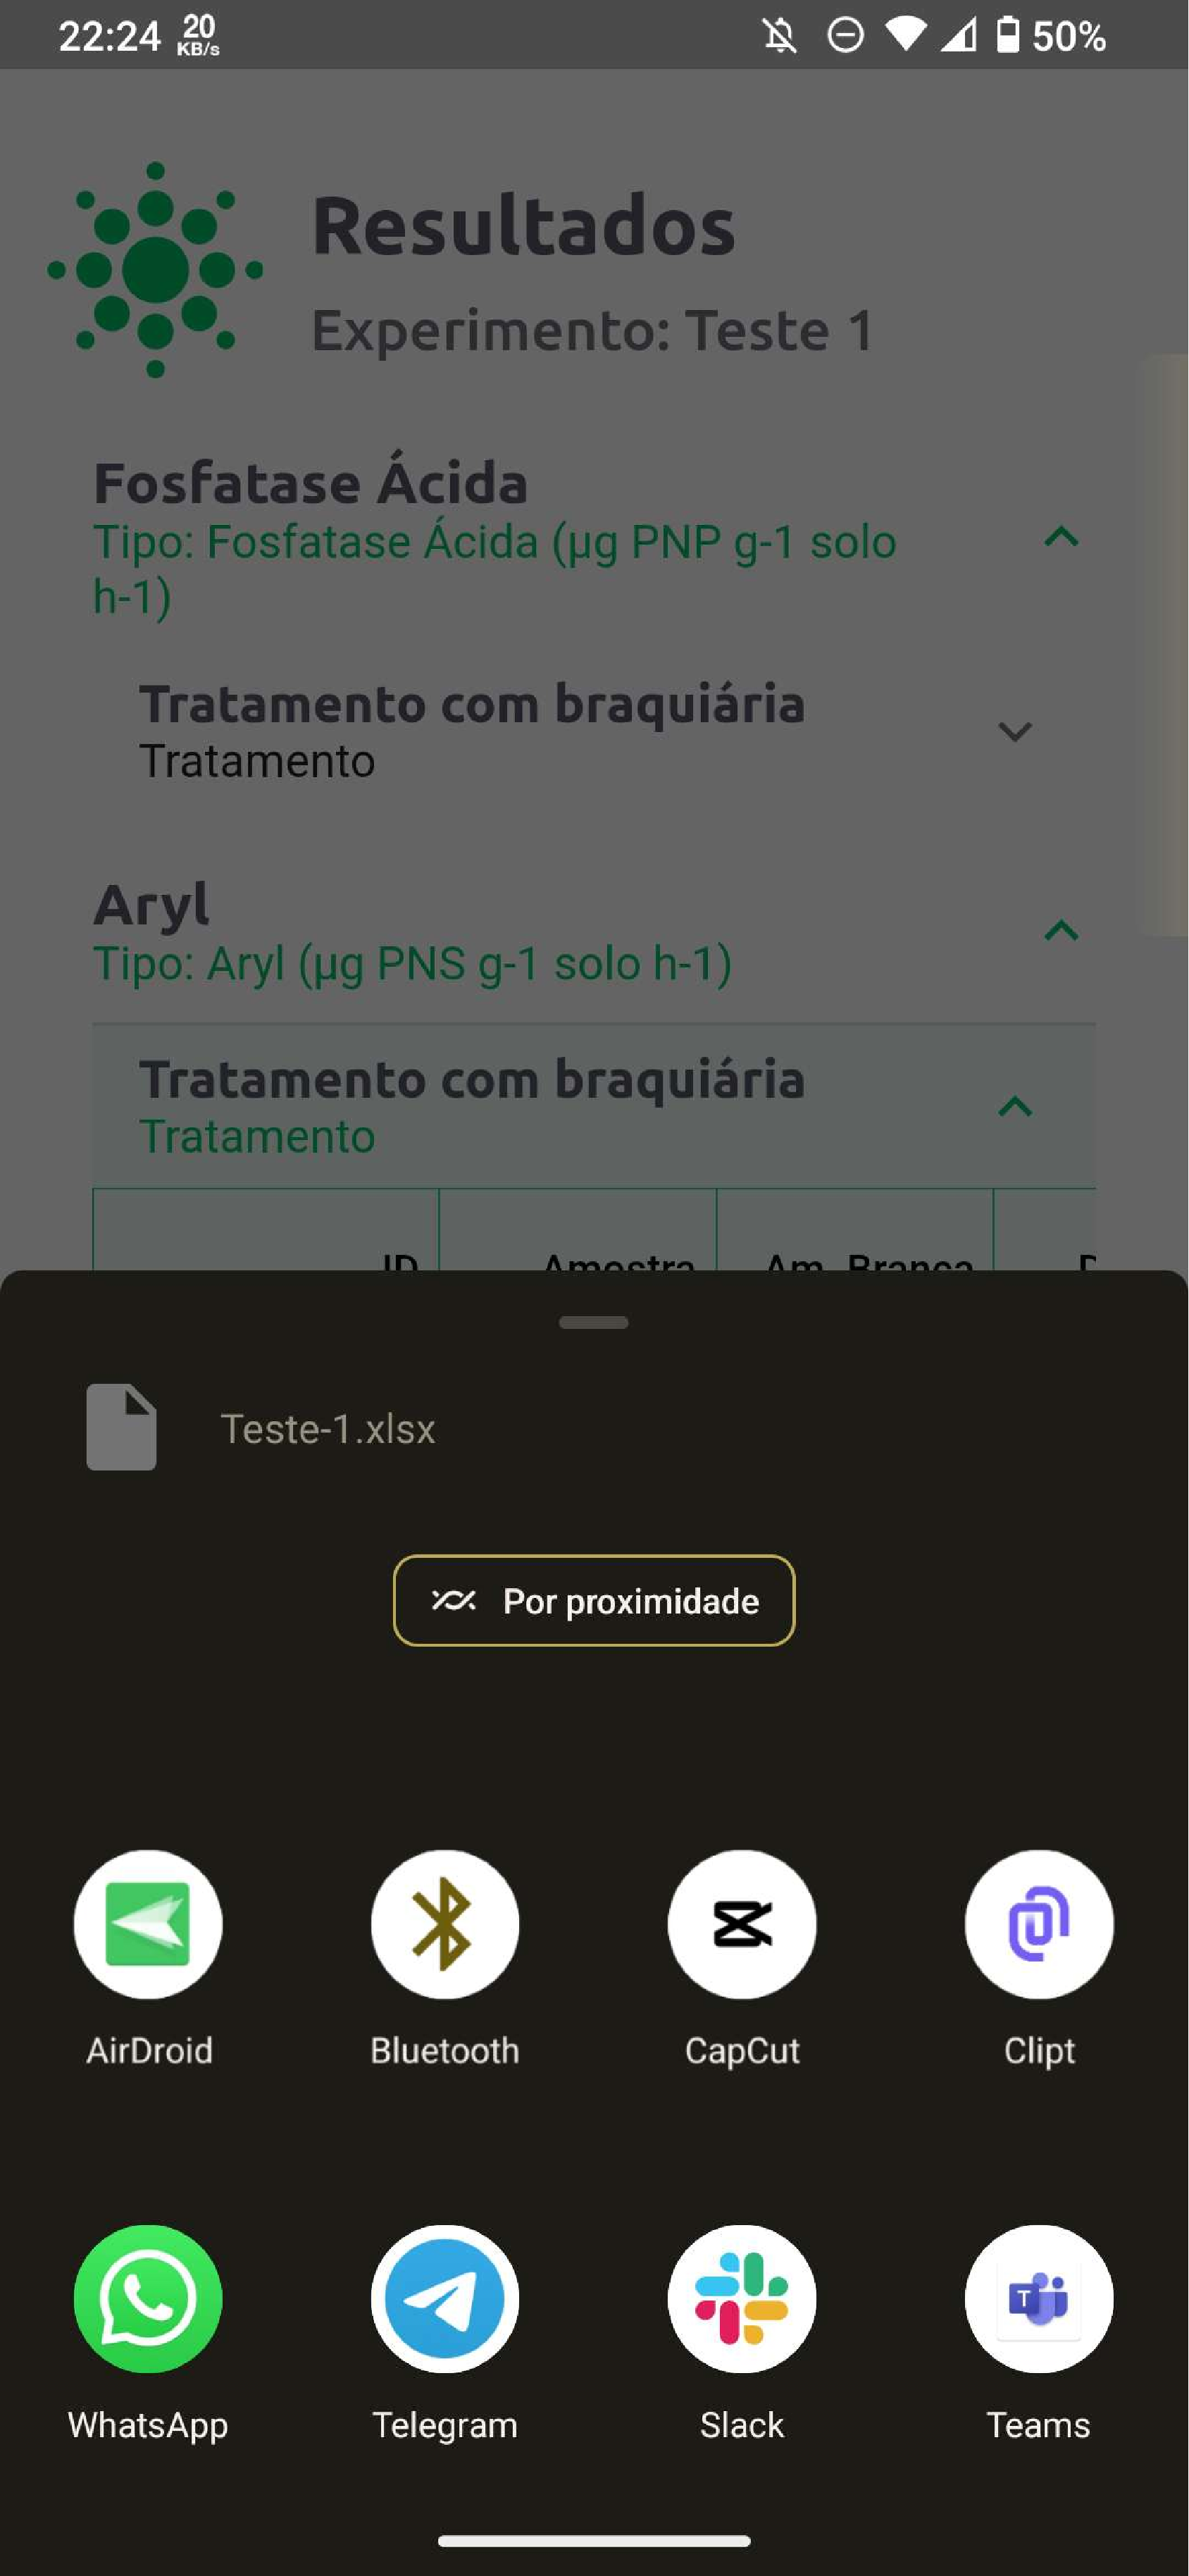
\includegraphics[width=.3\textwidth]{images/enzitech/compartilhar.pdf}

  \caption{Fluxo de visualização e compartilhamento de resultados de um experimento.}
  \label{fig:fluxo_resultados}
  \acsfont{Fonte: Aplicativo Enzitech desenvolvido pelo autor}
  
\end{figure}

As duas primeiras imagens do fluxo da \figref{fig:fluxo_resultados} são de experimentos diferentes, a primeira é de um que já foi concluído, nele é possível ver que o usuário tem a ação de cálculo enzimático bloqueado, já na segunda imagem é o experimento que seguirá o fluxo de visualização e compartilhamento dos resultados aqui, este experimento possui um tratamento, duas repetições, e cinco enzimas cadastradas.

Ao entrar nos resultados do experimento, o usuário consegue visualizar de forma organizada todos os dados preenchidos como uma listagem com tabelas para cada combinação de enzima e tratamento feita, nesta tela, é possível salvar o resultado em uma planilha Excel no formato \textsc{nome-do-experimento.xlsx} no armazenamento do dispositivo, como é possível ver na terceira, quarta e quinta imagem do fluxo da \figref{fig:fluxo_resultados}, a planilha é montada seguindo o mesmo padrão, para cada enzima é criado uma página, e dentro de cada página os resultados são montados com suas repetições para cada tratamento do experimento (caso de uso UC10).

Além disso, o usuário pode compartilhar diretamente o arquivo para qualquer \ac{app} externo que suporte esta ação, ao compartilhar um experimento, o salvamento dele também é realizado (caso de uso UC11).

Por fim, o usuário tem acesso à uma tela de configurações na \textit{home} do \ac{app} (\figref{fig:configuracoes_app}), nela é possível ter acesso às seguintes funcionalidades adicionais: informações do \ac{app}, seus dados de login, uma configuração para a ativação e desativação do \textit{AlertDialog} para confirmação da exclusão de itens no \ac{app}, informação da quantidade de resultados de experimentos salvos localmente, informações sobre ambiente e versão do \ac{app} e a opção de deslogar do sistema. Além, disso, como mostrado na última imagem, o \ac{app} tem uma funcionalidade que informa quando o aplicativo fica sem acesso ao servidor, seja por falha no servidor ou por problemas de conexão com a internet. Por fim, o \ac{app} também contempla a funcionalidade de armazenar e consumir dados em \textit{cache} quando não há conexão com a internet disponível, tornando possível a visualização de algumas informações resumidas.

\begin{figure}[H]
\centering
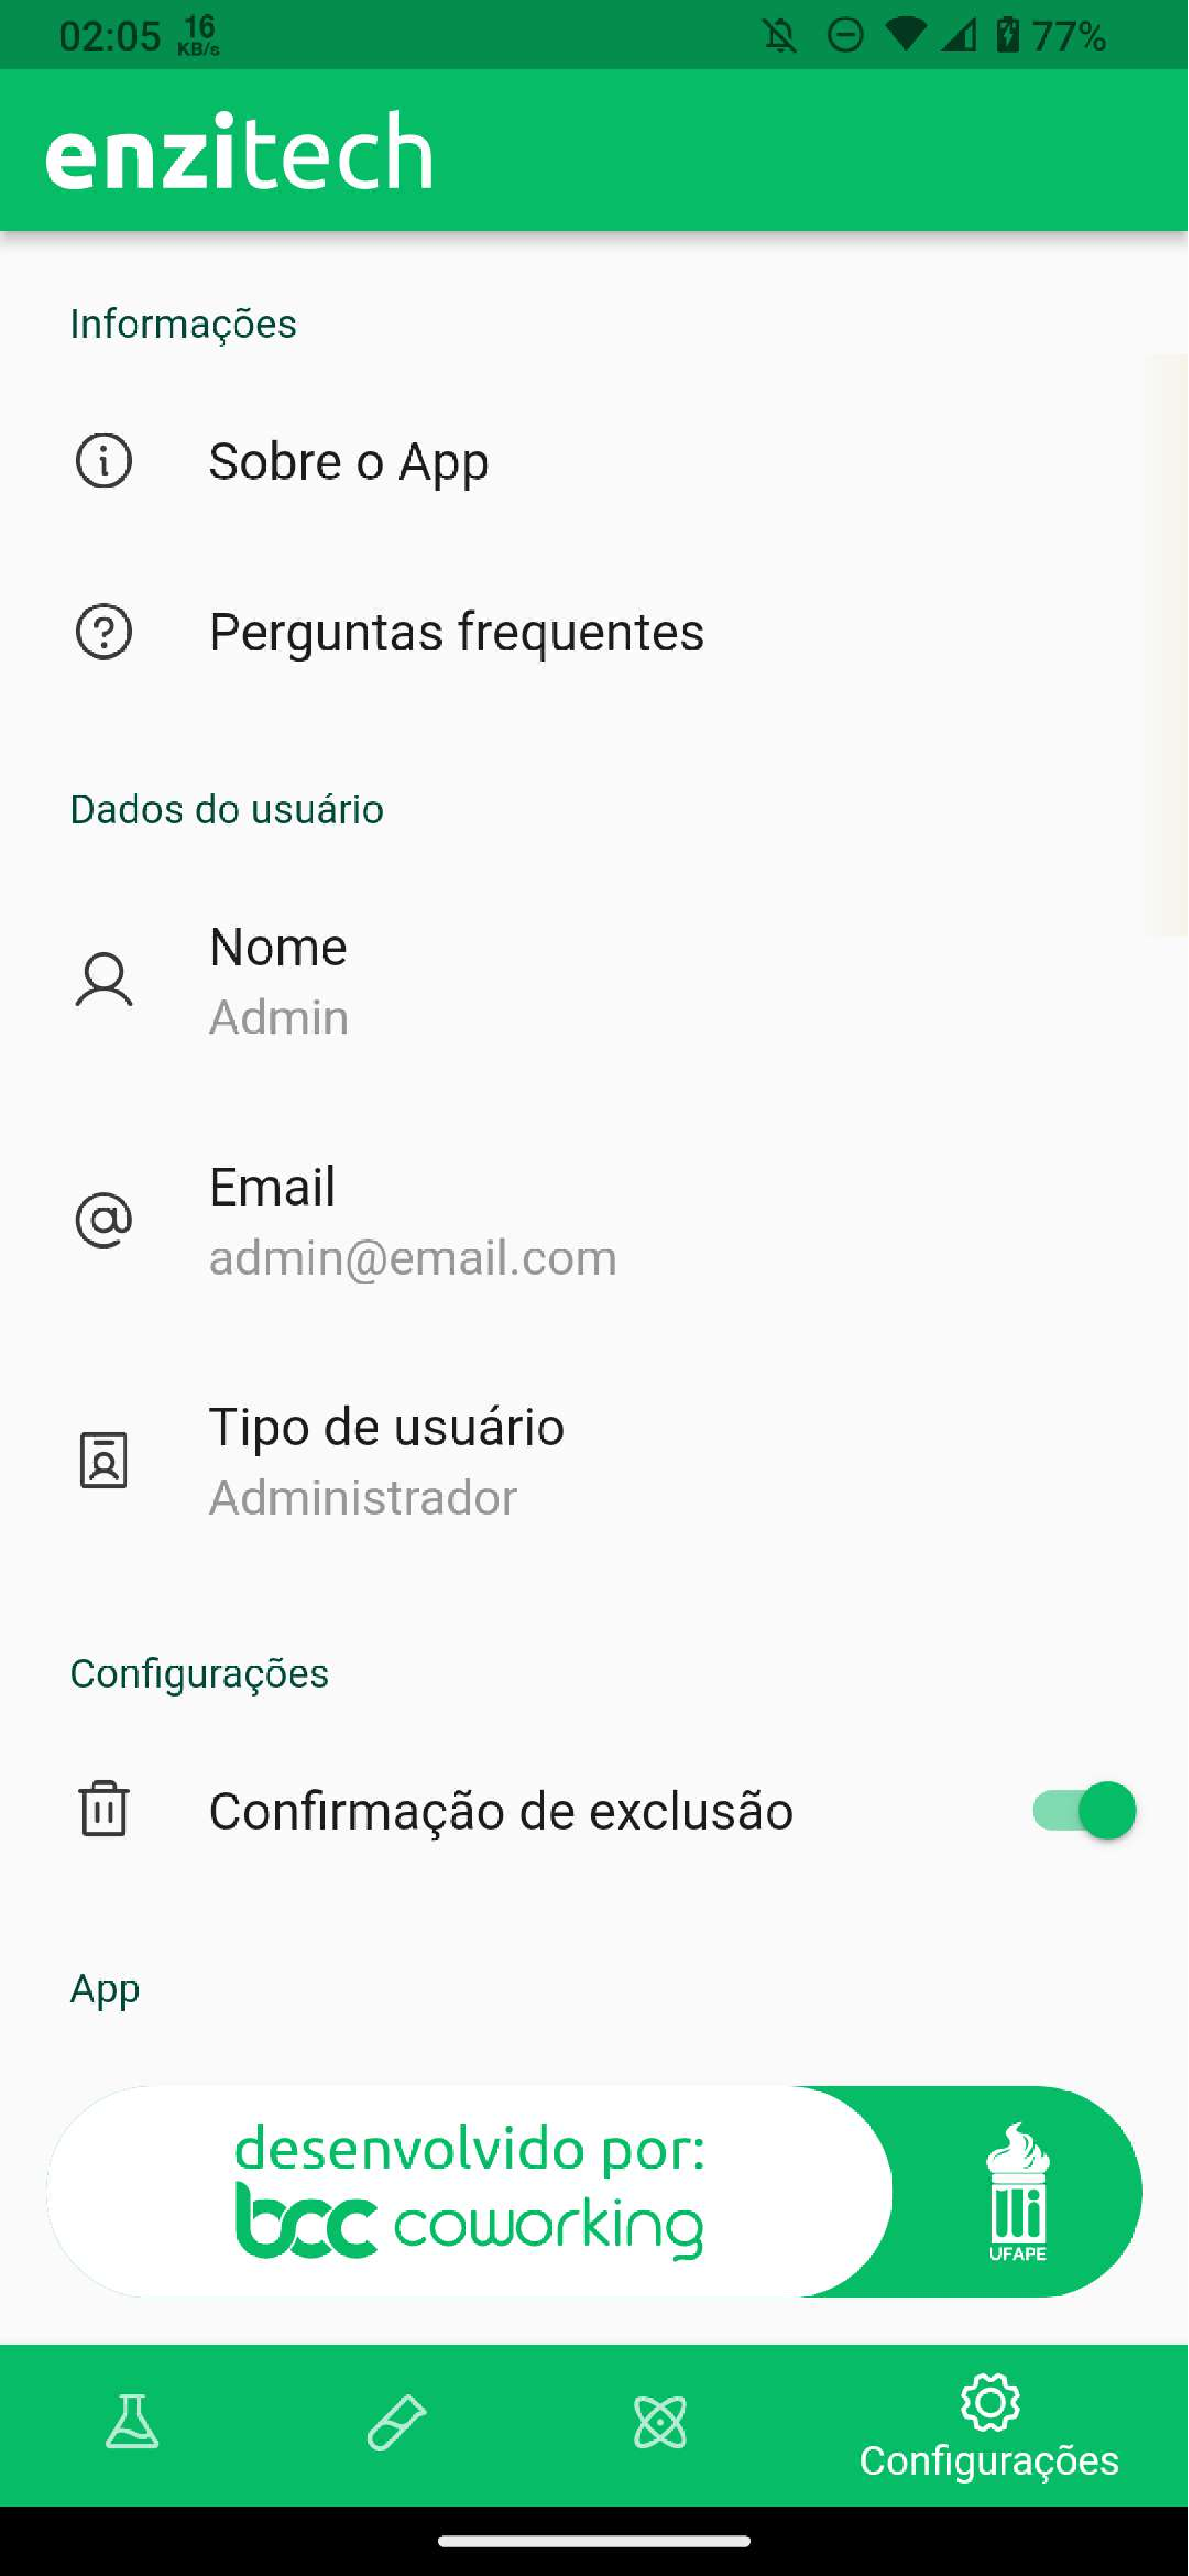
\includegraphics[width=.3\textwidth]{images/enzitech/config.pdf}\hfill
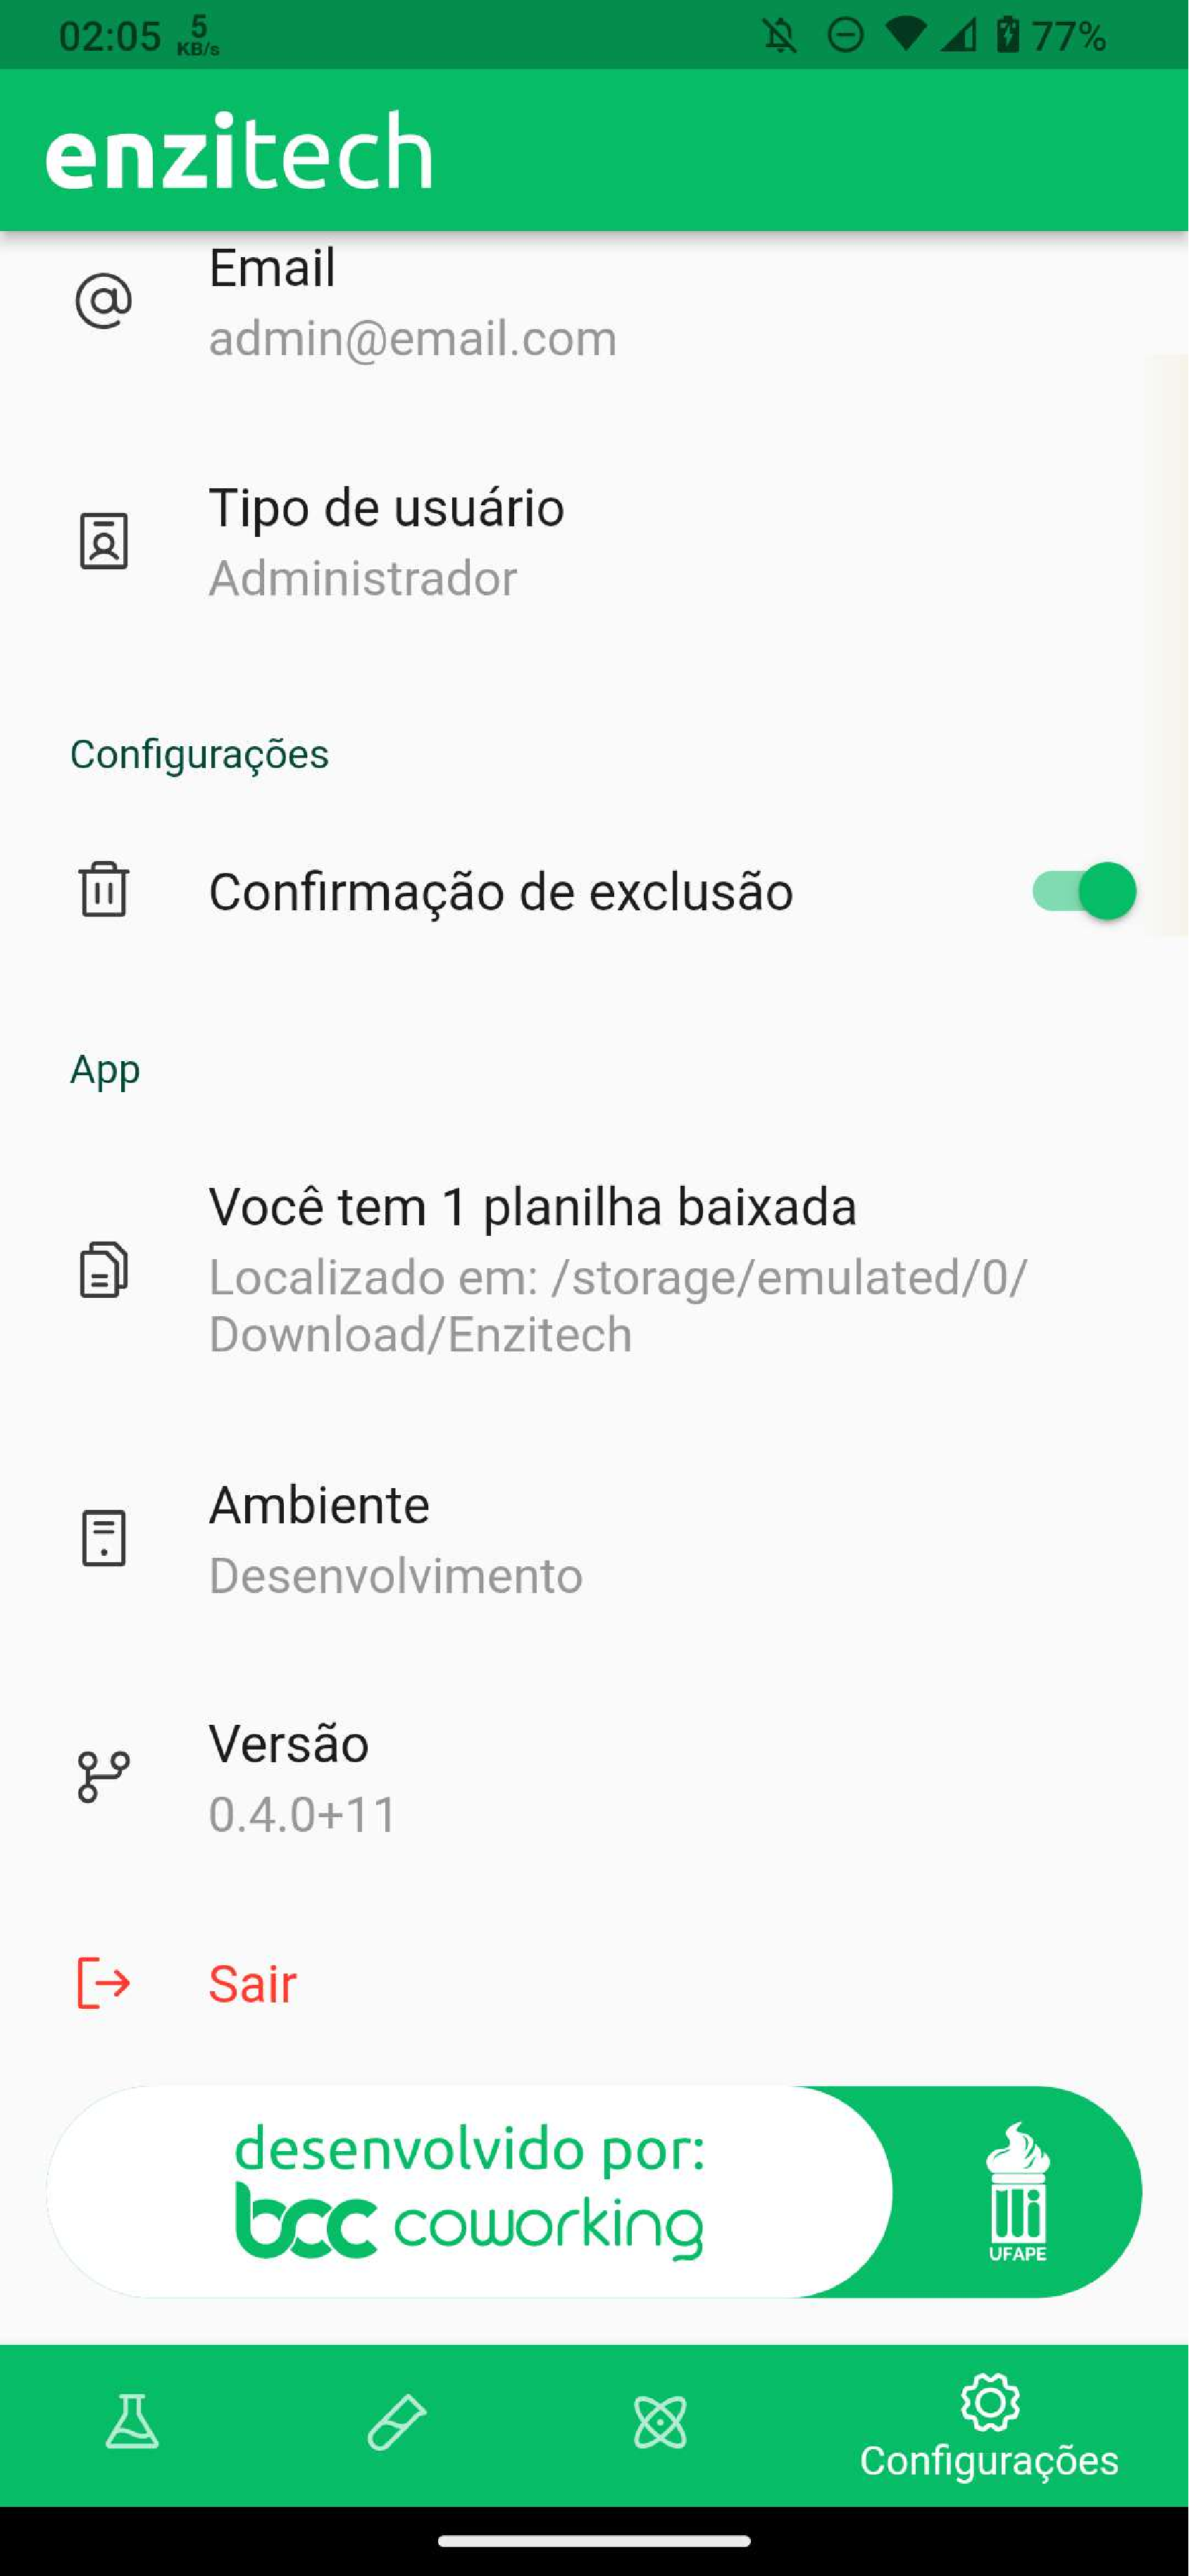
\includegraphics[width=.3\textwidth]{images/enzitech/config2.pdf}\hfill
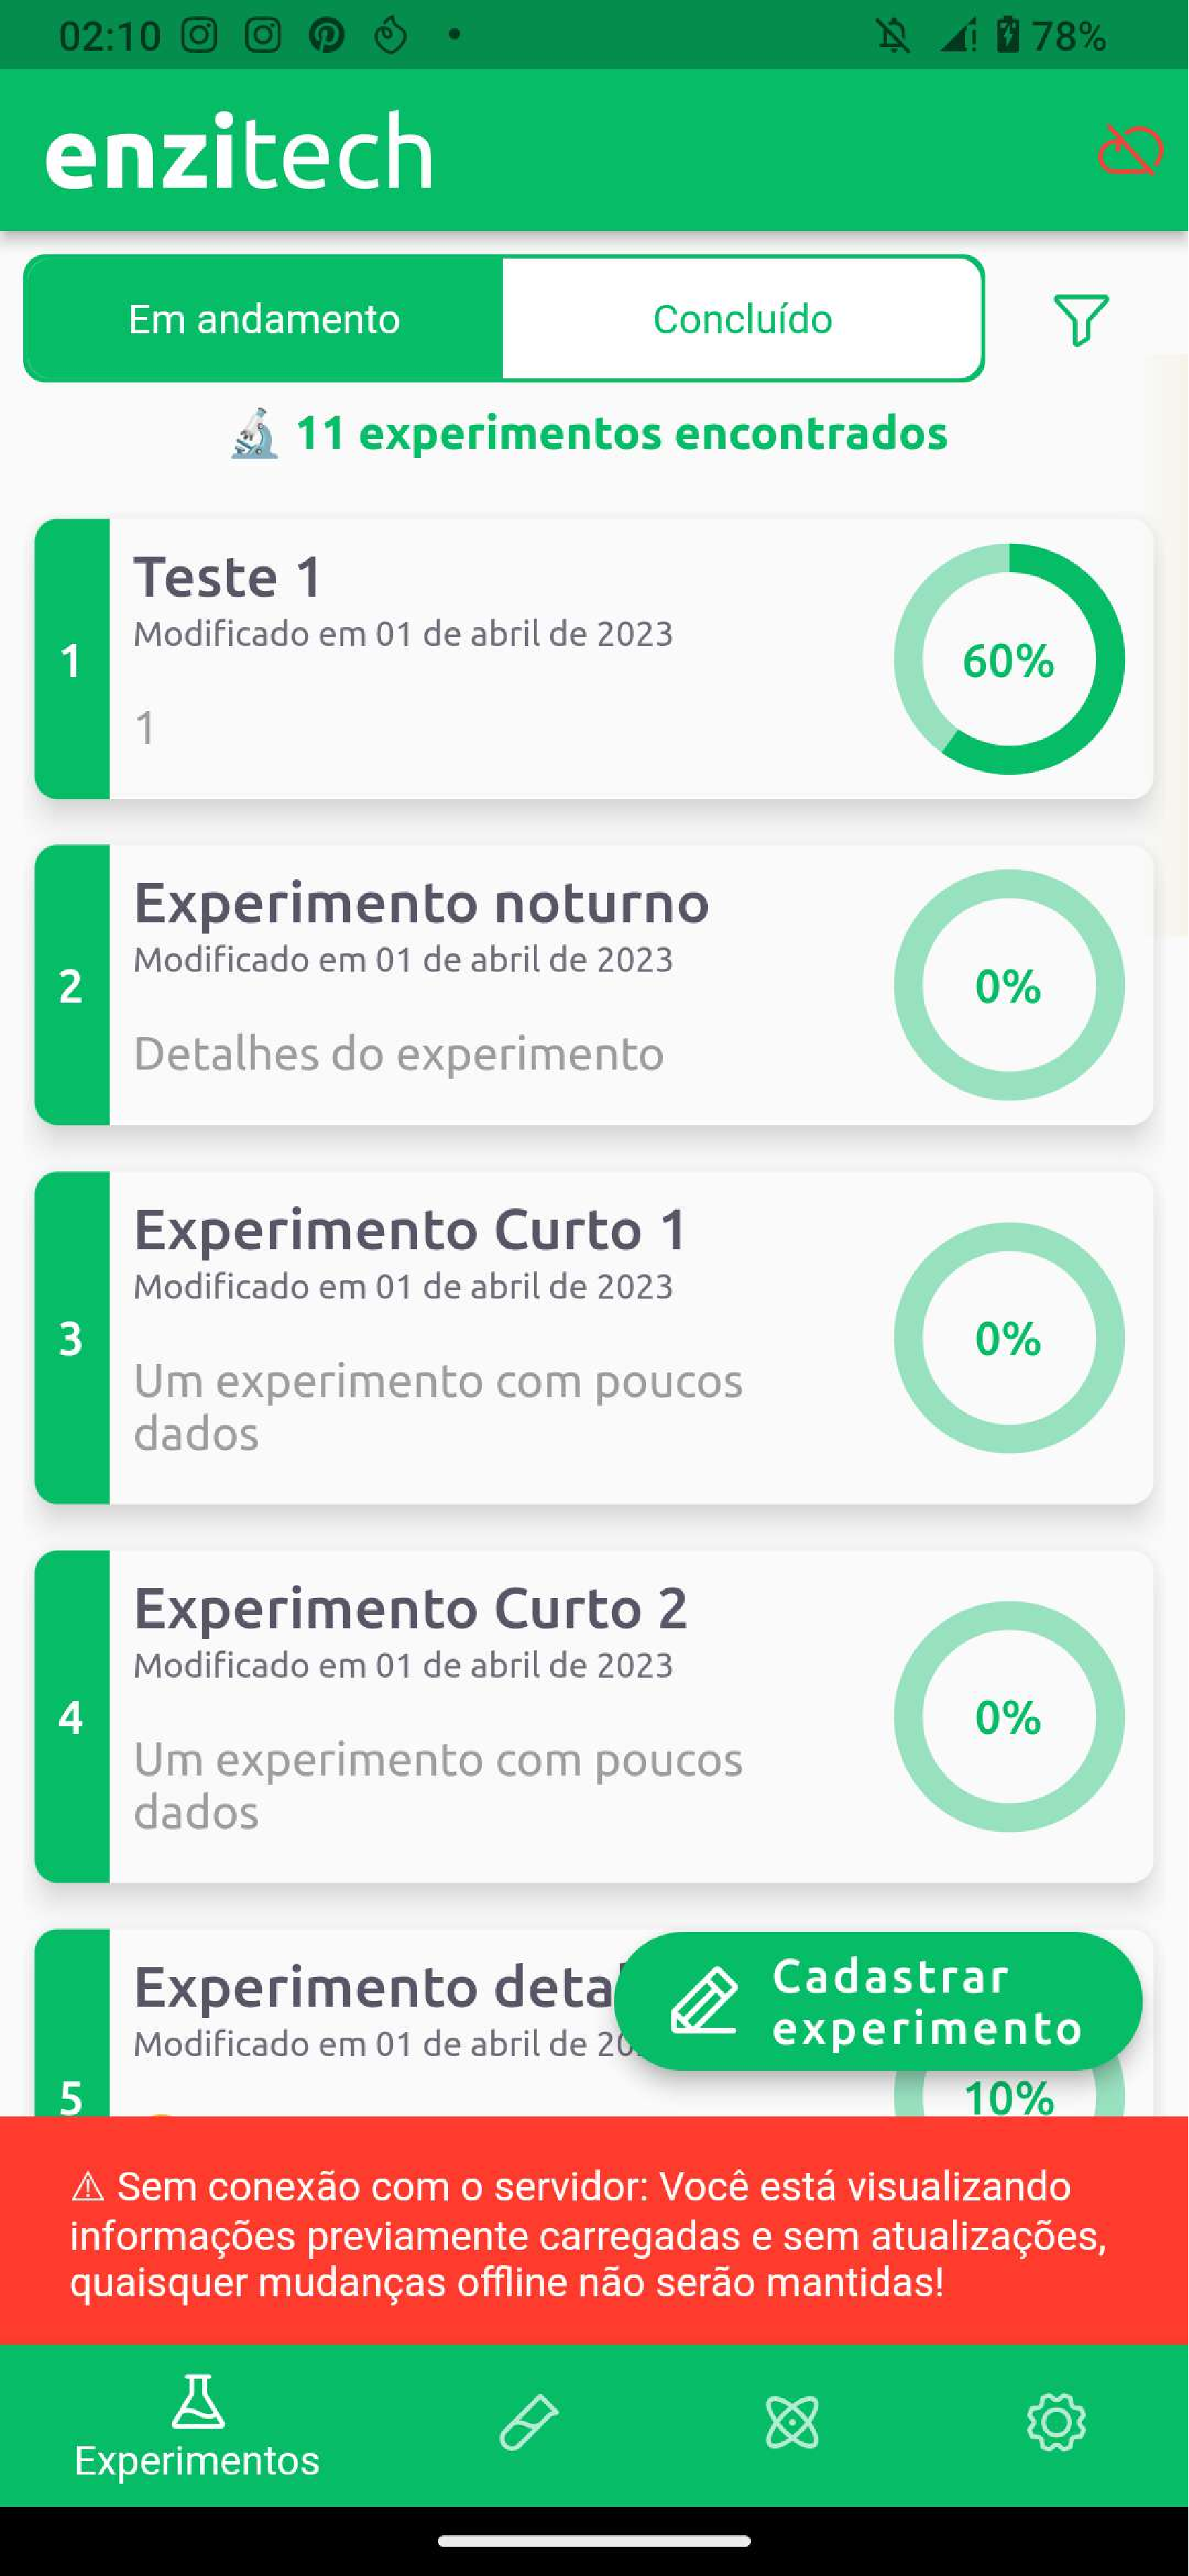
\includegraphics[width=.3\textwidth]{images/enzitech/offline.pdf}\hfill
\caption{Tela de configurações do \ac{app} do Enzitech.}
  \acsfont{Fonte: Aplicativo Enzitech desenvolvido pelo autor}
\label{fig:configuracoes_app}
\end{figure}

\chapter{Conclusão}

\section{Introduction}

\lipsum[1-4]

\section{Section}

\lipsum[2-4]

\subsection{Subsection}

\lipsum[2-4]

% References

\begin{references}
  \bibliography{references}
\end{references}

% Appendix

% \theappendix
% \chapter{Mapping Study's Instruments}
\label{ap:mapping-study}

\begin{table}[!htp]
	\centering
	\caption{List of conferences on which the searches were performed.}
	\label{tbl:conferences_list}
	\rowcolors{2}{lightgray!30}{white}
	\resizebox{\columnwidth}{!}{
	\begin{tabular}{ll}
	\toprule
	\textbf{Acronym} & \textbf{Conference} \\
	\toprule
	APSEC & Asia Pacific Software Engineering Conference \\
	ASE   & IEEE/ACM International Conference on Automated Software Engineering \\
	CSMR  & European Conference on Software Maintenance and Reengineering \\
	ESEC  & European Software Engineering Conference \\
	ESEM  & International Symposium on Empirical Software Management and Measurement \\
	ICSE  & International Conference on Software Engineering \\
	ICSM  & International Conference on Software Maintenance \\
	ICST & International Conference on Software Testing \\
	InfoVis & IEEE Information Visualization Conference \\
	KDD   & ACM SIGKDD International Conference on Knowledge Discovery and Data Mining \\
	MSR   & Working Conference on Mining Software Repositories \\
	OOPSLA & Object-Oriented Programming, Systems, Languages and Applications \\
	QSIC  & International Conference On Quality Software \\
	SAC & ACM Symposium on Applied Computing \\
	SEAA & EUROMICRO Conference on Software Engineering and Advanced Applications\\
	SEDE & 19th International Conference on Software Engineering and Data Engineering \\
	SEKE  & International Conference on Software Engineering and Knowledge Engineering \\
	\bottomrule
	\end{tabular}
	}
\end{table}

\begin{table}[htp]
	\caption{List of journals in which the searches were performed.}
	\label{tbl:journals_list}
	\centering
	\rowcolors{2}{lightgray!30}{white}
	\begin{tabular}{l}
	\toprule
	\textbf{Journal title} \\
	\toprule
	ACM Transactions on Software Engineering and Methodology \\
	Automated Software Engineering \\
	Elsevier Information and Software Technology \\
	Elsevier Journal of Systems and Software \\
	Empirical Software Engineering \\
	IEEE Software \\
	IEEE Computer \\
	IEEE Transactions on Software Engineering \\
	International Journal of Software Engineering and Knowledge Engineering \\
	Journal of Software: Evolution and Process \\
	Software Quality Journal \\
	Journal of Software \\
	Software Practice and Experience Journal \\
	\bottomrule
	\end{tabular}
\end{table}

\begin{table}[h]
\centering
\footnotesize
 \rowcolors{2}{lightgray!30}{white}
\caption{Search string per Search Engine.}
\label{tbl:stringengine}
\begin{tabular}{p{.15\textwidth}p{.8\textwidth}}
\toprule
\textbf{Search Engine} & \textbf{Search String}\\
\toprule
   	 	Google Scholar &  bug report OR track OR triage ``change
   	 	request'' issue track OR request OR software OR ``modification request'' OR
   	 	``defect track'' OR ``software issue''  repositories maintenance evolution\\

   	 	ACM Portal & Abstract: "bug report" or Abstract:"change request"
   	 	or Abstract:"bug track" or Abstract:"issue track" or  Abstract:"defect
   	 	track" or Abstract:"bug triage" or Abstract: "software issue" or Abstract: "issue request"
   	 	or Abstract: "modification request") and  (Abstract:software or
   	 	Abstract:maintenance or Abstract:repositories or Abstract:repository \\

   	 	IEEExplorer (1) & (((((((((("Abstract": "bug report") OR
   	 	"Abstract":"change request") OR "Abstract":"bug track") OR "Abstract":"software issue") OR "Abstract":"issue request") OR
        "Abstract":"modification request") OR "Abstract":"issue track") OR
	    "Abstract":"defect track") OR "Abstract":"bug triage") AND
	    "Abstract":software)\\

         IEEExplorer (2) & (((((((((("Abstract": "bug report") OR
         "Abstract":"change request") OR "Abstract":"bug track") OR "Abstract":"software issue") OR
         "Abstract":"issue request") OR "Abstract":"modification request") OR
         "Abstract":"issue track") OR "Abstract":"defect track") OR
         "Abstract":"bug triage") AND "Abstract":maintenance)\\

         IEEExplorer (3) & (((((((((("Abstract": "bug report") OR
         "Abstract":"change request") OR "Abstract":"bug track") OR "Abstract":"software issue") OR
         "Abstract":"issue request") OR "Abstract":"modification request") OR
         "Abstract":"issue track") OR "Abstract":"defect track") OR
         "Abstract":"bug triage") AND "Abstract":repositories)\\

         IEEExplorer & (((((((((("Abstract": "bug report") OR
         "Abstract":"change request") OR "Abstract":"bug track") OR "Abstract":"software issue") OR
         "Abstract":"issue request") OR "Abstract":"modification request") OR
         "Abstract":"issue track") OR "Abstract":"defect track") OR
         "Abstract":"bug triage") AND "Abstract": repository)\\

         Citeseer Library & (abstract: "bug report" OR abstract:"change request" OR abstract:"bug track" OR abstract:"issue track" OR
	     abstract:"defect track" OR abstract:"bug triage" OR abstract: "software
	     issue" OR abstract: "issue request" OR abstract: "modification request")
	     AND (abstract:software OR abstract:maintenance OR abstract:repositories OR
	     abstract:repository)\\

	     Elsevier & ("bug report" OR "change
	     request" OR "bug track" OR "issue track" OR "defect track" OR "bug triage" OR "software issue" OR  "issue request" OR
	    "modification request") AND (software OR maintenance OR repositories OR
	    repository)\\

	    Scirus & ("bug report" OR "change request" OR "bug track" OR "issue track" OR  "defect track" OR "bug triage" OR
        "software issue" OR  "issue request" OR "modification request") AND
	    (software maintenance OR repositories OR repository) ANDNOT (medical OR
	    aerospace)\\

	    ScienceDirect & ("bug report" OR "change request" OR "bug track"
	     OR "issue track" OR "defect track" OR "bug triage" OR "issue request" OR
	     "modification request") AND LIMIT-TO(topics, "soft ware")\\

	     Scopus & ("bug report" OR "change request" OR "bug track" OR
	     "issue track" OR  "defect track" OR "bug triage" OR "software issue" OR
	     "issue request" OR "modification request") AND (software maintenance OR
	     repositories OR repository)\\

	     Wiley & ("bug report" OR "change request"
	     OR "bug track" OR "issue track" OR  "defect track" OR "bug triage" OR
         "software issue" OR  "issue request" OR "modification request") AND
	     (software maintenance OR repositories OR repository)\\

	     ISI Web\newline of Knowledge & ("bug report" OR "change request" OR "bug
	     track" OR "issue track" OR  "defect track" OR "bug triage" OR "software issue" OR  "issue request" OR "modification request") AND
	    (software maintenance OR repositories OR repository) ANDNOT (medical OR
	    aerospace)\\

	    SpringerLink & ("bug report" OR "change request" OR "bug track" OR "issue track" OR  "defect track" OR "bug triage" OR
        "software issue" OR  "issue request" OR "modification request") AND
	    (software maintenance OR repositories OR repository) ANDNOT (medical OR
	    aerospace)\\
	\bottomrule
\end{tabular}
\end{table}

\end{document}
